\documentclass[10pt,a4paper]{book}



%\usepackage{a4wide}
\usepackage[left=2.50cm, right=2.50cm, top=2.50cm, bottom=2.50cm]{geometry}
\usepackage{bm}
\usepackage{natbib
}\usepackage{amsmath}
\usepackage{amssymb}
\usepackage{graphicx}
%\usepackage{pslatex}
%\usepackage{palatino}
%\usepackage{bookman}
%\usepackage{times}
%\usepackage{mathptmx}
%\usepackage{mathpazo}

%\usepackage{ascii}
%\usepackage{hyperref}

\usepackage{caption}
\usepackage{subcaption}

\usepackage{varioref}


\newcommand{\He}{\mathcal{H}}
\newcommand{\G}{\mathcal{G}}
\newcommand{\p}{\partial}
\newcommand{\eps}{\dot{\epsilon}}
\newcommand{\de}{\delta}
\newcommand{\eij}{\dot{\epsilon}_{ij}}
\newcommand{\epq}{\dot{\epsilon}_{pq}}
\newcommand{\eii}{\dot{\epsilon}_{ii}}
\newcommand{\exx}{\dot{\epsilon}_{xx}}
\newcommand{\eyy}{\dot{\epsilon}_{yy}}
\newcommand{\ezz}{\dot{\epsilon}_{zz}}
\newcommand{\exz}{\dot{\epsilon}_{xz}}
\newcommand{\eyz}{\dot{\epsilon}_{yz}}
\newcommand{\exy}{\dot{\epsilon}_{xy}}
\newcommand{\sij}{\sigma_{ij}}
\newcommand{\tij}{\tau_{ij}}
\newcommand{\tbx}{t_{bx}}
\newcommand{\tby}{t_{by}}
\newcommand{\txx}{\tau_{xx}}
\newcommand{\tyy}{\tau_{yy}}
\newcommand{\tzz}{\tau_{zz}}
\newcommand{\txy}{\tau_{xy}}
\newcommand{\txz}{\tau_{xz}}
\newcommand{\tyz}{\tau_{yz}}
\newcommand{\sxx}{\sigma_{xx}}
\newcommand{\sxy}{\sigma_{xy}}
\newcommand{\sxz}{\sigma_{xz}}
\newcommand{\syy}{\sigma_{yy}}
\newcommand{\syz}{\sigma_{yz}}
\newcommand{\szz}{\sigma_{zz}}
\newcommand{\normal}{\hat{\bm{n}}}
\newcommand{\normalh}{\hat{\bm{n}}_h}
\newcommand{\I}{\mathrm{i}}
\newcommand{\Ua}{\textsl{\'Ua}\,}
\newcommand{\xgl}{x_{\mathrm{gl}}}

\providecommand{\abs}[1]{\lvert#1\rvert}
\providecommand{\norm}[1]{\lVert#1\rVert}


\title{\Ua\\{\it Compendium}}
\author{G.~Hilmar Gudmundsson\\ \\ \textit{University of Northumbria}}

\begin{document}

\maketitle
\tableofcontents

\frontmatter



\chapter{Introduction}
\Ua is a finite-element ice flow model.  This document provides some
theoretical background information to \Ua. It is not a manual. This is
a `life' document, i.e.\ it is constantly being modified and changed
and the current from of the document is in no means final. It contains
some general material on glacier mechanics, a bit on the FE method,
and lots of some very specific \Ua related stuff.  Most of the
material related stricly to glacier mechanics is from a course given
at Caltech in 2014.

\chapter{Notation and definitions}



\begin{figure}
\centerline{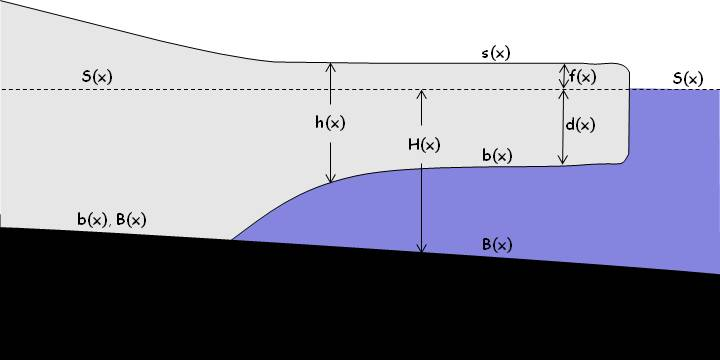
\includegraphics[width=12cm]{ProblemGeometry.jpg}}
\caption{Geometrical variables: Glacier surface ($s$)), glacier bed ($b$), ocean surface ($S$), ocean floor ($B$), 
glacier thickness ($h=s-b$)), ocean depth ($H=S-B$), glacier draft ($d=S-b$), glacier freeboard ($f=s-S$). 
\label{fig:PG}}
\end{figure}

\begin{table}
\caption{\label{tab:geo1} List of variables}
\begin{center}
\begin{tabular}{cl}
\hline
$s$ & upper glacier surface \\
$b$ & lower glacier surface \\
$S$ & ocean surface \\
$B$ & bedrock / ocean floor \\
$h:=s-b$ & glacier thickness \\
$H:=S-B$ & ocean depth (pos.\ or neg.\ depending on location) \\
$H_{+} = \He(H) H$ & (positive) ocean depth \\
$d:=\He(H) (S-b$) & glacier draft (positive by definition) \\
$f:=s-S$ & freeboard (always positive) \\
$ \G:=\He(h-h_f)$ & grounding mask, 1 if ice grounded, 0 otherwise. \\
$h_f:=\rho_o H /\rho$ & maximal ice thickness without grounding \\
$\alpha$                    & tilt of coordinate system\\
$\rho$ & ice density \\
$\rho_o$ & ocean density \\
$\varrho =\rho \, (1-\rho/\rho_o)$ & \\
$(u_b,v_b,w_b) $ & $xyz$ components of basal velocity \\
$(u_s,v_s,w_s) $ & $xyz$ components of surface velocity \\
$\txx$, $\tyy$, $\txy$ etc. & deviatoric stress components \\
$\sxx$, $\syy$, $\sxy$ etc. & Cauchy stress components\\
$\exx$, $\eyy$, $\exy$ etc. & strain rates \\
$g$                         & gravitational acceleration\\

\hline
\end{tabular}
\end{center}
\end{table}


Typical problem geometry is depicted in Fig.~\ref{fig:PG} and the main
geometrical variables listed in Table~\ref{tab:geo1}.  Upper and lower
glacier surfaces are denoted by $s$ and $b$, respectively, while the
ocean surface and the bedrock are denoted by $S$ and $B$,
respectively.  The ice thickness is $h=s-b$ and is always
positive. The distance from bedrock ($B$)) to the ocean surface ($S$)
is $H=S-B$, and this quantity can be either positive or negative,
depending on location.

The maximal ice thickness possible without grounding is denoted by $h_f$ and is
\[
h_f :=(S-B) \rho_o/\rho ,
\]
where $\rho$ and $\rho_o$ are  the ice and the ocean densities, respectively. 


The freeboard is
\[
f:=s-S,
\]
and the draft $d$ is defined as
\[
d:=\begin{cases} S-b , & \mbox{if } \, S>b \\  0 , & \hbox{otherwise }  \end{cases}
\]
which can also be written as
\[
d=\He(H) (S-b) ,
\]
where $\He(x)$ is the Heaviside function, defined as

\[ \He(x)=  \begin{cases} 
              0 & \text{for}   \quad x < 0 \\          
             1/2 & \text{for}  \quad x=1/2 \\
             1 & \text{for}    \quad x>0
   \end{cases}
\]

The function $\He(h-h_f)$ (equal to one if grounded, zero if afloat), is needed frequently and we define $\G$ as
\[
\G=\He(h-h_f)
\]
Hence
\begin{equation} \G =  \He(h-h_f) = \begin{cases} 
              0 & \text{over floating areas}    \\          
             1/2 & \text{at the grounding line}\\
             1 & \text{over grounded areas}   \\
   \end{cases}
\label{eq:Gdef}
\end{equation}
The variable $\G$ can the thought of as a `grounding' parameter.

The `positive' ocean depth $H_{+}$ is defined as
\begin{equation}
H_{+} := \He(H) H ,
\label{eq:Hplus}
\end{equation}
i.e.\ $H_{+}=H$ if $H>0$ and zero otherwise.




To distinguish between continuous quantities and discrete quantities we
use bold face for the latter.  In a finite-element context we might
write
\[ 
f(x) = f_q \, \phi_q(x) 
\]
Here $f$ is a continuous function, $f_q$ the nodal variables, and
$\phi_q$ the shape/form functions. We sometimes group the nodal
variables together into a vector writing
\[
\bm{f}=[f_1, f_1, \dots , f_N]^T
\]
and then
\[
f(x) = \bm{f}^T \bm{\phi}
\]
Note that $f$ and $f_q$ very are different quantities. If, for a vector
$\bm{f}$, we need to refer to the $q$ element of the vector, we write
$[\bm{f}]_q$, i.e.
\[
f_q=[\bm{f}]_q
\] 
The matrix representation of a continuous operator $L: H_1 \to H_2$ is
written in bold as $\bm{L}$. The elements of the matrix are
$L_{pq}=[\bm{L}]_{pq}$.

The $L^2$ norm is 
\[
 (f,g)_{L^2} = \int f(x) \, g(x) \, dx
 \]
 where $f$ and $g$ are square intergrable functions and the $l^2$ norm
 is
\[
(\bm{f}, \bm{g} )_{l^2} = \bm{f}^T \cdot \bm{g}
\]
where $\bm{f}$ and $\bm{g}$ are vectors. The inner products define
corresponding $L^2$ and $l^2$ norms.

We often need to linearise various quantities, which we do by
calculating directional derivatives. The directional derivative $D \bm{f}$ of a
function $\bm{f}$ of the variable $\bm{x}$ in the direction $\bm{v}$ is defined as
\[
  D \bm{f}[\bm{x} ; \bm{v}] = \lim_{\epsilon \to 0} \frac{d}{d \epsilon} \bm{f}(\bm{x}+\epsilon \bm{v})
\]
Often we think of $\bm{v}$ being a small perturbation to $\bm{x}$ in which case we write
\[
  D \bm{f}[\bm{x} ; \Delta \bm{x}] = \lim_{\epsilon \to 0} \frac{d}{d \epsilon} \bm{f}(\bm{x}+\epsilon \Delta \bm{x})
\]
and may then simply write $D \bm{f}[\bm{x}]$.  Another common notation for the
directional derivative of the function $\bm{f}(\bm{x})$ in the
direction $\bm{v}$ is $\nabla_{\bm{v}} \bm{f}(\bm{x})$.
  






\mainmatter
\part{\Ua Stuff}
\chapter{Equations of ice flow}



\section{Shallow Ice Stream Approximation (SSTREAM/SSA)}

The shallow-ice stream (SSTREAM/SSA/Shelfy) equations are
\begin{align} 
\p_x ( h ( 2 \txx + \tyy)) +\p_y ( h \txy) - \tbx
&=(\rho g h \p_x s +\frac{1}{2} h^2 g  \, \p_x \rho ) \cos \alpha-\rho g h \sin \alpha
\label{eq:stressx}\\
\p_y (  h ( 2 \tyy + \txx)) +\p_x ( h \txy ) - \tby
&=(\rho g h \p_y s  +\frac{1}{2} h^2 g \, \p_y \rho ) \cos \alpha
\label{eq:stressy}
\end{align}
were $\alpha$ is the tilt of the coordinate system with respect to the
gravity vector. Defining the {\em resistive stress tensor} as
\begin{equation}
\bm{R}=\begin{pmatrix} 2 \txx+\tyy & \txy \\ \txy & 2 \tyy + \txx \end{pmatrix}
\label{eq:defSigmah}
\end{equation}
and
\[
\nabla_{xy} = (\p_x , \p_y)
\]
the field equations can be written in a compact form as
\begin{equation}
\nabla_{xy} \cdot (h \, \bm{R}) - \bm{t}_{bh} = \rho g h \nabla_{xy}  \, s  + \frac{1}{2} g h^2 \nabla_{xy} \, \rho \, ,
\label{eq:FEao}
\end{equation}
for $\alpha=0$, where
\[
\bm{t}_{bh}= \left ( \begin{array}{c} \tbx \\ \tby \end{array} \right )
\]
is the horizontal part of the basal stress vector (basal traction) 
\[
\bm{t}_b=\bm{\sigma}
\normal-(\normal \cdot \bm{\sigma} \normal) \normal ,\] 
with $\normal$ being a unit normal vector to the bed pointing into the
ice.

Note that it is the horizontal component of the basal traction that
enters the field equations. We will sometimes just write $\bm{t}_b$
instead of $\bm{t}_{bh}$ which is a slight abuse of notation, and
strictly speaking incorrect. 

\section{Shallow Ice Shelf (SSHELF/SSA)}


The shallow ice shelf approximation is simply the shallow ice stream
approximation with the drag term dropped. 

Since 
\[
s= S+(1-h \rho/\rho_o )
\]
we have over a floating ice shelf
\[
  \rho g h \nabla_{xy}  \, s  =   \frac{1}{2} \varrho g  \nabla_{xy}  \, h^2  
\]
and the momentum equations have the form
\begin{equation}
\nabla_{xy} \cdot (h \, \bm{R}) =  \frac{1}{2} \varrho g  \nabla_{xy}  \, h^2   + \frac{1}{2} g h^2 \nabla_{xy} \, \rho \, ,
\label{eq:FEao2}
\end{equation}
or if we skip the spatial density gradient
\begin{equation}
\nabla_{xy} \cdot \left (  \bm{R} 
-  \frac{1}{2} \varrho g   \begin{pmatrix} h & 0 \\ 0 & h \end{pmatrix}  \right ) = 0
\end{equation}


\section{Shallow Ice Sheet (SSHEET/SIA)}

The shallow ice sheet equations for the deformational velocities are
\[
(u,v)=-E \; |\nabla_{xy} s|^{n-1} \; \left (h^{n+1}-(s-z)^{n+1} \right ) \;(\p_x s,\p_y s)
\]
where
\[ 
E=\frac{2 A}{n+1}  (\rho g)^n 
\] 
The vertically integrated flux is
\[
q_x=\int_b^s \rho u \, dz ,
\]
giving
\[
(q_x,q_y)=-\rho D\,  |\nabla_{xy} s|^{(n-1)} \; h^{n+2} \; (\p_x s , \p_y s)
\]
where
\[
D=\frac{2 A }{n+2}  (\rho g)^n
\]
or
\[
(q_x,q_y)=F \; \rho \, h\,  (u,v)
\]
with
\[
F=\frac{n+1}{n+2}
\]
where
\[
|\nabla_{xy} s|=\sqrt{(\p_x s)^2+(\p_y s)^2}
\]





\section{Equation of mass conservation}

The prognostic equation is a vertically integrated expression of mass
conservation.  The local form of the mass-conservation equation is
\begin{equation}
\nabla \cdot (\rho \bm{v})+ \p_t \rho =0
\label{eq:mgen}
\end{equation}

The kinematic boundary conditions at the upper and lower surface are written as
\begin{align}
\p_t s + u_s \p_x s + v_s \p_x s - w_s &= a_s \quad \hbox{at} \quad z=s \label{eq:ks} \\
\p_t b + u_b \p_x b + v_b \p_x b - w_b &= -a_b \quad \hbox{at} \quad z=b \label{eq:kb}
\end{align}


The mass balance distributions, $a_b$ and $a_s$, are in the units of
meters of water equivalent per time. Note the sign convention for
$a_s$ and $a_b$ used in (\ref{eq:ks}) and (\ref{eq:kb}). Mass flux into
the ice is defined positive irrespective over which surface it takes
place. Surface accumulation is positive, melting always negative.

The horizontal ice flux is defined as 
\[
\bm{q}_{xy}=\int_b^s \rho \bm{v}_{xy} .
\]
Focusing on the flow-line case for the moment we find that
\begin{align*}
\p_x q_x &= \int_b^s \p_x (\rho u) \, dz \\
        &= \int_b^s \p_x (\rho u) \, dz + \rho u_s \p_x s - \rho u_b \p_x b  \\
        &= -\int_b^s ( \p_z (\rho w)  +\p_t \rho ) \, dz+ \rho u_s \p_x s - \rho u_b \, \p_x b  \\
        &= -\rho w_s + \rho w_b  - h \p_t \rho + \rho u_s \p_x s - \rho u_b \,\p_x b  \\
        &= -h \p_t \rho - \rho w_s + \rho u_s \p_x s + \rho w_b - \rho u_b \,\p_x b  \\
        &= -h \p_t \rho + \rho a_s - \rho \p_t s + \rho a_b + \rho \p_t b \\
        &= -h \p_t \rho + \rho a - \rho \p_t h
\end{align*}
where
\[ a=a_s+a_b \]
and therefore, once the $y$ component has been added
\begin{equation}
\rho \, \p_t h + \nabla_{xy} \cdot \bm{q}_{xy} + h \, \p_t \rho = \rho a
\label{eq:qgen}
\end{equation}


In most modelling work of large ice masses it is assumed that the
density $\rho$ is uniform in space and does not vary with time.  In \Ua
we relax this condition somewhat and only assume that the density at a
given location does not change with time, i.e.\
\[
\p_t \rho =0 .
\]
but allow the density to vary in the horizontal ($\p_x \rho $ and
$\p_y \rho$ are not assumed to be equal to zero). Hence the mass
conservation equations (\ref{eq:mgen}) becomes
\[
 \nabla \cdot (\rho \bm{v})=0.
\]
and (\ref{eq:qgen})
\begin{equation}
\rho \, \p_t h + \nabla_{xy} \cdot \bm{q}_{xy}  = \rho 
a\label{eq:qUa}
\end{equation}
or
\begin{equation}
\rho \, \p_t h + \p_x (\rho h u) + \p_y (\rho h v)  = \rho a
\label{eq:mass}
\end{equation}
for a velocity field that does not change with depth.


Eq.~(\ref{eq:qUa}) is the form of the mass continuity equation used in
\Ua.  The effect of horizontal gradients in (vertically integrated)
density are also included in the momentum equations (\ref{eq:FEao}).


\subsubsection{Vertical velocities}

Note that
\[
w_s = u_s \, \p_x s +w_b - u_b \, \p_x b - \frac{1}{\rho} \p_x q_x - \frac{h}{\rho} \p_t \rho 
\]
or
\[
w_s = u_s \, \p_x s + \p_t b + a_b  - \frac{1}{\rho} \p_x q_x - \frac{h}{\rho} \p_t \rho 
\]
which can be used to calculate vertical velocities. 

If the bed elevation does not change with time and if furthermore
$\p_t \rho=0$, we have the special case
\[
w_s = u_s \, \p_x s + a_b  - \frac{1}{\rho} \p_x q_x 
\]



\section{Sliding law}
The power-law type Weertman sliding law is
\[
\bm{T} \bm{\sigma} \normal  + C^{-1/m} |\bm{T} \bm{v}|^{1/m-1} \, \bm{T} \bm{v} =0 \\
\]
where 
\[ 
\bm{T}= \bm{1} - \normal \otimes \normal
\]
is the tangential operator.  One can also define the normal operator $\bm{N}$ as
\[
\bm{N}= \normal \otimes \normal
\]
and we have
\[
\bm{\sigma}= \bm{N} \bm{\sigma} + \bm{T} \bm{\sigma}
\]

The basal drag caused by ice flow only acts over the grounded parts, a
fact which we can express
\[
\bm{t}_b  = \He(h-h_f) \bm{f}(\bm{v}_b)\\
\]
or as
\[
\bm{t}_b  = \G \bm{f}(\bm{v}_b)\\
\]
where
$\G$ is the grounding parameter defined by Eq.~(\ref{eq:Gdef})


Different formulations are
\begin{align}
\bm{t}_b  & = \G \; C^{-1/m} | \bm{v}_b|^{1/m-1} \, \bm{v}_b \label{eq:slida} \\
\bm{v}_b  & = \G^{-m} C | \bm{t}_b|^{m-1} \, \bm{t}_b \label{eq:slidb} \\
|\bm{v}_b|& = \G^{-m} \; C  | \bm{t}_b|^{m}  \label{eq:slidc}
\end{align}
where
$\bm{v}_b$ is the tangential velocity, i.e.\ the basal sliding velocity
\begin{align*}
\bm{v}_b&=\bm{v}-(\normal^T \cdot \bm{v}) \normal \\
\bm{v}_b&=\bm{T} \bm{v} \\
\end{align*}
and $\bm{t}_b$ is the tangential component of the basal traction
\[
\bm{t}_b = -\bm{T} (\bm{\sigma}  \normal)
\]
We refer to $\bm{t}_b$ as {\em basal shear traction}.  Note that the
shear tractions is, in general, not equal to basal shear stress.

Since
\[
\G=\G^m
\]
for any power $m$ we do not strictly need to include the stress
exponent $m$ in any equations involving $\He$. However if we use an
approximation to Heaviside function $\He$ in the definition of $\G$
given by Eq.~(\ref{eq:Gdef}), then this stress exponent should be
included.

The basal slipperiness $C$ has the physical dimensions of velocity divide by
stress to the power $m$. It can be useful to think of $C$ as the ratio
\[
C= \frac{C_v}{C_{\tau}^m}
\]
where $C_v$ has the dimensions of velocity and $C_{\tau}$ the
dimentions of stress.  We can then write (\ref{eq:slida}) and
(\ref{eq:slidb}) as
\begin{align}
  \bm{t}_b   & = \G \; C_{\tau} \left ( \frac{| \bm{v}_b|}{C_v} \right )^{1/m} \, \frac{\bm{v}_b}{| \bm{v}_b | } \label{eq:slida1} \\
  \bm{v}_b   & =  C_v  \left ( \frac{ | \bm{t}_b|}{\G C_{\tau}} \right )^m \, \frac{\bm{t}_b}{| \bm{t}_b|}  \label{eq:slidb} 
\end{align}



If we write
\[ 
\bm{t}_b=\beta^2 \, \bm{v}_b
\]
then
\[
\beta^2=C^{-1/m} | \bm{v}_b|^{1/m-1} 
\]
In  \Ua the power-law sliding law is given as
\[
  \begin{pmatrix}  t_{bx} \\ t_{by}  \end{pmatrix} 
=\G \; \beta^2    \begin{pmatrix}  u_b \\ v_b  \end{pmatrix} 
\]
where
\[
\beta^2=(C+C_0)^{-1/m} \; (u^2+v^2+u_o^2)^{(1-m)/2m}
\]
where $C_0$ and $u_0$ are some (small) regularisation parameters. 


\subsection{Weertman sliding law limits}
If we now consider the limit $m \to +\infty$ we see from
Eq.~(\ref{eq:slidb}) that must have $|\bm{t}_b| \to C_{\tau}$ over the
grounded areas (where $\G=1$) for the velocity to remain finite.  With
increasing $m$, the basal velocity $\bm{v}_b$ becomes increasingly
sensitive to basal shear traction, and in the limit $m \to + \infty$
the velocity can be considered to become infinitely sensitive to basal
shear traction.  For $m \to +\infty$, $1/m \to 0$ and inserting
$1/m=0$ into Eq.~(\ref{eq:slida1}) gives
\[ 
     \bm{t}_b =  C_{\tau} \frac{\bm{v}_b}{| \bm{v}_b | }  \quad \text{for}   \quad m \to +\infty .
     \]
Hence, the basal shear traction is determined by $C_{\tau}$, and
$C_{\tau}$ can be considered to be a yield stress. In this particular
limit it therefore arguably better to recast the 'sliding' law as
\[
\bm{t}_b=  \tau^* \frac{\bm{v}_b}{| \bm{v}_b | }   \quad \text{for}   \quad m \to +\infty ,
\]
where $\tau^*=C_{\tau}$ is a yield stress, and the `sliding law' is
now simply a stress condition for the basal shear traction and
$\tau^*$ a property of the bed (e.g.\ till) that is determined by some
other physical principle.  Using this viewpoint, in the limit $m\to
+\infty$ the parameter $C_v$ has no effect on the solution, but can be
calculated afterwards from the velocity. The basal sliding law does not
impose any direct constraints on the basal sliding velocity, i.e.\ for
given basal shear traction, the basal velocity can have any value.
The basal velocity can still be calculated by solving the SSTREAM/SSA
equations provided the velocity is set to a value somewhere along the
boundary by the boundary conditions (In this limit the SSTREAM field
equations only provide constraints on the gradients of velocities). In
the SIA equations the velocity can not be determined using the
momentum equation (as by definition there is no direct functional
relationship between velocity and basal shear traction), and must be
determined from other consideration (such as mass conservation).

Considering the opposite limit where $m \to 0$, we see from Eq.~(\ref{eq:slida1})
that now it is the basal shear traction that becomes infinitely
sensitive to basal velocity, or conversily, the basal velocity becomes
in this limit independent of basal shear traction. Inserting $m=0$ into Eq.~(\ref{eq:slidb}) gives
\[
  \bm{v}_b    =  C_v  \, \frac{\bm{t}_b}{| \bm{t}_b|}   \quad \text{for}   \quad m \to 0.
\]  
This is a limit
which is (I find) difficult to understand in physical terms. The basal
velocity is now no longer a function of the stress state and must be
determined by some other physical principle. What physical conditions
at the bed would force the basal sliding velocity to obtain some
particular value?



Note that the limits $m\to+\infty$ and $m \to 0$ are fundamentally
different. In the former the basal shear traction is fixed, in the
latter the basal velocity.



\section{Ocean drag term}



To simulate drag exerted on the ice by the ocean we add an ocean drag
term over the floating section of the form

\begin{align*} 
\bm{t}_b^o & = \He(h_f-h) C_o^{-1/m_o} | \bm{v}_b - \bm{v}_o|^{1/m_o-1}  \, (\bm{v}_b-\bm{v}_o) 
\end{align*}
where $\bm{v}_0$ is the velocity of the ocean current. 

The sea-ice literature suggest $ m_0=1/2$, i.e. 
\begin{align*} 
\bm{t}_b^o & = \He(h_f-h) C_o^{-2} | \bm{v}_b - \bm{v}_o|  \, (\bm{v}_b-\bm{v}_o) 
\end{align*}
and defines
\[
 D_o=C_o^{-2}
\] 
where
\[
D_o=\rho_o c_o
\]
and typically $c_0=0.0055$. Hence
\[
C_0=\frac{1}{\sqrt{D_o}} = \frac{1}{\sqrt{\rho_o c_o}} \approx 0.4  \quad [\sqrt{(m/s)/Pa}]
\]



The total drag is a sum of that due to basal sliding and ocean currents. 
\[
\bm{t}_b=\G \, \beta^2 \, \bm{v} + \He(h_f-h) \, \beta^2_o \, (\bm{v}-\bm{v}_o)
\] 

\section{Flow law}

Glen's flow law is 
\[
\eij=A \tau^{n-1} \tau_{ij},
\]
where  
\[
\tau=\sqrt{\tij \tij /2}
\]
The flow law can also be written as
\begin{equation}
\tau_{ij}=A^{-1/n} \,\dot{\epsilon}^{(1-n)/n}\, \dot{\epsilon}_{ij},
\label{eq:GlenTau}
\end{equation}
where
\[ 
\dot{\epsilon}=\sqrt{ \eij \eij /2}
\]                              %
which in the Shallow Ice Stream Approximation takes the form
\begin{align}
\eps& =\sqrt{ (\exx)^2 + (\eyy)^2 + \exx \,\eyy + (\exy)^2} \\
    & = ((\p_{x} u)^2 + (\p_{y} v)^2 + \p_{x} u \,\p_{y} v + (\p_{x} v + \p_{y} u)^2/4)^{1/2}
\end{align}


If we write
\[
\tau_{ij}= 2 \eta \eij
\]
then $\eta$ is the effective viscosity given by
\[
\eta=\frac{1}{2} A^{-1/n} \,\dot{\epsilon}^{(1-n)/n} 
\]
or
\[ 
\eta= \frac{1}{2} A^{-1/n} \, ((\p_{x} u)^2 + (\p_{y} v)^2 + \p_{x} u \,\p_{y} v + (\p_{x} v + \p_{y} u)^2/4)^{(1-n)/2n}
\]

\section{Floating relationships}
Where the ice is afloat, we have
\[  \rho g h = \rho_o g d .\]
If the ice thickness is greater than $\rho_o H/\rho$ the ice is grounded. For a given bedrock geometry $B$ and ocean
surface $S$ the ice is floating provided $h<h_f$ where
\begin{equation}
h_f := \rho_o H /\rho, 
\label{eq:float}
\end{equation}
and for $h \ge h_f$ the glacier is grounded.


Where the glacier is afloat, i.e.\ $h \le h_f$, the following relations hold:
\begin{align} 
h &= \rho_o d /\rho =\frac{s-S}{1-\rho/\rho_o} = \frac{\rho_o}{\rho} (S-b), \label{eq:hs1} \\
b &= \frac{\rho s - \rho_o S}{\rho-\rho_o}  = S-\frac{\rho}{\rho_o} h , \label{eq:bh1}\\
s &= S+(1-\rho/\rho_o) h = (1-\rho_o/\rho) b +\frac{\rho_o}{\rho} S, \label{eq:sb2}\\
f &= (1-\rho/\rho_o) h  . 
\end{align}

Furthermore, if $\p_x S=0$ the slopes of the upper and the lower boundary are related through
\begin{equation}
b \, \p_x s -  s \, \p_x b = S \, \p_x h,
\label{eq:resi}
\end{equation}
and also
\[ \p_x s=(1-\rho/\rho_o) \p_x h .\]

At the grounding line we have:
\begin{align*}
h&=h_f\\
d&=H.\\
\end{align*}
where $h_f$ is defined by (\ref{eq:float})
\section{Expressing geometrical variables in terms of ice thickness}

It is advantageous to be able to express geometrical variables such as $s$, $b$, and $d$ in terms of ice
thickness $h$.  

It is easy to see that
\begin{align}
s&= \He(h-h_f) \; (h+ B) + \He(h_f-h) \; (S+(1-\rho/\rho_o)\; h ) ,\label{eq:sh} \\
b&=\He(h-h_f) \; B + \He(h_f-h) \; (S-\rho h/\rho_o), \label{eq:bh}
\end{align}
and that
\begin{equation}
d= \He(H) \, [ \He(h_f-h) \rho h/\rho_o + \He(h-h_f) H ] ,
\label{eq:dp}
\end{equation}
i.e.\ 
\[
d=\begin{cases} 
H , & \mbox{if } \, h>h_f \mbox{ and } H>0 \\  
\rho h /\rho_o , & \hbox{if } \,  h<h_f \mbox{ and } H>0\\
0 , & \hbox{if } \,  H<0  \
\end{cases}
\]
The draft is always $0\le d \le \rho h /\rho_o $.

Eq.~(\ref{eq:dp}) can be simplified a bit further by noticing that 
if $H>0$ then $\He(H) \He(h_f-h)=\He(h_f-h)$. On the other
hand if $H<0$ then $\He(H)=0$ but so is $\He(h_f-h)$ because if $H=S-B<0$ then 
$h_f=\frac{\rho_o}{\rho}(S-B) < 0$ and since $h$ is always positive we have
$\He(h_f-h)=0$, i.e.\
\[
\He(H) \He(h_f-h)=\He(h_f-h)
\]
and $d$ can be therefore be written as
\begin{equation}
d=  \He(h_f-h) \rho h/\rho_o + \He(H) \He(h-h_f) H .
\label{eq:dp2}
\end{equation}
or as
\begin{equation}
d=  \He(h_f-h) \rho h/\rho_o + \He(h-h_f) H_{+} .
\label{eq:dp3}
\end{equation}
using
\[
H_{+}:= \He(H) \, H
\]





\section{Stress boundary conditions at an ice front}

We consider the case of an ice front in contact with water of a given
depth. The treatment is general and includes the cases of zero water
depth, i.e.\ glacier terminating on land, and a floating ice front,
i.e.\ a glacier terminating in an ocean.


\label{sec:bccalving}
At the calving front the jump condition is
\[\bm{\sigma} \cdot \normal_{xy}= -p_o \normal_n .\]
where $p_o$ is the hydrostatic ocean pressure, and
\[
\normal_{xy}=(n_x,n_y,0)^T ,
\] 
is a unit normal pointing horizontally
outward from the ice front.  The vertically integrated form of this stress condition  is
\begin{equation}
 \int_b^s ( \sxx n_x + \sxy n_y) \, dz = -\int_b^S  p_o n_x \, dz  \quad \hbox{on} \quad \Gamma_2 
\label{eq:bc1x}
\end{equation}
\begin{equation} \int_b^s (\sxy n_x + \syy n_y) \, dz = -\int_b^S p_o n_y \, dz \quad \hbox{on} \quad \Gamma_2 
\label{eq:bc1y}
\end{equation}
If the draft $d$ at the ice front is zero,
i.e.\ if the ice front is fully grounded, then $S<b$, the right hand
sides of \eqref{eq:bc1x} and \eqref{eq:bc1y} are to be set to zero.

Using
\[ \sxx=2 \txx +\tyy + \szz ,\]
and with
\[ \szz=-\rho g (s-z) ,\]
(where we have set $\alpha=0$), if follows that
\begin{eqnarray*}
\int_b^s \sxx \, dz &=& \int_b^s (2 \txx + \tyy) \, dz - \int_b^s \rho g (s-z) \, dx \nonumber \\
                    &=& h (2 \txx + \tyy)  - \frac{\rho g}{2} h^2 . \nonumber \\
\end{eqnarray*}

The $x$ component of the vertically integrated ocean pressure acting on the calving front is
\begin{eqnarray*}
-\int_b^S  p_o n_x \, dz &=& -\int_b^S  \rho_o g (S-z) n_x \, dz \\
&=& -\frac{1}{2} \rho_o g (S-b)^2 \\
&=& -\frac{1}{2} \rho_o g d^2 .
\end{eqnarray*}

Boundary conditions (\ref{eq:bc1x}) and (\ref{eq:bc1y}) can therefore be written as
\begin{eqnarray}
h (2 \txx + \tyy) n_x + h \txy n_y &=&  \frac{g}{2} (\rho h^2 - \rho_o  d^2)\, n_x ,\label{eq:bcgfx} \\
h (2 \tyy + \txx) n_y + h \txy n_x &=&  \frac{g}{2} (\rho h^2 - \rho_o  d^2)\, n_y ,\label{eq:bcgfy}
\end{eqnarray}
or more compactly as
\begin{equation}
\bm{R} \cdot \, \normal_{xy}=\frac{g}{2h} ( \rho h^2-\rho_o d^2) \normal_{xy} .
\label{eq:BCCF}
\end{equation}

The boundary condition (\ref{eq:BCCF}) is valid for both grounded and floating ice edges.



\subsection{Floating} 
In the particular case where the calving front is afloat, $\rho h
=\rho_o d$ boundary conditions \eqref{eq:bcgfx} and
\eqref{eq:bcgfy} simplify to
\begin{align}
h (2 \txx + \tyy) n_x + h \txy \,n_y &= \frac{1}{2} \varrho g h^2   n_x \label{eq:bgfxfloat} \\
h (2 \tyy + \txx) n_y + h \txy \,n_x &= \frac{1}{2} \varrho g h^2   n_y \label{eq:bgfyfloat} 
\end{align}
where
\[
\varrho:=\rho (1-\rho/\rho_o) ,
\]

Written in terms of the velocity components the boundary conditions along a floating ice front are:
\begin{align}
  \eta h (4 \p_x u + 2  \p_y v) n_x + \eta h (\p_x v +\p_y u) n_y &= \frac{\varrho g h^2 }{2}  n_x,\\
\eta h (\p_x v + \p_y u) n_x + \eta h ( 4 \p_y v + 2 \p_x u) n_y &= \frac{\varrho g h^2 }{2}  n_y.
\end{align}

\subsection{Grounded} 
On the other hand if the ice terminates on land then $d=0$ and 
\begin{align}
h (2 \txx + \tyy) n_x + h \txy \,n_y &=  \frac{g}{2} \rho h^2 \, n_x ,\label{eq:bcgfxgrounded} \\
h (2 \tyy + \txx) n_y + h \txy \, n_x &=  \frac{g}{2} \rho h^2 \, n_y .\label{eq:bcgfygrounded} 
\end{align}

\section{Boundary condition at a glacier terminus as a natural boundary condition}

For solving \eqref{eq:stressx} and \eqref{eq:stressy} it is
advantageous to modify the equations in such a way that the boundary
conditions \eqref{eq:bcgfx} and \eqref{eq:bcgfy} become the `natural'
boundary conditions. Furthermore, for an implicit time integration
with respect to both velocities, grounding-line position, and ice
thickness, it is of advantage to write all evolving geometrical
variables ($s$, $b$) in terms of the ice thickness $h$.

The key idea is to rewrite (assuming $\alpha=0$) the Eqs.~\eqref{eq:stressx} and \eqref{eq:stressy} as
\begin{align} 
\p_x ( h ( 2 \txx + \tyy)) +\p_y ( h \txy) - \tbx
&=\frac{1}{2} g \p_x (\rho h^2 - \rho_o d^2)+g(\rho h -\rho_o d) \p_x b ,
\label{eq:stressx2}\\
\p_y (  h ( 2 \tyy + \txx)) +\p_x ( h \txy ) - \tby
&=\frac{1}{2} g \p_y (\rho h^2 - \rho_o d^2)+g(\rho h -\rho_o d) \p_y b ,
\label{eq:stressy2}
\end{align}
(note the $d$ term is not missing a $\He(H)$ because $d$ is automatically zero whenever $\He(H)=0$.)
where it has been used that $\p_x \rho_o=\p_y \rho_o=0$ and $\p_x S
=\p_y S=0$.  Note that in Eqs.~(\ref{eq:stressx2}) and
(\ref{eq:stressy2}) the second terms on the right hand sides are automatically zero
where the ice is afloat and that this formulation can also be used if the
ice density varies in the horizontal.

The equality of the right-hand terms in \eqref{eq:stressx} and
\eqref{eq:stressx2} (for $\alpha=0$) follows from
\begin{align*}
\frac{1}{2} g \p_x (\rho h^2 - \rho_o d^2)+g(\rho h -\rho_o d) \p_x b 
&= \frac{1}{2} g h^2 \p_x \rho + g  ( \rho h \p_x h - \rho_o d \p_x d)+g (\rho h -\rho_o d) \p_x b \\
&= \frac{1}{2} g h^2 \p_x \rho + g  ( \rho h \p_x (s-b) - \rho_o d \p_x d)+g (\rho h -\rho_o d) \p_x b \\
&=\frac{1}{2} g h^2 \p_x \rho + g  ( \rho h \p_x s - \rho_o d \p_x d)-g \rho_o d \p_x b \\
&=\frac{1}{2} g h^2 \p_x \rho + g  ( \rho h \p_x s - \rho_o d \p_x (\He(H) (S-b) ))-g \rho_o d \p_x b \\
&=\frac{1}{2} g h^2 \p_x \rho + g  \rho h \p_x s - g \rho_o d (S-b) \p_x \He(H)   
\end{align*}
and the last term is (in an integrated sense) zero
\begin{align*}
\int g \rho_o d (S-b) \p_x \He(H)  \, dx 
&= \int g \rho_o d (S-b) \p_H \He(H) \, \p_x H \, dx \\   
&= \int g \rho_o d (S-b) \delta(H) \, \p_x H \, dx \\   
&= g \rho_o d \; (S-b)   \qquad ( \text{for $x$ where $H=0$})\\
&=0
\end{align*}  
where the last step follows from the fact that where $H=0$, we have
$S=b$, because if $H=0$, then $h_f=\rho H/\rho_o=0$, and hence
$h \ge h_f$ because $h$ is never negative. Where $H=0$ the ice is therefore
grounded, and $B=b$ and therefore $S-b=S-B=H=0$, so $S=b$.

Hence
\begin{equation}
 g  \rho h \p_x s + \frac{1}{2} g h^2 \p_x \rho  = \frac{1}{2} g \p_x (\rho h^2 - \rho_o d^2)+g(\rho h -\rho_o d) \p_x b .
\label{eq:gencase}
\end{equation}

Because $\rho_o d \le \rho h$, with the equality sign fulfilled where
the ice is afloat, the second terms on the right-hand sides of
Eqs.~(\ref{eq:stressx2}) and (\ref{eq:stressy2}) are positive where
the ice is both partly and fully grounded, and zero where it is
afloat.  Therefore
\begin{align*} 
g(\rho h -\rho_o d) \p_x b &=  \He(h-h_f) g(\rho h -\rho_o d) \p_x b \\
                          &=  \He(h-h_f) g(\rho h -\rho_o d) \p_x B \\ 
                          &=  \He(h-h_f) g(\rho h -\rho_o H_{+}) \p_x B \\ 
\end{align*}
where we used (\ref{eq:dp3}) and
\[
 d=  \He(h_f-h) \rho h/\rho_o + \He(h-h_f) H_{+} ,
\]
and hence
\[
 \He(h-h_f) d=  \He(h-h_f) H_{+} ,
\]
in an integrated sense.

The basal drag terms are also zero where the ice is afloat and the
system can therefore be written as
\begin{align} 
\p_x ( h ( 2 \txx + \tyy)) +\p_y ( h \txy) -  \tbx
&=\frac{1}{2} g \p_x (\rho h^2 - \rho_o d^2)+ g\,\He(h-h_f) (\rho h -\rho_o H_{+}) \p_x B 
\label{eq:stressx3}\\
\p_y (  h ( 2 \tyy + \txx)) +\p_x ( h \txy ) - \tby
&=\frac{1}{2} g \p_y (\rho h^2 - \rho_o d^2)+g\,\He(h-h_f) (\rho h -\rho_o H_{+}) \p_y B
\label{eq:stressy3}
\end{align}

This form suggest how we can get boundary condition (\ref{eq:BCCF}) to
be the natural boundary condition of our FE formulation. We simply
need to take into the boundary integral the first terms on the left
and right-hand sides of (\ref{eq:stressx3}) and (\ref{eq:stressy3}) and
the details are given in Section~\ref{sec:nBCs}.


Written in terms of the velocity components: 
\begin{align} 
\p_x ( h \eta ( 4 \p_x u &+ 2 \p_y v)) + \p_y ( h \eta (\p_y u + \p_x v) ) - \tbx = \nonumber \\
& \frac{1}{2} g \p_x (\rho h^2 - \rho_o d^2)+ g\,\He(h-h_f) (\rho h -\rho_o H_{+}) \p_x B 
\label{eq:vel3x}\\
\p_y (  h \eta ( 4 \p_y v &+ 2 \p_x u )) +\p_x ( h \eta (\p_x v + \p_y u ) -  \tby = \nonumber \\
& \frac{1}{2} g \p_y (\rho h^2 - \rho_o d^2)+g\,\He(h-h_f) (\rho h -\rho_o H_{+}) \p_y B
\label{eq:vel3y}
\end{align}

\section{SSTREAM in 1HD}

In one horizontal dimension (1HD), i.e.\ in the flow-line case, the SSTREAM equation becomes
\[
 4 \p_x ( h \eta   \p_x u ) - \tbx = \frac{1}{2} g \p_x (\rho h^2 - \rho_o d^2)+ g\,\He(h-h_f) (\rho h -\rho_o H_{+}) \p_x B 
\]
with
\[
\eta = \frac{1}{2} A^{-1/n} \dot{\epsilon}^{(1-n)/n} =  \frac{1}{2} A^{-1/n} |\p_x u|^{(1-n)/n} 
\]
if we use Glen's flow law, 
and with 
\[
t_{bx}   = \He(h-h_f) \; C^{-1/m} | u |^{1/m-1} \, u 
\]
if we use Weertman sliding law.

Inserting Glen's flow law we get
\begin{equation}
 2 \p_x ( A^{-1/n} \, h \, | \p_x u|^{(1-n)/n}   \p_x u ) - \tbx = \frac{1}{2} g \p_x (\rho h^2 - \rho_o d^2)+ g\,\He(h-h_f) (\rho h -\rho_o H_{+}) \p_x B 
\label{eq:SSTREAM1D}
\end{equation}
and if we can assume that $u>0$ and $\p_x u>0$  then the SSTREAM equation is
\begin{equation}
2 \p_x \left ( A^{-1/n} \, h \, (\p_x u)^{1/n}   \right ) - \He(h-h_f) C^{-1/m} u^{1/m} = \rho g h \p_x s + \frac{1}{2} g h \p_x \rho 
\label{eq:SSTREAM1d3}
\end{equation}
Eq.~(\ref{eq:SSTREAM1d3}) is a fairly common way of writing down the SSTREAM/SSA equation in 1HD.

\chapter{Finite-element implementation}




\section{FE formulation of the diagnostic equations}
\label{sec:nBCs}.
In the FE method the inner product of the field equations with a test function is formed. The inner product is
\[
<\phi,\theta>=\iint_{\Omega}\phi \, \theta \, dx \, dy
\] 
where $\phi$ and $\theta$ are some functions.
One form of Green's theorem states that
\[
\iint_{\Omega}\phi \, \p_x \theta \, dx \, dy=-\iint_{\Omega} \p_x\phi \, \theta \, dx\,dy +\oint_{\Gamma}\phi \, \theta \, n_x\,d\Gamma
\]

Applying the Green's theorem on the stress terms and the first term on the right-hand side of that of
Eq.~\eqref{eq:stressx3}, i.e.\ $x$ direction, leads to
\begin{align*} 
0=&\iint_{\Omega} \Big ( h ( 2 \txx + \tyy) \p_x\phi +  h \txy \, \p_y\phi - \frac{1}{2} g (\rho h^2 - \rho_o d^2) \, \p_x\phi 
+ \tbx \, N
\\ & +\phi \, g\,\He(h-h_f) (\rho h -\rho_o H_{+}) \p_x B \Big ) \, dx \, dy
\\ & - \oint_{\Gamma} (h ( 2 \txx + \tyy) \,\phi \, n_x+  h \txy \,\phi \, n_y- \frac{1}{2} g (\rho h^2 - \rho_o d^2) \,\phi n_x)\, , d\Gamma 
\end{align*}
Performing the same calculation of the $y$ direction results in
boundary terms that are identically equal to zero for the boundary
condition \eqref{eq:BCCF}. The natural boundary condition is therefore
exactly \eqref{eq:BCCF} and covers not only the case of a fully
floating ice front, but that of a grounded and partially grounded ice
fronts as well.  Using Eq.~(\ref{eq:dp}) the draft ($d$) appearing the
equations above can be written in terms of the ice thickness
($h$). This formulation is therefore well suited as a starting point
for a linearisation around $h$ required for a fully implicit solution
of transient flow.


Expressing this equation in terms of the velocity components $u$ and $v$
\begin{align} 
0=&\iint_{\Omega} (h \eta ( 4 \p_x u + 2 \p_y v ) \p_x\phi +  h \eta (\p_y u + \p_x v) \p_y\phi + \He(h-h_f) \beta^2 u \,\phi \nonumber \\
  &- \frac{1}{2} g (\rho h^2 - \rho_o d^2) \p_x\phi   +\phi \, g\,\He(h-h_f) (\rho h -\rho_o H_{+}) \p_x B ) \, dx \, dy \nonumber \\
  & - \oint_{\Gamma} (h \eta ( 4\p_x u + 2 \p_y v) \,\phi \, n_x+  h \eta (\p_y u + \p_x v) \,\phi \, n_y- \frac{1}{2} g (\rho h^2 - \rho_o d^2) \, N)\, n_x\, d\Gamma \label{eq:FEx2}\\
0=&\iint_{\Omega} (h \eta ( 4 \p_y v + 2 \p_x u ) \p_y\phi +  h \eta (\p_x v + \p_y u) \p_x\phi + \He(h-h_f) \beta^2 v \,\phi \nonumber
\\ &- \frac{1}{2} g (\rho h^2 - \rho_o d^2) \p_y\phi   +\phi \, g\,\He(h-h_f) (\rho h -\rho_o H_{+}) \p_x B ) \, dx \, dy \nonumber \\
  & - \oint_{\Gamma} (h \eta ( 4\p_y v + 2 \p_x u) \,\phi \, n_y+  h \eta (\p_x v + \p_y u) \,\phi \, n_x- \frac{1}{2} g (\rho h^2 - \rho_o d^2) \, N)\, n_y\, d\Gamma \label{eq:FEy2}
\end{align}
where the corresponding expression in $y$ direction has been added.


\section{FE formulation of the prognostic equations}



\Ua allows for fully implicit time integration with respect to both
geometry, grounding-line migration, and velocity. This approach is not
limited by the CFL condition and is unconditionally stable allowing
for arbitrarily large times steps irrespective of spatial
discretisation. The time step is only limited by the convergence
radius of the Newton-Raphson method.

\textit{The recommended option in a transient run is to use a fully implicit
$\Theta$ method combined with the consistent streamline-upwind
Petrov-Galerkin method (SUPG).  This is the default option.}



In \Ua a semi-implicit approach (implicit with respect to geometry,
explicit with respect to velocity) is also implemented. Unless memory
is a limiting factor, the fully implicit approach is always preferable
to the semi-implicit (staggered) approach. 

Experience shows the $\Theta$ method to give good results when used in
a combination with a fully implicit forward time integration. For a
semi-implicit approach a third-order Taylor Galerkin (TG3) is a better approach.




In 2HD both $\Theta$ and TG3 have been implemented for both staggered
and implicit approach. (The 1HD fully implicit was only done using the
$\Theta$ method and not using TG3.) Using TG3 in 1HD staggered
approach resulted in a great improvement over the $\Theta$ method.  It
appears that in the implicit approach there is no great advantage of
using TG3.

There is no separate diffusion term added to the prognostic equations
in \Ua, and no shock-stabilisation term either.  Even just using the
fully implicit approach without SUPG generally gives good results. But
using SUPG is nevertheless recommended, especially for problems
involving grounding line migration.

\subsection{Mass flux equation}

The vertically integrated form of the mass conservation equation
used in \Ua is Eq.~(\ref{eq:qUa}). 


\subsection{$\Theta$ method or the `generalized trapezoidal rule'}

In the $\Theta$ method the left-hand side is approximated by the 
discrete first-order derivative $\Delta h/\Delta t=(h_1-h_0)/(t_1-t_0)$
and the right-hand side is replace by a weighted average of the values at time step $t=t_1$ and $t=t_0$, i.e.\
\[ \frac{\Delta h}{\Delta t}= \Theta \p_t h_1 +(1-\Theta) \p_t h_0  \]
where
\begin{align*}
\rho \p_t h_0&=\rho a_0-\p_x q_{x0} - \p_y q_{y0}\\
\rho \p_t h_1&=\rho a_1-\p_x q_{x1} - \p_y q_{y1}
\end{align*}
and $0 \le \Theta \le 1$. For $\Theta>0$ the resulting system is
implicit with respect to both thickness ($h$) and velocity ($u$ and
$v$).


\subsection{Third order implicit Taylor Galerkin (TG3)}
This method is also referred to as fourth-order Crank-Nicolson time-stepping.


First expand $h$ at time step 1 and 0 using third order Taylor expansion as
\[
h_1=h_0+ \Delta t \, \p_t h_0 + \frac{(\Delta t)^2}{2} \p^2_{tt} h_0 + \frac{(\Delta t)^3}{6} \p^3_{ttt} h_0 ,
\] 

\[
h_0=h_1- \Delta t \, \p_t h_1 + \frac{(\Delta t)^2}{2} \p^2_{tt} h_1  - \frac{(\Delta t)^3}{6} \p^3_{ttt} h_1,
\] 
adding and simplifying gives
\begin{equation}
\frac{1}{\Delta t}(h_1-h_0)= \frac{1}{2} (\p_t h_0+ \p_t h_1) + \frac{\Delta t}{4} (\p^2_{tt} h_0 - \p^2_{tt} h_1)
+\frac{(\Delta t)^2}{12} ( \p^3_{ttt} h_0 + \p^3_{ttt} h_1) 
\label{eq:fDt}
\end{equation}
Note that including  only the first term of the Taylor expansion is equal to using the $\Theta$ method with $\Theta=1/2$.)


Then replace the third-order derivative is expressed through finite differences giving
\begin{eqnarray*}
\frac{1}{\Delta t}(h_1-h_0)&=& 
\frac{1}{2} (\p_t h_0+ \p_t h_1) + \frac{\Delta t}{4} (\p^2_{tt} h_0 - \p^2_{tt} h_1) +\frac{(\Delta t)^2}{12 \Delta t} ( \p^2_{tt} (h_1-h_0) + \p^2_{tt} (h_1-h_0)) \\
&=& \frac{1}{2} (\p_t h_0+ \p_t h_1) + \frac{\Delta t}{4} (\p^2_{tt} h_0 - \p^2_{tt} h_1) +\frac{\Delta t}{6} \,\p^2_{tt} (h_1-h_0)  \\
\end{eqnarray*}
i.e.
\begin{equation}
h_1-h_0 =  \frac{\Delta t}{2} (\p_t h_0+ \p_t h_1) + \frac{(\Delta t)^2}{12} (\p^2_{tt} h_0 -\p^2_{tt} h_1)
\label{eq:three}
\end{equation}
 

The final step is to replace time derivatives with spatial derivatives
through repeated use of the prognostic equation.


The flux $\bm{q}$ is a time dependent function of both
$h$ and $\bm{v}$, using the prognostic equation the second time
derivative of $h$ can be written as
\begin{align*}
\rho \p^2_{tt} h &= \rho \p_t a-  \nabla_{xy} \cdot \p_t \bm{q} \\
            &= \rho \p_t a-  \nabla_{xy} \cdot ( \p_h \bm{q}  \, \p_t h + (\nabla_{uv} \bm{q})\cdot  \p_t \bm{v}) \\
            &= \rho \p_t a-  \nabla_{xy} \cdot ( \p_h \bm{q}  (\rho a-\nabla_{xy} \cdot \bm{q})/\rho+ (\nabla_{uv} \bm{q})\cdot  \p_t \bm{v}) 
\end{align*}
or
\begin{equation}
\rho \p^2_{tt} h = \rho \p_t a-  \nabla_{xy} \cdot ( \p_h \bm{q}  (\rho a-\nabla_{xy} \cdot \bm{q})/\rho+ (\nabla_{uv} \bm{q})\cdot  \p_t \bm{v})
\label{eq:drm}
\end{equation}
where $\nabla_{uv}:=(\p_u , \p_v)$ is the {\em horizontal velocity gradient operator}.


\subsubsection{Third-order Taylor-Galerkin (TG3) for SSHEET/SSA}

Using (\ref{eq:drm}) in the  SSHEET/SIA approximation where
\[
\bm{q}=\bm{v}(h) ,
\]
we find that
\[
\rho \p^2_{tt} h=\rho \p_t a - \nabla_{xy} \cdot ( \p_h \bm{q} (\rho a -\nabla_{xy} \cdot \bm{q})).
\]


\subsubsection{TG3 for SSTREAM/SSA}
Using (\ref{eq:drm}) in the SSTREAM/SSA approximation where $\bm{q}=\rho h \bm{v}$ we
find\footnote{This expression can also be derived operating on each
  component as follows
\begin{eqnarray*}
\p^2_{tt} h &=& \p_t a -\p^2_{tx} ( h u) -\p^2_{ty} ( h v ) \nonumber \\
            &=& \p_t a -\p_x ( h \p_t u+ u \p_t h ) -\p_{y} ( h \p_t v + v \p_t h ) \nonumber 
\end{eqnarray*}
leading to
\begin{equation}
            \p^2_{tt} h= \p_t a -\p_x ( h \p_t u+ u (a- \p_x(h u) - \p_y (h v)) ) -\p_{y} ( h \p_t v + v (a- \p_x(h u) - \p_y (h v)) ) 
\label{eq:tw}
\end{equation}
which is identical to Eq.~(\ref{eq:qv}).}  


\begin{equation}
\rho \p^2_{tt} h = \rho \p_t a-  \nabla_{xy} \cdot ( \bm{v}  (\rho a-\nabla_{xy} \cdot \bm{q}) + \rho h \, \p_t \bm{v})
\label{eq:qv}
\end{equation}
The Third-Order-Taylor-Galerkin (TG3) method is obtained by inserting
Eqs.~(\ref{eq:mass}) and (\ref{eq:qv}) into Eq.~(\ref{eq:three})
leading to
\begin{align} \label{eq:TG3i}
  <\rho (h_1-h_0), N> &=  \frac{\Delta t}{2} \left (  <\rho a_0- \nabla_{xy} \cdot \bm{q}_0 , N> +  <\rho a_1- \nabla_{xy} \cdot \bm{q}_1 , N>   \right ) \\
  &+ \frac{1}{2} \frac{\Delta t^2}{6}
   \left ( <\rho a_0- \nabla_{xy} \cdot \bm{q}_{0} ,  \bm{v}_0 \cdot \nabla_{xy} N>
         -  <\rho a_1- \nabla_{xy} \cdot \bm{q}_{1} ,  \bm{v}_1 \cdot \nabla_{xy} N> \right ) \nonumber
\end{align}
(where a few terms involving $\p_t u$ and $\p_t a$ have been omitted
as well as the boundary terms, see below). This is from suitable for a
fully implicit approach, i.e.\ where both thickness and velocity is
solved for implicitly. Note that the higher-order terms (i.e.\ those
of second and third order) in the implicit TG3 method for $t=t_0$ and
$t_1=t_0+\Delta t$ have opposite signs.  In steady-state they will
therefore cancel each other out.



In more detail the TG3 system is as follows (missing $\rho$ in a number of places):
\begin{align}
\label{eq:uvhT3}
0 &= \frac{1}{\Delta t}(h_1-h_0) \\
&- \frac{1}{2} (a_0 -\p_x( q_{x0}) -\p_y ( q_{0y}) + a_1 -\p_x(q_{x1} ) - \p_y(q_{y1}) ) \nonumber \\
&- \frac{\Delta t}{12} (  \p_t a_0 -\p_x ( h_0 \p_t u_0 + u_0 (a_0-\p_x (q_{x0})-\p_y (q_{0y}))) -\p_y ( h_0 \p_t v_0 + v_0 (a_0-\p_x (q_{x0})-\p_y (q_{0y})))) \nonumber \\
&+ \frac{\Delta t}{12} (  \p_t a_1 -\p_x ( h_1 \p_t u_1 + u_1 (a_1-\p_x (q_{x1})-\p_y (q_{y1}))) -\p_y ( h_1 \p_t v_1 + v_1 (a_1-\p_x (q_{x1})-\p_y (q_{y1})))) \nonumber
\end{align}


For \eqref{eq:uvhT3}
corresponding Galerkin system is
\begin{align}
\label{eq:uvhT3G}
0 &=\int( h_1-h_0 - \frac{\Delta t}{2} (a_0 -\p_x( q_{x0}) -\p_y ( q_{0y}) + a_1 -\p_x(q_{x1} ) - \p_y(q_{y1}) ) )\,N\, dA \\
&- \frac{\Delta t^2}{12} \int (  \p_t a_0 N +( h_0 \p_t u_0 + u_0 (a_0-\p_x (q_{x0})-\p_y (q_{0y}))) \p_x N \nonumber \\
&  \hspace{2.4cm} +( h_0 \p_t v_0 + v_0 (a_0-\p_x (q_{x0})-\p_y (q_{0y})))\p_y N )\, dA \nonumber \\
&+ \frac{\Delta t^2}{12} \int (  \p_t a_1 N + ( h_1 \p_t u_1 + u_1 (a_1-\p_x (q_{x1})-\p_y (q_{y1}))) \p_x N \nonumber \\
&  \hspace{2.4cm}  + ( h_1 \p_t v_1 + v_1 (a_1-\p_x (q_{x1})-\p_y (q_{y1})))\p_y N )\, dA \nonumber \\
&+ \frac{\Delta t^2}{12} \oint (( h_0 \p_t u_0 + u_0 (a_0-\p_x (q_{x0})-\p_y (q_{0y}))) n_x \nonumber \\
&  \hspace{1cm} +( h_0 \p_t v_0 + v_0 (a_0-\p_x (q_{x0})-\p_y (q_{0y}))) n_y )\, N \,d\gamma \nonumber \\
&- \frac{\Delta t^2}{12} \oint (( h_1 \p_t u_1 + u_1 (a_1-\p_x (q_{x1})-\p_y (q_{y1}))) n_x  \nonumber \\
&  \hspace{1cm}  + ( h_1 \p_t v_1 + v_1 (a_1-\p_x (q_{x1})-\p_y (q_{y1}))) n_y )\, N \, d\gamma \nonumber
\end{align}
where the second order spatial derivatives have be eliminated through partial integration.



The boundary term can be written as
\begin{align*}
& \frac{\Delta t^2}{12} \oint (( h_0 \p_t u_0 + u_0 (a_0-\p_x (q_{x0})-\p_y (q_{0y}))) n_x \\
&  \hspace{1cm} +( h_0 \p_t v_0 + v_0 (a_0-\p_x (q_{x0})-\p_y (q_{0y}))) n_y )\, N \,d\gamma\\
&- \frac{\Delta t^2}{12} \oint (( h_1 \p_t u_1 + u_1 (a_1-\p_x (q_{x1})-\p_y (q_{y1}))) n_x \\
&  \hspace{1cm}  + ( h_1 \p_t v_1 + v_1 (a_1-\p_x (q_{x1})-\p_y (q_{y1}))) n_y )\, N \, d\gamma\\
&= \frac{\Delta t^2}{12} \oint (( h_0 \p_t u_0 + u_0 \p_t h_0) n_x +( h_0 \p_t v_0 + v_0 \p_t h_0) n_y )\, N \,d\gamma\\
&- \frac{\Delta t^2}{12} \oint (( h_1 \p_t u_1 + u_1 \p_t h_1) n_x + ( h_1 \p_t v_1 + v_1 \p_t h_1 ) n_y )\, N \, d\gamma\\
&= \frac{\Delta t^2}{12} \oint ( \p_t ( q_{x0} ) n_x + \p_t (q_{0y}) n_y )\, N \,d\gamma 
- \frac{\Delta t^2}{12} \oint ( \p_t ( q_{x1} ) n_x + \p_t ( h_1  v_1 ) n_y)\, N \, d\gamma\\
&= \frac{\Delta t^2}{12} \oint  \p_t (h_0 \bm{v}_0-h_1 \bm{v}_1)\cdot \bm{n} N \, d\gamma\\
\end{align*}
showing that it disappears if $\p_t q=0$ over the boundary.
Experience suggests that this boundary term can be ignored.


\section{Consistent Streamline-Upwind Petrov-Galerkin (SUPG)}

The  standard SUPG is on the form
\begin{equation}
< \rho \p_t h + \nabla \bm{q} -\rho a , N + M>=0
\label{eq:SUPG1}
\end{equation}
where $M$ is a perturbation to the test-function space. In the literature
various forms for $M$ have been suggested. One such form is
\[
M= \tau \, \bm{v} \cdot \nabla N 
\]
where $\tau$ is a parameter with the dimension of time. Note that in
(\ref{eq:SUPG1}) the added term is applied to all terms, including
time derivative. This is sometimes referred to as a 'consistent'
weighting. The extra terms are interpreted element-wise, as
\[
<\rho \p_t h + \nabla \bm{q}  -\rho a , N  >+ \beta \sum_e  <\rho \p_t h + \nabla{q} - \rho a , \tau \; \bm{v} \cdot \nabla N  >=0
\]
The extra term, which is considered as a correction term, is zero for
an exact solution in the classical sense. 

There is no one single accepted/optimal way of selecting $\tau$, and in
the literature various definition has been proposed.



The SUPG was initially introduced for equations on the form
$\p_t h + \bm{v} \cdot \nabla h- \nabla \cdot k \nabla h) +g=0$
and in this case, and for linear elements and regular grids, the
optimal value for $\tau$ is
\begin{equation}
\tau=\frac{ l }{2|\bm{v}|} \left ( \coth \mathrm{Pe} - \frac{1}{\mathrm{Pe}} \right ) .
\label{eq:cSUPG}
\end{equation}
where the P\'eclet number is
\[ 
\mathrm{Pe}=|\bm{v}| l/(2 k)
\]
with $k$ the diffusivity and $l$ is a measure of the (local)
element size. In the limiting case where $k \to 0$, the equation
becomes hyperbolic, $\mathrm{Pe}\to +\infty$, and $\tau$ simply
becomes
\[
\tau=\frac{ l }{2|\bm{v}|}
\]
and perturbation term to the test function has the form
\[
M=  \frac{l}{2} \frac{\bm{v}}{|\bm{v}|}  \cdot \nabla N 
\]
If on the other hand $\mathrm{Pe} \to 0 $ then (\ref{eq:cSUPG}) leads to 
\[
\tau=\frac{ l }{2|\bm{v}|} \frac{\mathrm{Pe}}{3} = \frac{ l }{2|\bm{v}|} \frac{|\bm{v}| l }{6 k} 
= \frac{ l^2 }{12 k} 
\]
in which case
\[
M=  \frac{l^2}{12 k} \bm{v}  \cdot \nabla N 
\]


The value of $\tau$ given by (\ref{eq:cSUPG}) does not depend on
$\Delta t$.  For transient problems with high P\'eclet number it has
been suggested using
\[
\tau=\tau_t
\]
where
\begin{equation}
 \tau_t := \Delta t /2  
\label{eq:tautemp}  
\end{equation}
as well as 
\[
\tau=\tau_s
\]
where
\begin{equation}
\tau_s := \frac{l}{2|\bm{v}|}
\label{eq:tauspacial}  
\end{equation}
The first definition is a temporal criterion while the second is a
spatial criterion.  The first form is often used in transient
situations where diffusion is small and the problem either hyperbolic
or close to being hyperbolic. The second form is often used for
convection diffusion problems involving temperature such as
$\bm{v} \cdot \nabla T- \nabla ( k \nabla T) +f=0$ (no time
dependency).


\begin{figure}
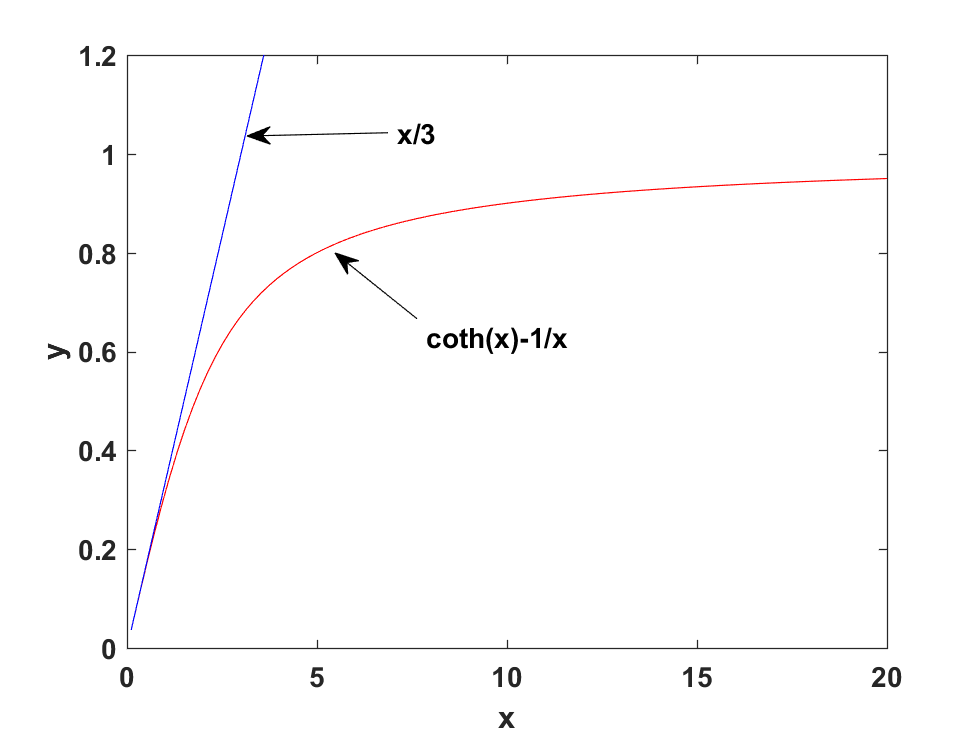
\includegraphics[width=8cm]{SUPG-curves.png}
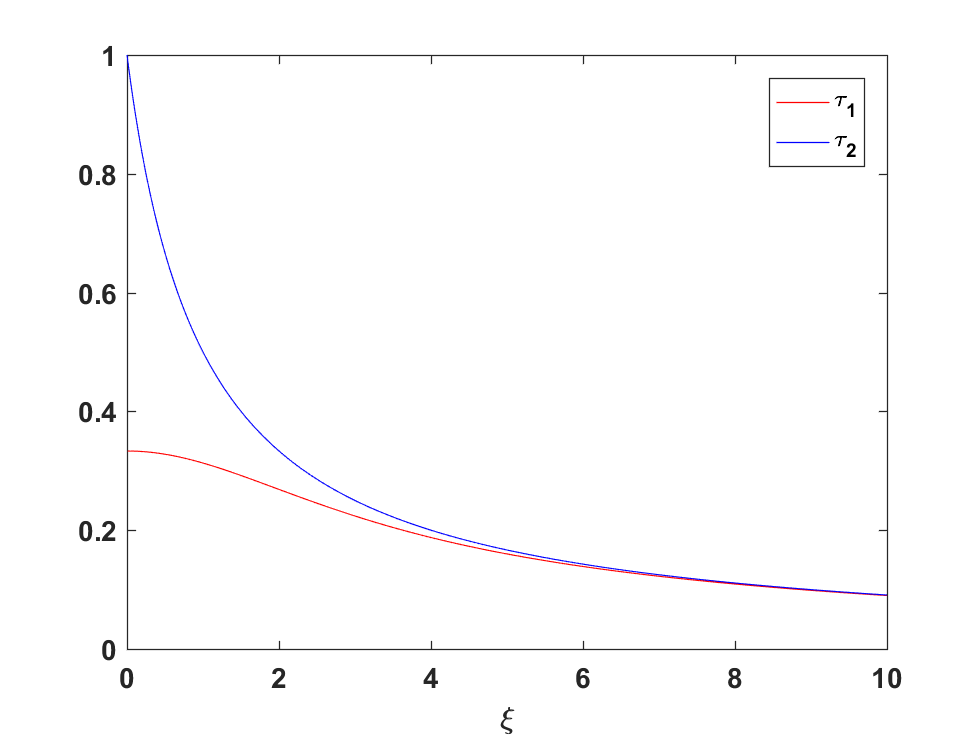
\includegraphics[width=8cm]{tau1tau2.png}
\caption{SUPG}
\label{fig:SUPG}
\end{figure}

A guidance as to how to select $\tau$ is looking at some specific
limits.  The SUPG correction term should vanish if $\Delta t \to 0$,
if $l\to 0$, and also if $|\bm{v}| \to 0$. A smart choice could then be
\[
\tau=\tau_1
\]
where
\begin{equation}
\tau_1 := \frac{l}{2 \, |\bm{v}|} \, \kappa 
\label{eq:UaSUPG}
\end{equation}
with 
\begin{equation}
\kappa=  \coth \xi - \frac{1}{\xi} 
\label{eq:kappa}
\end{equation}
where
\[
\xi=|\bm{v}| \, \Delta t/l
\]
is the element Courant number and $l$ is a characteristic local
element size.  For $\xi \ll 1$ we have $\kappa \sim \xi/3$, and
\[
\tau=\frac{l}{2 \, |\bm{v}|} \, \frac{| \bm{v} | \, \Delta t}{3 l} 
=\Delta t/6 
\]
hence
\[
M=\frac{\Delta t}{6} \bm{v} \cdot \nabla N
\]
showing that the perturbation term goes to zero as either
$\Delta t \to 0$ and $|\bm{v}| \to 0$. If $l \to 0$ then $\kappa \to 1$
and $\tau \to 0$, so all the above listed limits are obtained with
$\tau$ given by (\ref{eq:UaSUPG}). In summary, for $\tau=\tau_1$ given by (\ref{eq:UaSUPG}) we have
\[
M=\frac{l \kappa}{2 |\bm{v}|} \; \bm{v} \cdot \nabla N
\]
and the following limits
\begin{align}
M \to 0 &\quad \hbox{when} \quad \Delta t \to 0 \nonumber \\
M \to 0 &\quad \hbox{when} \quad  |\bm{v}| \to 0 \nonumber \\
M \to 0 &\quad \hbox{when} \quad  l \to 0 \nonumber \\
M \to \frac{l}{2} \frac{\bm{v}}{|\bm{v}|} \cdot \nabla N  &\quad \hbox{when} \quad \Delta t \to \infty \label{eq:tinf}\\
M \to \frac{l}{2} \frac{\bm{v}}{|\bm{v}|} \cdot \nabla N  &\quad \hbox{when} \quad |\bm{v}| \to \infty \label{eq:vinf} \\
M \to \frac{\Delta t}{6} \bm{v} \cdot \nabla N &\quad \hbox{when} \quad l \to \infty \label{eq:linf}
\end{align}

In the literature it is shown that (\ref{eq:tinf}) and (\ref{eq:vinf})
is the optimal choice in the convective limit, i.e.\ for large element
Courant numbers. Limit (\ref{eq:linf}) can be justified using
Taylor-Galerkin approach (see below).

The local element size, $l$, can be defined in a number of similar
ways leading to different numerical pre-factors to $\tau$ and
$\xi$. The exact functional relationship between $\kappa$ and $\xi$ is
also not uniquely defined.


Another option of creating a smooth transition between the temporal
and spatial criteria \ref{eq:tautemp} and \ref{eq:tauspacial} is to select $\tau$ as
\[
\tau=\tau_2
\]
where
\begin{equation}
  \tau_2:=\left ( \frac{1}{\tau_t} + \frac{1}{\tau_s} \right )^{-1}
\end{equation}
which can also be written as
\begin{equation}
  \tau_2:=\frac{1}{2} \frac{\Delta t}{1+ \xi}
\label{eq:tauswitch}
\end{equation}
Expression (\ref{eq:tauswitch}) gives the limits
\begin{align}
M \to 0 &\quad \hbox{when} \quad \Delta t \to 0 \nonumber \\
M \to 0 &\quad \hbox{when} \quad  |\bm{v}| \to 0 \nonumber \\
M \to 0 &\quad \hbox{when} \quad  l \to 0 \nonumber \\
M \to \frac{l}{2} \frac{\bm{v}}{|\bm{v}|} \cdot \nabla N  &\quad \hbox{when} \quad \Delta t \to \infty \nonumber\\
M \to \frac{l}{2} \frac{\bm{v}}{|\bm{v}|} \cdot \nabla N  &\quad \hbox{when} \quad |\bm{v}| \to \infty \nonumber \\
M \to \frac{\Delta t}{2} \bm{v} \cdot \nabla N &\quad \hbox{when} \quad l \to \infty \label{eq:linf2}
\end{align}
Apart from a different numerical factor in the last limit, all limits
are the same as obtained using definition (\ref{eq:UaSUPG}). 



Summarizing
\begin{align*}
  \tau_1 :=& \frac{l}{2 \, |\bm{v}|} \, \kappa  \\
  =& \frac{l}{2 \, |\bm{v}|} \,  ( \coth \xi - \frac{1}{\xi} )  \\
            =& \frac{l}{2 \, |\bm{v}|} \,  \left ( \coth \left (\frac{|\bm{v}| \, \Delta t}{l} \right ) - \frac{l}{|\bm{v}| \, \Delta t} \right ) 
\end{align*}
Since
\begin{align*}
  \frac{l}{2 | \bm{v} |} &= \frac{\Delta t}{2} \frac{l}{|\bm{v}| \Delta t} \\
                        &= \frac{\Delta t}{2} \frac{1}{\xi}
\end{align*}
These two above listed options for $\tau$ can also be written as
\begin{align}
\tau_1&=\frac{\Delta t}{2} \, \frac{1}{\xi} \left (\coth \xi - 1/\xi \right ) \label{eq:tau1} \\
\tau_2&=\frac{\Delta t}{2} \frac{1}{1+\xi} \label{eq:tau2}
\end{align}
and they are shown in Fig.~\ref{fig:SUPG}b as functions of $\xi$ for $\Delta t/2=1$. Only
for $|\bm{v}| \Delta t < 2 l$ is there any significant difference, and
the difference in newer larger than a factor 3 obtained in the limit
$\xi \to 0$.  It appears unlikely that there will be any significant
resulting differences between selecting $\tau=\tau_1$ or $\tau=\tau_2$
(see (\ref{eq:tau1}) and (\ref{eq:tau2})). Currently the SUPG
implementation in \Ua uses $\tau=\tau_1$.



Implementing SUPG implicitly using the $\Theta$ method leads to
\begin{align*}
0=  &<\rho (h_1-h_0)/\Delta t + (1-\Theta) (\nabla_{xy} \cdot \bm{q}_0  - a_0)  + \Theta (\nabla_{xy} \cdot \bm{q}_1  - a_1) , N  >\\
  + \beta   &<\rho (h_1-h_0)/\Delta t  + (1-\Theta) (  \nabla_{xy} \cdot q_0 -a_0)
  + \Theta (\nabla_{xy} \cdot \bm{q}_1 -a_1) , \tau \; ((1-\Theta) \bm{v}_0 +\Theta \bm{v}_1 ) \cdot \nabla_{xy} N  >
\end{align*}

Here the perturbation to the test-function space is a weighted average
over the values at the beginning and the end of the time step. This
adds another source of non-linearity to the problem. Experience showed
this to reduce the radius of convergence considerably and to increase
grumpiness on a personal level. Former can be avoided by using the
value of perturbation term at the beginning of the time step, i.e.\
\begin{align*}
0=  &<\rho (h_1-h_0)/\Delta t + (1-\Theta) (\nabla_{xy} \cdot \bm{q}_0  - a_0)  + \Theta (\nabla_{xy} \cdot \bm{q}_1  - a_1) , N  >\\
  & + \beta   <\rho (h_1-h_0)/\Delta t  +   \nabla_{xy} \cdot \bm{q}_0 -a_0 , \tau \; \bm{v}_0  \cdot \nabla_{xy} N  >
\end{align*}


% \section{SUPG stabilization}

% The mass conservation equaiton
% \[
%   \rho \p_t h +  \nabla_{xy} \cdot \bm{q} = \rho \, a 
% \]
% SUPG stabilization

% \[
% < \rho \p_t h + \nabla_{xy} \cdot \bm{q} - \rho a | N > + < \rho \p_t h + \nabla_{xy} \cdot \bm{q} - \rho a | \tau (\bm{v} \cdot \nabla_{xy} ) N > =0
% \]

% Since
% \begin{align*}
%   < \nabla_{xy} \cdot \bm{q} | \tau (\bm{v} \cdot \nabla_{xy} ) N >
%   & = < \nabla_{xy} \cdot \bm{q} | \tau (\bm{v} \cdot \nabla_{xy} ) N > \\
%   & = < \nabla_{xy} \cdot (h \bm{v}) | \tau (\bm{v} \cdot \nabla_{xy} ) N > \\
%   & = < \bm{v} \cdot \nabla_{xy} h + h \nabla_{xy} \cdot \bm{v} | \tau (\bm{v} \cdot \nabla_{xy} ) N > \\
%   & = < \bm{v} \cdot \nabla_{xy} h | \tau (\bm{v} \cdot \nabla_{xy} ) N >   + < h \nabla_{xy} \cdot \bm{v} | \tau (\bm{v} \cdot \nabla_{xy} ) N > \\
% % \end{align*}


\section{SIA-motivated diffusion}
\[
\bm{q}= \bm{q}^b+\bm{q}^d
\]
where
\[
\bm{q}^b=\bm{v} h
\]
and
\[
\bm{q}^d= \rho \, D h^{n+2} \; | \nabla_{xy} s |^{n-1} \,  \nabla s 
\]
where
\[
D=\frac{2A}{n+2} (\rho g)^n 
\]


\[
s= (h+B) \He(h-h_f)+ (1-\He(h-h_f)) (S+(1-\rho/\rho_o)\; h )
\]
and therefore (almost)
\[
\p_x s= (\p_x h+ \p_x B) \He(h-h_f)+ (1-\He(h-h_f)) (S+(1-\rho/\rho_o)\; \p_x h )
\]

This motivates adding a SIA based diffusion term
\[
-D <| \nabla_{xy} s | ^{n-1} \, h^{n+2} \nabla s | \nabla_{xy} N >
\]
However, this is (currently) not done in \Ua.

In 1HD the SIA form of the continuity equation can be written as
\[
 \rho \p_t s + \p_x ( k \p_x s) = \rho a
\]
with 
\[
k:= \frac{2 \rho A (\rho g)^n }{n+2}  |\p_x s|^{n-1} h^{n+2}    
\]

suggesting a Peclet number
\[
\mathrm{Pe}= \frac{u L}{k} 
\]


\section{Connection between third order Taylor-Galerkin (TG3) and  streamline-upwind Petrov-Galerkin (SUPG)}

In the context of SUPG, the TG3 system given by (\ref{eq:TG3i}) can be
thought of as also introducing extra weighting term beside the
standard $N$ term. But those additional weighting terms are only
applied to the source term ($a$) and the spatial term, and not to the
time-derivative term. Furthermore, as mentioned above in a steady-state these extra
weighting terms cancel each other out.



It is instructive to consider as well the case where a second-order forward Taylor expansion
\begin{equation}
h_1=h_0+ \Delta t \, \p_t h_0 + \frac{(\Delta t)^2}{2} \p^2_{tt} h_0 
\label{eq:t2f}
\end{equation}
is used instead of the centred expansion given by  Eq.~(\ref{eq:three}).
Inserting (\ref{eq:mass}) and (\ref{eq:qv}) into (\ref{eq:t2f}) gives
\[
0=h_1- h_0 - \Delta t \, (a -  \nabla_{xy} \cdot \bm{q}) - \frac{(\Delta t)^2}{2} (\p_t a-  \nabla_{xy} \cdot ( \bm{v} (a-\nabla_{xy} \cdot \bm{q}) + h \, \p_t \, \bm{v}))
\]
The Galerkin system is
\begin{align*}
<\rho(h_1-h_0),N> &=\Delta t \, <\rho a -  \nabla_{xy} \cdot \bm{q},N> \nonumber \\
+&\frac{(\Delta t)^2}{2} <\rho \p_t a ,N> - \frac{(\Delta t)^2}{2} <\rho \, h \,\p_t \bm{v}, N> \nonumber \\
+& \frac{(\Delta t)^2}{2} <  \rho a-\nabla_{xy} \cdot \bm{q} , \bm{v} \cdot \nabla_{xy} N>
\end{align*}
where a partial integration has been used to get rid of second order
derivatives (not writing the boundary terms). The last term is similar
to what in some other ad-hoc methods is introduced as a stabilisation
term. This term only acts in the direction of flow and is zero
transverse to the flow direction.  In the above expression all terms
are to be evaluated at the beginning of the interval. This approach is
usually referred to as the second-order explicit Taylor-Galerkin (TG2e)
method. If we evaluate all terms by taking the mean value over the
time interval, we get an implicit method, but now the second-order
terms do not cancel out in steady-state, and the resulting method is
quite similar to the streamline-upwind Petrov-Galerkin.

Dropping the time derivatives of $a$ and $\bm{v}$, we can rewrite the above system as
\[
<\rho(h_1-h_0)/\Delta t,N> =<\rho a -  \nabla_{xy} \cdot \bm{q},N + \frac{1}{2} \Delta t \; \bm{v} \cdot \nabla_{xy} N > 
\]
showing that the TG2e results in an `inconsistent' weighting with $\tau=\Delta t$ and $\beta=1/2$.  



Comparing \ref{eq:TG3i} with (\ref{eq:SUPG1}), TG3 can  be
interpreted as a some sort of Petrov-Galerkin method where only the
spatial terms and the source terms are multiplied by a modified test
function. In  TG3 the modified test function
is
\begin{equation}
N+ \frac{\Delta t}{6}  \; \bm{v} \cdot \nabla_{xy} N,
\label{eq:t3}
\end{equation}
wheres in SUPG it has the form
\begin{equation}
N+ \beta \tau  \; \bm{v} \cdot \nabla_{xy} N .
\label{eq:t4}
\end{equation}
The weighting is done inconsistently in TG3, i.e.\ not over the
time-derivative. Apart for the inconsistent weighting used in TG3,
the SUPG is equal to TG3 provided the two adjustable parameters
$\beta$ and $\tau$ are selected as $\beta=1/6$ and $\tau=\Delta t$.


The TG3 methods follows automatically from a third-order Taylor
expansion and involves no adjustable parameters. The SUPG is in
essence a heuristic method.


\section{Implementing fully-implicit}

In a fully implicit approach using the Newton-Raphson iteration the unknowns at time-step 1 are written in incremental form as
\begin{align*}
u^{i+1}_1&=\Delta u + u^i_1, \\
v^{i+1}_1&=\Delta v + v^i_1, \\
h^{i+1}_1&=\Delta h + h^i_1, \\
\end{align*}
where $u^{i+1}_1$ is the estimate for $u_1$ at Newton-Raphson
iteration step $i$. (Note that $\Delta h \not = h_1-h_0$ and that
$\Delta h \to 0$ with increasing $i$.)



\subsection{First-order fully implicit}
Taking only the first-order Taylor terms from \eqref{eq:uvhT3G}, and
only considering the $x$ components for the time being, gives
\begin{align*}
0&=\frac{\rho}{\Delta t} (\Delta h + h^i_1-h_0) \\
&- \frac{1}{2}(\rho(a_0+a_1)-\p_x(\rho u_0 h_0)-\p_x(\rho (\Delta h + h^i_1) (\Delta u + u^i_1)))
\end{align*}

If the specific mass balance is a function of thickness, i.e.
\[
a=a(h)
\]
then an additional term must be added to the matrix on the left-hand
side, and the right-hand side terms must be evaluated within the NR
loop every time that the thickness is updated. The first-order equation is then 
\begin{align*}
0&=\frac{\rho}{\Delta t} (\Delta h + h^i_1-h_0) \\
&- \frac{1}{2}\left (\rho \left (a_0(h_0)+a_1(h_1)+ \p_h a_1|_{h_1} \, \Delta h \right )-\p_x(q_{x0})-\p_x((\Delta h + h^i_1)) (\Delta u + u^i_1) \right )
\end{align*}

Ignoring second-order terms and taking the terms involving the unknown
$\Delta h$ to the left-hand side leads to
\begin{align}
\label{eq:fTG}
\rho \frac{\Delta h}{\Delta t}
&+ \frac{1}{2}\left ( \p_x(\rho u^i_1 \, \Delta h  + \rho h^i_1 \,\Delta u ) + \p_y (\rho v^i_1 \, \Delta h  + \rho h^i_1 \,\Delta v )
- \rho \p_h a |_{h_1}\, \Delta h)\right ) \\
  &=\frac{\rho}{2}(a_0+a_1)-\frac{\rho}{\Delta t}  (h^i_1-h_0)- \frac{1}{2}(\p_x(q_{x0})+\p_x(\rho h^i_1 u^i_1) + \p_y(q_{0y})+\p_y(\rho h^i_1 v^i_1))
\nonumber
\end{align}
where the corresponding $y$ terms have been added.




\subsection{Fully implicit SSTREAM time integration with the $\Theta$ method}


\[
\mathrm{K}^{uu}\, \Delta \bm{u} :=D \bm{r}_x(\bm{u}_1^{i},\bm{v}_1^i,\bm{h}_1^i)[\Delta \bm{u}]
\]


\begin{equation}
\left [ \begin{array}{ccc}
      \mathrm{K}^{uu} &  \mathrm{K}^{uv} & \mathrm{K}^{uh} \\
      \mathrm{K}^{vu} &  \mathrm{K}^{vv} & \mathrm{K}^{vh} \\
      \mathrm{K}^{hu} &  \mathrm{K}^{hv} & \mathrm{K}^{hh} \\
\end{array} \right ]
\left [ \begin{array}{c}
       \Delta \bm{u} \\
       \Delta \bm{v} \\
       \Delta \bm{h} 
\end{array} \right ]
=\left [ \begin{array}{c} 
\bm{r}_u \\ 
\bm{r}_v  \\
\bm{r}_h 
\end{array} 
\right ]
\end{equation}


We go from time step $t=t_0$ to $t=t_1$ and solve for the unknown values for $\bm{u}$,
$\bm{v}$, and $\bm{h}$, at $t=t_1$ ($\bm{u}_1$, $\bm{v}_1$, and $\bm{h}_1$)
given their respective values at $t=t_0$ ($\bm{u}_0$, $\bm{v}_0$, and $\bm{h}_0$).

\begin{eqnarray*}
\bm{u}_1^{i+1}&=& \bm{u}_1^{i}+ \Delta \bm{u} \\
\bm{v}_1^{i+1}&=& \bm{v}_1^{i}+ \Delta \bm{v} \\
\bm{h}_1^{i+1}&=& \bm{h}_1^{i}+ \Delta \bm{h} 
\end{eqnarray*}



For notational simplicity we omit the $i$ superscript and it is to be understood that the values of
$\eta$, $\beta^2$, $h$, $u$, and $v$ are the estimated values at iteration $i$.

At element level the matrices are
\begin{eqnarray*}
[\mathrm{K}^{uu}]_{pq} 
&=&\int_{\Omega} \big \{
4 \eta h \p_x N_p \,\p_x N_q  + h \eta \p_y N_p \, \p_y N_q 
+ \He(h-h_f) \beta^2 N_p N_q \\
& & + h D_{eu} (4 \p_x u + 2 \p_y v) \, \p_x N_p+ h D_{eu} (\p_x v + \p_y u) \, \p_y N_p \\
& & + D_b\, u \, u \,N_p \, N_q \big \} \, dx \, dy
\end{eqnarray*}


\begin{eqnarray*}
[\mathrm{K}^{vv}]_{pq} 
&=&\int_{\Omega}  \big \{
4 \eta h \p_y N_p \, \p_y N_q  + h \eta \p_x N_p \, \p_x N_q 
+ \He(h-h_f) \beta^2 N_p N_q \\
& & + h D_{ev} (4 \p_y v + 2 \p_x u) \, \p_y N_p + h D_{ev} (\p_x v + \p_y u) \, \p_x N_p \\
& & + D_b\, v \, v \,N_p \, N_q \big \} \, dx \, dy
\end{eqnarray*}



\begin{eqnarray*}
[\mathrm{K}^{uv}]_{pq}  
&=&\int_{\Omega} \big \{
h \eta ( 2 \p_x N_p \,\p_y N_q+ \p_y N_p \, \p_x N_q) \\
& & + h D_{ev} (4 \p_x u + 2 \p_y v) \, \p_x N_p + h D_{ev} (\p_x v + \p_y u) \, \p_y N_p \\
& & + D_b\, u \, v \,N_p \, N_q \big \} \, dx \, dy
\end{eqnarray*}


    %     
\begin{eqnarray*}
[\mathrm{K}^{uv}]_{pq} 
&=&\int_{\Omega} \big \{
h \eta ( 2\p_y N_p \, \p_x N_q+ \p_x N_p \, \p_y N_q) \\
& & + h D_{eu} (4 \p_y v + 2 \p_x u) \, \p_y N_p + h D_{eu} (\p_x v + \p_y u) \, \p_x N_p \\
& & + D_b\, u \, v \,N_p \, N_q \big \} \, dx \, dy
\end{eqnarray*}

(floating only (original version)
\begin{eqnarray*}
[\mathrm{K}^{xh}]_{pq} 
&=&\int_{\Omega} \big \{
\eta ( 4 \p_x u + 2 \p_y v) \p_x N_p \, N_q+ \eta (\p_y u + \p_x v) \, \p_y  N_p \, N_q \\
& & + \delta(h-h_f) \beta^2 u N_p \, N_q\\
& & + \rho g ( \He(h-h_f) + h \delta(h-h_f))\, (( \rho /\rho_o \p_x h- \p_x H) \cos \alpha  -  \sin \alpha ) N_p N_q   \\
& & + \frac{\rho^2 g}{\rho_o}  h \He(h-h_f)  \, \cos \alpha \, N_p \, \p_x N_q    \\
& & -\varrho g h \cos \alpha \,\p_x N_p \, N_q \big \} \, dx \, dy
\end{eqnarray*}
)


(floating only (corrected July 2011)
\begin{eqnarray*}
[\mathrm{K}^{xh}]_{pq} 
&=&\int_{\Omega} \big \{
\eta ( 4 \p_x u + 2 \p_y v) \p_x N_p \, N_q+ \eta (\p_y u + \p_x v) \, \p_y  N_p \, N_q \\
& & + \delta(h-h_f) \beta^2 u N_p \, N_q\\
& & + \rho g  \He(h-h_f) \, (( \rho /\rho_o \p_x h- \p_x H) \cos \alpha  -  \sin \alpha ) N_p N_q   \\
& & + \frac{\rho^2 g}{\rho_o}  h \He(h-h_f)  \, \cos \alpha \, N_p \, \p_x N_q    \\
& & + \frac{\rho^2}{\rho_o} \delta(h-h_f) \, \cos \alpha \, h\,\p_x h \, N_p \, N_q\\
& & -\varrho g h \cos \alpha \,\p_x N_p \, N_q \big \} \, dx \, dy
\end{eqnarray*}
)



(general case
\begin{align*}
[\mathrm{K}^{uh}]_{pq} 
&=\int_{\Omega} \big \{
\eta ( 4 \p_x u + 2 \p_y v) \p_x N_p \, N_q+ \eta (\p_y u + \p_x v) \, \p_y  N_p \, N_q \\
&  + \delta(h-h_f) \beta^2 u N_p \, N_q\\
& +   \rho g \He(h-h_f)  \, \p_x B \, \cos \alpha \, N_p \, N_q  -  \rho g \sin \alpha  N_p \,N_q   \\
& - \rho g h \left ( 1 - \frac{\rho}{\rho_o} \He(h_f-h)  \right ) \, \cos \alpha \, \p_x N_p \,  N_q    \\
\end{align*}
)


( floating only version:
\begin{eqnarray*}
[\mathrm{K}^{vh}]_{pq} 
&=&\int_{\Omega} \big \{
\eta ( 4 \p_y v + 2 \p_x u) \p_y N_p \, N_q+ \eta (\p_x v + \p_y u) \,\p_x  N_p \,N_q \\
& & + \delta(h-h_f) \beta^2 v N_p \, N_q\\
& & + \rho g ( \He(h-h_f) + h \delta(h-h_f)) \,( \rho /\rho_o \p_y h- \p_y H) \cos \alpha \, N_p N_q   \\
& & + \frac{\rho^2 g}{\rho_o}  h \He(h-h_f)  \, \cos \alpha \, N_p \, \p_y N_q    \\
& & -\varrho g h \cos \alpha \,\p_y N_p \, N_q \big \} \, dx \, dy
\end{eqnarray*}
)

( general case
\begin{eqnarray*}
[\mathrm{K}^{vh}]_{pq} 
&=&\int_{\Omega} \big \{
\eta ( 4 \p_y v + 2 \p_x u) \p_y N_p \, N_q+ \eta (\p_x v + \p_y u) \,\p_x  N_p \,N_q \\
& & + \delta(h-h_f) \beta^2 v N_p \, N_q\\
& & + \rho g ( \He(h-h_f) + h \delta(h-h_f)) \,( \rho /\rho_o \p_y h- \p_y H) \cos \alpha \, N_p N_q   \\
& & + \frac{\rho^2 g}{\rho_o}  h \He(h-h_f)  \, \cos \alpha \, N_p \, \p_y N_q    \\
& & -\varrho g h \cos \alpha \,\p_y N_p \, N_q \big \} \, dx \, dy
\end{eqnarray*}
)



\begin{eqnarray} 
[\mathrm{K}^{hu}]_{pq} &=& \theta (\p_x h \, N_q + h \, \p_x N_q )  \, N_p \nonumber 
\end{eqnarray}
\begin{eqnarray} 
[\mathrm{K}^{hv}]_{pq} &=& \theta (\p_y h \, N_q + h \, \p_y N_q ) \, N_p \nonumber 
\end{eqnarray}


\begin{eqnarray} 
[\mathrm{K}^{hh}]_{pq} &=& (N_q/\Delta t 
+ \theta (\p_x u \, N_q + u \p_x N_q + \p_y v \, N_q + v \p_y N_q )) \, N_p
\nonumber 
\end{eqnarray}




In the equations the quantities $D_{eu}$, $D_{ev}$, $E$, and $D_b$, which arise because of the
linearisation of $\eta$ and $\beta^2$, are given by
\begin{eqnarray}
D_{eu} &=& E ((2 \p_x u + \p_y v) \p_x N_q + \frac{1}{2} (\p_x v + \p_y u) \p_y N_q )\\
D_{ev} &=& E ((2 \p_y v + \p_x u) \p_y N_q + \frac{1}{2} (\p_x v + \p_y u) \p_x N_q )\\
\end{eqnarray}

\[ 
   E= \frac{1-n}{4 n} A^{-1/n} \dot{\epsilon}^{(1-3n)/n}
\]

\[
D_b:=(1/m-1) \, C^{-1/m} \, |\bm{v}|^{(1-3m)/m}
\]



\subsubsection{Third-order Taylor-Galerkin fully implicit}

The terms in
\begin{align}
& \frac{\Delta t^2}{12} \int (  \p_t a_1 N + ( h_1 \p_t u_1 + u_1 (a_1-\p_x (q_{x1})-\p_y (q_{y1}))) \p_x N \nonumber \\
&  \hspace{2.4cm}  + ( h_1 \p_t v_1 + v_1 (a_1-\p_x (q_{x1})-\p_y (q_{y1})))\p_y N )\, dA \nonumber \\
\end{align}
from \eqref{eq:uvhT3G}, need to be linearised. Starting with
\[
   h_1 \p_t u_1 + u_1 (a_1-\p_x (q_{x1})-\p_y (q_{y1})) 
\]
and and inserting $h^{i+1}=\Delta h + h^i_1$ etc.\ gives
\begin{align*}
 (\Delta h + h^i_1) \p_t(\Delta u + u^i_1) 
+(\Delta u + u^i_1) (a_1-\p_x ((\Delta h + h^i_1)(\Delta u + u^i_1))-\p_y ((\Delta h + h^i_1) (\Delta v + v^i_1))
\end{align*}
and first ignoring only some second-order terms 
\begin{align*}
 \p_t u^i_1\,  \Delta h + h^i_1 \, \p_t \Delta u `+ h^i_1 \p_t u^i_1
+(a_1 \, \Delta u  + u^i_1 a_1 ) 
- (\Delta u + u^i_1)  (\p_x (u^i_1 \, \Delta h + h^i_1\,\Delta u + h^i_1 u^i_1)+\p_y (v_1 \, \Delta h + h^i_1 \, \Delta v+h^i_1 v^i_1))
\end{align*}
and then ignoring the remaining second-order terms
\begin{align*}
 ((u^i_1-u_0)/\Delta t) (\Delta h + h^i_1) 
&+a_1 \, \Delta u  + u^i_1 a_1 \\
&- u^i_1  (\p_x (u^i_1 \, \Delta h + h^i_1\,\Delta u + h^i_1 u^i_1)+\p_y (v_1 \, \Delta h + h^i_1 \, \Delta v+h^i_1 v^i_1)) \\
&- ( \p_x (h^i_1 u^i_1) +\p_y (h^i_1 v^i_1)) \, \Delta u
\end{align*}
where $\p_t u^i_1=(u^i_1-u_0)/\Delta t$ and $\p_t \Delta u$ has been set to zero. Now shifting the unknowns over to the left-hand side
\begin{align*}
& \p_t u^i_1 \, \Delta h + a_1 \, \Delta u \\
&- u^i_1  (\p_x (u^i_1 \, \Delta h + h^i_1\,\Delta u ) +\p_y (v_1 \, \Delta h + h^i_1 \, \Delta v)) \\
&- ( \p_x (h^i_1 u^i_1) +\p_y (h^i_1 v^i_1)) \, \Delta u \\
&=  u^i_1  (\p_x( h^i_1 u^i_1)+\p_y (h^i_1 v^i_1)) - u^i_1 a_1 -\p_t u^i_1 \,h^i_1 
\end{align*}
and adding the $y$ terms
\begin{align*}
& (\p_t u^i_1 \p_x N +\p_t v^i_1 \p_y N ) \Delta h  + a_1 \, (\p_x N \, \Delta u  + \p_y N \, \Delta v) \\
&- (u^i_1 \p_x N +v^i_1 \p_y N )  (\p_x (u^i_1 \, \Delta h + h^i_1\,\Delta u ) +\p_y (v_1 \, \Delta h + h^i_1 \, \Delta v)) \\
&- ( \p_x (h^i_1 u^i_1) +\p_y (h^i_1 v^i_1)) \, (\p_x N \, \Delta u+\p_y N \, \Delta v)\\
=&  (\p_x N \, u^i_1+\p_y N \, v^i_1) \,  (\p_x( h^i_1 u^i_1)+\p_y (h^i_1 v^i_1)) -a_1 (\p_x N \, u^i_1 +\p_y N \, v^i_1) -(\p_t u^i_1 \p_x N + \p_t v^i_1 \p_x N) \,h^i_1 
\end{align*}
Then adding the remaining higher-order Taylor terms in \eqref{eq:uvhT3G},
involving fields from time-step zero,  to the right-hand side gives
\begin{align*}
& (\p_t u^i_1 \p_x N +\p_t v^i_1 \p_y N ) \, \Delta h  \\
&+  (\p_x N \, \Delta u+\p_y N \, \Delta v) \, (a_1- \p_x (h^i_1 u^i_1) +\p_y (h^i_1 v^i_1))  \\
&- (\p_x N \, u^i_1    +\p_y N \, v^i_1 )  \, (\p_x (u^i_1 \, \Delta h + h^i_1\,\Delta u ) +\p_y (v_1 \, \Delta h + h^i_1 \, \Delta v)) \\
=& \p_t (a_0-a_1) N \\
&-  ( u^i_1 \,\p_x N + v^i_1 \, \p_y N)   (a_1- \p_x ( h^i_1 u^i_1)+\p_y (h^i_1 v^i_1))  - h^i_1 \, (\p_t u^i_1 \, \p_x N + \p_t v^i_1 \, \p_y N)  \\
&+  (u_0   \,\p_x N + v_0  \,  \p_y N)   (a_0 - \p_x ( q_{x0} ) + \p_y  (q_{0y} )  )   + h_0   \,  (\p_t u_0   \, \p_x N + \p_t v_0 \, \p_y N) 
\end{align*}
Now adding first-order Taylor terms from \eqref{eq:fTG} to the expression above

\begin{align*}
\Delta h  \, N&+ \frac{\Delta t}{2}\left ( \p_x(u^i_1 \, \Delta h  + h^i_1 \,\Delta u ) + \p_y (v^i_1 \, \Delta h  + h^i_1 \,\Delta v ) \right ) N\\
&+ \gamma (\p_t u^i_1 \p_x N +\p_t v^i_1 \p_y N ) \, \Delta h  \\
&+  \gamma (\p_x N \, \Delta u+\p_y N \, \Delta v) \, (a_1- \p_x (h^i_1 u^i_1) +\p_y (h^i_1 v^i_1))  \\
&- \gamma (\p_x N \, u^i_1    +\p_y N \, v^i_1 )  \, (\p_x (u^i_1 \, \Delta h + h^i_1\,\Delta u ) +\p_y (v_1 \, \Delta h + h^i_1 \, \Delta v)) \\
=&\left ( h_0-h^i_1+\frac{\Delta t}{2}(a_0+a_1)- \frac{\Delta t}{2}(\p_x(q_{x0})+\p_x(h^i_1 u^i_1) + \p_y(q_{0y})+\p_y(h^i_1 v^i_1))  \right ) N\\
&+ \gamma \p_t (a_0-a_1) N \\
&-  \gamma ( u^i_1 \,\p_x N + v^i_1 \, \p_y N)   (a_1- \p_x ( h^i_1 u^i_1)+\p_y (h^i_1 v^i_1))  - \gamma h^i_1 \, (\p_t u^i_1 \, \p_x N + \p_t v^i_1 \, \p_y N)  \\
&+  \gamma(u_0   \,\p_x N + v_0  \,  \p_y N)   (a_0 - \p_x ( q_{x0} ) + \p_y  (q_{0y} )  )   + \gamma h_0   \,  (\p_t u_0   \, \p_x N + \p_t v_0 \, \p_y N) 
\end{align*}


which can also be written as
\begin{align*}
\Delta h  \, N &+ 
\left (\kappa \,N - \gamma \,(\p_x N \, u^i_1    +\p_y N \, v^i_1 ) \right ) 
\left ( \p_x(u^i_1 \, \Delta h  + h^i_1 \,\Delta u ) + \p_y (v^i_1 \, \Delta h  + h^i_1 \,\Delta v ) \right ) \\
&+ \gamma (\p_t u^i_1 \p_x N +\p_t v^i_1 \p_y N ) \, \Delta h  \\
&+  \gamma (\p_x N \, \Delta u+\p_y N \, \Delta v) \, (a_1- \p_x (h^i_1 u^i_1) -\p_y (h^i_1 v^i_1))  \\
=&  ( h_0-h^i_1) \, N \\
&+ \left (\kappa \, N+ \gamma(u_0 \, \p_x N + v_0 \, \p_y N) \right )   \left ( a_0 -\p_x(q_{x0})- \p_y(q_{0y}))  \right ) \\
&+ \left (\kappa\, N-\gamma (u^i_1 \, \p_x N + v^i_1 \, \p_y N) \right ) \left ( a_1 -\p_x(h^i_1 u^i_1) -\p_y(h^i_1 v^i_1))  \right ) \\
&+ \gamma \p_t (a_0-a_1) N \\
&- \gamma h^i_1 \, (\p_t u^i_1 \, \p_x N + \p_t v^i_1 \, \p_y N)  \\
&+ \gamma h_0   \,  (\p_t u_0   \, \p_x N + \p_t v_0 \, \p_y N) 
\end{align*}


where
\[
\gamma=\frac{(\Delta t)^2}{12} 
\]
and
\[
\kappa=\frac{\Delta}{2}
\]




\subsection{Semi-implicit: $uv$ explicit, and $h$ implicit}
In the semi-implicit approach $h_1$ is treated as the unknown while
$h_0$, $u_1$, $v_1$, $h_0$, $v_0$ are assumed to be known.  


Taking the unknown $h_1$ in \eqref{eq:uvhT3G} to the left-hand side gives
\begin{align*}
\lefteqn{\int( h_1 + \frac{\Delta t}{2}( \p_x(q_{x1} ) + \p_y(q_{y1} ))) \,N\, dA }\\
&+ \frac{\Delta t^2}{12} \int (( h_1 \p_t u_1 - u_1 (\p_x (q_{x1})+\p_y (q_{y1}))) \p_x N +  (h_1 \p_t v_1 - v_1 (\p_x (q_{x1})+\p_y (q_{y1})))\p_y N )\, dA \\
&- \frac{\Delta t^2}{12} \oint (( h_1 \p_t u_1 - u_1 (\p_x (q_{x1})+\p_y (q_{y1}))) n_x + ( h_1 \p_t v_1 - v_1 (\p_x (q_{x1})+\p_y (q_{y1}))) n_y )\, N \, d\gamma\\
&=\int( h_0 + \frac{\Delta t}{2} (a_0 +a_1 -\p_x( q_{x0}) -\p_y ( q_{0y}) ))\,N\, dA \\
&+ \frac{\Delta t^2}{12} \int (  \p_t (a_0-a_1) N +( h_0 \p_t u_0 -u_1 a_1 + u_0 (a_0-\p_x (q_{x0})-\p_y (q_{0y}))) \p_x N \\
&  \hspace{3.3cm} +( h_0 \p_t v_0  -v_1 a_1 +v_0 (a_0-\p_x (q_{x0})-\p_y (q_{0y})))\p_y N )\, dA\\
&- \frac{\Delta t^2}{12} \oint (( h_0 \p_t u_0 -u_1 a_1 + u_0 (a_0-\p_x (q_{x0})-\p_y (q_{0y}))) n_x \\
&  \hspace{1cm} +( h_0 \p_t v_0 -v_1 a_1 + v_0 (a_0-\p_x (q_{x0})-\p_y (q_{0y}))) n_y )\, N \,d\gamma
\end{align*}



\section{Transient implicit SSHEET/SIA with the $\Theta$ method}

An implicit method us used where $h_0$ and $h_1$ are the ice
thicknesses at the beginning and the end of the time step,
respectively.  The system is solved using NR, and we write
\begin{align*}
 h^{i+1}&=h^i+\Delta h\\ 
 s^{i+1}&=s^i+\Delta h
\end{align*}
where $i$ is the number of the non-linear iteration step. Provided the method converges, $\Delta h$ goes to zero with
increasing $i$. In the following we simply write $h$ instead of $h^i$.

\[
(h+\Delta h -h_0)/\Delta t=-(1-\Theta) \nabla_{xy} \cdot \bm{q}_0 -  \Theta \nabla_{xy} \cdot \bm{q}_1(h+\Delta h)
\]


\begin{equation}
\int_{\Omega} (h+\Delta h -h_0) N \Omega= -(1-\Theta) \Delta t \int_{\Omega} N \nabla_{xy} \cdot \bm{q}_0 -  \Theta \Delta t \int_{\Omega} N \nabla_{xy} \cdot \bm{q}_1(h+\Delta h)
\label{eq:hvar}
\end{equation}

To use the above equation we need to know the perturbation in flux due
to perturbation in thickness.


The simplest way of perturbing $q(h)$ with respect to $h$ is to find
\[
\delta q = \lim_{\eps \to 0} \frac{d}{d\eps} q(h+\eps \Delta h).
\]



As using SSHEET for floating ice shelves is somewhat questionable we
here only consider the case of grounded ice\footnote{In general the
  surface is related tho the ice thickness and bed through
\[
s=(h+B) \He(h-h_f)+(S+(1-\rho/\rho_o) h) \, \He(h_f-h).
\]}. Where grounded
\[
q_x(h)=-\rho \, D \left ((\p_x h+ \p_x B)^2+(\p_y h+\p_y B)^2 \right )^{(n-1)/2} \; h^{n+2} \; \p_x s,
\]
and 
\[
\Delta s= \Delta h,
\]
with 
\[
D=\frac{2 A}{n+2} (\rho g)^n 
\]

Therefore
\begin{align*}
\delta q_x & = \lim_{\eps \to 0} \frac{d}{d\eps} q_x(h+\eps \Delta h)\\
            &= - D \, \lim_{\eps \to 0} \frac{d}{d\eps} D \left ( \p_x (s+\eps \Delta h)^2 + \p_y (s+\eps \Delta h)^2 \right )^{(n-1)/2} \; (h+\eps \Delta h)^{n+2} \; \p_x (s+\eps \Delta h)\\
            &= - D \, |\nabla_{xy}s |^{n-1} \, h^{n+2} \; \p_x \Delta h \\
            &\quad - D \, (n+2) |\nabla_{xy} s|^{n-1} \; h^{n+1} \, \p_x s \; \Delta h \\
            &\quad - D \,(n-1) |\nabla_{xy} s|^{n-3}  \left ( \p_x s \, \p_x \Delta h + \p_y s \, \p_y \Delta h \right )  \; h^{n+2} \, \p_x s
\end{align*}

The first term of the final expression shown above is the perturbation
in flux due to increase in slope, the second one the perturbation due
to increase in thickness. The third term is non-linear terms that
vanishes for $n=1$. This third term represents changes flux caused by
a change in effective viscosity due to perturbations in slope. This third 
terms shows that a change in slope in $y$ direction gives rise to an
increase in flux in $x$ direction.

As expected, for a negative unperturbed surface slope ($\p_x s < 0$),
both a positive perturbation in thickness ($\Delta h>0)$, and an
increase in (negative) surface slope ($\p_x \Delta h <0 $), result in a
positive perturbation in flux ($\delta q_x>0$).

\subsection{SSHEET with no-flux natural boundary condition}
Using a variant of Gauss theorem given by Eq.~(\ref{eq:fgg}) we write (\ref{eq:hvar}) on the form
\begin{equation}
\int_{\Omega} N \nabla_{xy} \cdot \bm{q} \; d \Omega = \oint_{\p \Omega} N \bm{q} \cdot \hat{\bm{n}} \, d \Gamma - \int_{\Omega} \nabla_{xy} N \cdot \bm{q} \, d \Omega 
\label{eq:gg}
\end{equation}
Applying (\ref{eq:gg}) on (linearised) (\ref{eq:hvar}) and assuming
that $\bm{q} \cdot \hat{\bm{n}}=0$ on $\p \Omega$, i.e.\ ice flux
across the boundary is zero (homogeneous Neumann boundary condition),
gives
\begin{align*} 
\int_{\Omega}  (h+\Delta h - h_0) \, N \; d \Omega 
   =& (1-\Theta) \Delta t \int \bm{q}_0 \cdot \nabla_{xy}  N \; d \Omega \\ 
   &+  \Theta \Delta t \int \bm{q}_1^i \cdot \nabla_{xy} N \; d \Omega \\ 
   &+ \Theta \Delta t \int \Delta \bm{q} \cdot  \nabla_{xy} N \; d \Omega 
\end{align*}
or
\begin{align*} 
\int_{\Omega}  \Delta h  \, N \; d \Omega &- \Theta \Delta t \int_{\Omega} \Delta \bm{q} \cdot  \nabla_{xy} N \; d \Omega \\
    =& - \int_{\Omega}  (h-h_0) \, N \; d \Omega  \\
    &+ (1-\Theta) \Delta t \int_{\Omega} \bm{q}_0 \cdot \nabla_{xy}  N \; d \Omega \\ 
    &+  \Theta \Delta t \int_{\Omega} \bm{q}_1^i \cdot \nabla_{xy} N \; d \Omega 
\end{align*}
where $\bm{q}^{i+1}=\bm{q}^i+\Delta \bm{q}$ is the NR iteration, with
\begin{align*}
\Delta q_x       = & - D(n-1) h^{n+2} |\nabla_{xy} s|^{n-3} \p_x s ( \p_x s \,\p_x \Delta h + \p_y s \,\p_y \Delta h))  \\
                   & - D(n+2) |\nabla_{xy} s|^{n-1} h^{n+1} \, \p_x s \; \Delta h \\
                   & - D|\nabla_{xy}s |^{n-1} \, h^{n+2} \; \p_x \Delta h
\end{align*}
Collecting terms, and writing $s$ and $h$ instead of $s^{i+1}$ and $h^{i+1}$, respectively, and 
$s_0$ and $h_0$ instead of $s^{i}$ and $h^{i}$, gives
\begin{align*}
&\int N_p N_q \; \Delta h_q \; d \Omega \\
+\Theta \Delta t &\int  D(n+2) |\nabla_{xy} s|^{n-1} h^{n+1} \, (\p_x N_p \, \p_x s  + \p_y N_p \, \p_y s )  \, N_q \;\Delta h_q \; d \Omega \\
+\Theta \Delta t &\int  D|\nabla_{xy}s |^{n-1} \, h^{n+2} \; ( \p_x N_p \, \p_x N_q + \p_y N_p \, \p_y N_q ) \; \Delta h_q \; d \Omega\\
+\Theta \Delta t &\int D(n-1) h^{n+2} |\nabla_{xy} s|^{n-3} ( \p_x N_p \, \p_x s+ \p_y N_p \, \p_y s) ( \p_x s \,\p_x N_q + \p_y s \,\p_y N_q)  \; \Delta h_q \; d \Omega\\
= &\int (h_0-h) N_p \; d \Omega \\
+ (1-\Theta) \Delta t & \int (q_{x0} \p_x N_p + q_{y0} \p_y N_p)\; d \Omega \\
+ \Theta \Delta t & \int (q_{x1} \p_x N_p + q_{y1} \p_y N_p)\; d \Omega \\
\end{align*}
where
\begin{align*}
q_{x0}&=D\,  |\nabla_{xy} s_0|^{(n-1)} \; h_0^{n+2} \; \p_x s_0\\
q_{y0}&=D\,  |\nabla_{xy} s_0|^{(n-1)} \; h_0^{n+2} \; \p_y s_0\\
q_{x1}&=D\,  |\nabla_{xy} s_1|^{(n-1)} \; h_1^{n+2} \; \p_x s_1\\
q_{y1}&=D\,  |\nabla_{xy} s_1|^{(n-1)} \; h_1^{n+2} \; \p_y s_1
\end{align*}
and
\[
D=\frac{2 A (\rho g)^n}{n+2}
\]


\subsection{Transient SSHEET/SIA with a free-flux natural boundary condition}

To arrive at a formulation where free flux is the natural boundary condition we express
the flux in terms of the deformational velocity as`
\[
\bm{q}=F \,h \; \bm{v}_d 
\]

For a `free-flux' boundary condition this is the flux at the in and outflow boundaries.

We solve
\begin{align}
\int_{\Omega} u_d N \; \Omega&= \int_{\Omega} E\;  |\nabla_{xy}s |^{n-1} \; h^{n+1} \; \p_x s\; d\Omega\\
\int_{\Omega} v_d N \; \Omega&= \int_{\Omega} E\;  |\nabla_{xy}s |^{n-1} \; h^{n+1} \; \p_y s\; d\Omega\\
\int_{\Omega} (h_1-h_0) N \; \Omega&= -(1-\Theta) \, \Delta t \int_{\Omega} F N \nabla_{xy} \cdot h_0 \bm{v}_{d0} \; \Omega -   \Theta \, \Delta t \int_{\Omega} F N \nabla_{xy} \cdot h \bm{v}_{d1}\; d\Omega
\end{align}
for $u_d$, $v_d$, and $h$ as unknowns.  Writing this as a coupled system with $u_d$, $v_d$, and $h$ all as unknowns
gives a system of first order differential equations, rather than one second order equation. This eliminates the need to
get rid of a second spatial derivative and the natural boundary conditions now corresponds to a `free-flux' condition.


NR with 
\begin{align*}                  
 u^{i+1}&=u^i+\Delta u\\ 
 v^{i+1}&=v^i+\Delta v\\ 
 h^{i+1}&=h^i+\Delta h\\ 
 s^{i+1}&=s^i+\Delta h
\end{align*}
and linearising gives
\begin{align*}
u+\Delta u & = E \, | \nabla_{xy} s|^{n-1} \, h^{n+1} \, \p_x s \\
            &+  E (n-1) | \nabla_{xy} s|^{n-3} \, h^{n+1} \, \p_x s \; (\p_x s \, \p_x \Delta h + \p_ys \, \p_y \Delta h)    \\
            &+E (n+1) | \nabla_{xy} s|^{n-1} \, h^n \p_x s \; \Delta h \\
            &+E | \nabla_{xy} s|^{n-1} \, h^{n+1} \, \p_x \Delta h 
\end{align*}
Taking the $\Delta$ terms to one side 
\begin{align*}
            &-\Delta u_q  \\
            &+E (n-1) | \nabla_{xy} s|^{n-3} \, h^{n+1} \, \p_x s \; (\p_x s \, \p_x \Delta h + \p_ys \, \p_y \Delta h)    \\
            &+E (n+1) | \nabla_{xy} s|^{n-1} \, h^n \p_x s \; \Delta h \\
            &+E | \nabla_{xy} s|^{n-1} \, h^{n+1} \, \p_x  \Delta h \\
            &= u- E \, | \nabla_{xy} s|^{n-1} \, h^{n+1} \, \p_x s \\
 \end{align*}



Galerkin, $u$ term:
\begin{align*}
            &-<N_p,  N_q > \; \Delta u_q  \\
            &+ (n-1) < N_p , E | \nabla_{xy} s|^{n-3} \,  h^{n+1} \, \p_x s (\p_x s \, \p_x N_q + \p_ys \, \p_y N_q)> \; \Delta h_q   \\
            &+ (n+1) < N_p , E | \nabla_{xy} s|^{n-1} \, h^n \p_x s  N_q  > \; \Delta h_q \\
            &+ < N_p , E | \nabla_{xy} s|^{n-1} \, h^{n+1}  \p_x N_q > \; \Delta h_q \\
            &= < N_p,  u- E \, | \nabla_{xy} s|^{n-1} \, h^{n+1} \, \p_x s >
 \end{align*}
The corresponding $v$ term is obtained by replacing $u$ with $v$ and derivatives with respect to $x$ by derivatives with
respect to $y$,


Galerkin $q$ term:
\begin{align*}
< N_P , N_q> \Delta h_q &+ \Delta t \;\Theta F < N_p ,  \p_x u \, N_q + u \, \p_x N_q  + \p_y v \, N_q + v \, \p_y N_q >  \Delta h_q \\
&+  \Delta t \;\Theta F < N_p ,  \p_x h \, N_q + h \p_x N_q  >  \Delta u_q \\
&+  \Delta t \;\Theta F < N_p ,  \p_y h \, N_q + h \p_y N_q  >  \Delta v_q \\
=&\Delta t <N_p ,  (1-\Theta) \,a_0+  \Theta \, a_1 > \\
&-< N_p , (h-h_0) > \\
&- \Delta t \, F <N_p, ( (1-\Theta)  (\p_x(h_0 u_0 ) + \p_y(h_0 u_0)) + \Theta (\p_x(h u) +\p_y(h v)))>
\end{align*}


\section{Method of characteristics}


Think of 
\[ \p_t h+\p_x( u h)=a  \]
as
\[ D_t h+ h \p_x u = a  \]
with
\[ D_t h = \p_t h + u \p_x h
\]


Along the characteristics I have
\[ D_t h= \lim_{\Delta t \to 0}\frac{1}{\Delta t} ( h(x,t) -h(x-u \, \Delta t , t-\Delta t)) \] 
and if I just write
\[
h(x-u \, \Delta t , t-\Delta t)) = h(x,t-\Delta t)- d_x h(x,t-\Delta t) \, u \, \Delta t 
\]
and take the limit I (of course) just get
\[ \p_t h+\p_x( u h)=a  \]
again.

The question seem to me to be about how to approximate the variation along the characteristic. If I write

\[
h(x-u \, \Delta t , t-\Delta t)) = h_0- d_x h_0 \, u \, \Delta t + \frac{1}{2} d^2_{xx} h_0 (u\, \Delta t)^2  
\]
where $h0$ is evaluated at $x$ and at $t-\Delta t$,
I get a `correction' term and the discretized version is

\[
\frac{1}{\Delta t} ( h_1 - h_0 + d_x h_0 \,u \, \Delta t + \frac{1}{2} d^2_{xx} h_0 \, (u\, \Delta t)^2  )+ h \, d_x u =a
\]
It is a bit unclear in the above expression at what time to evaluate
$u$. I could go for the average value over the time step, but I will
only know it at the previous time step anyhow.

One way of interpreting the above equation is 
\[
\frac{1}{\Delta t} ( h_1 - h_0 ) + d_x h \,u  + \frac{1}{2} u^2 \, \Delta t   d^2_{xx} h + h \, d_x u =a
\]
and then evaluate all terms at some time within the time step, i.e.\ the $\Theta$ method.
The above equation can be written as
\[
\frac{1}{\Delta t} ( h_1 - h_0 ) + \partial_x (h u)  + \frac{\Delta t}{2} u^2    \, \partial^2_{xx} h  =a
\]

In combination with the $\Theta$ method I get
\[
\frac{1}{\Delta t} ( h_1 - h_0 ) = \Theta \left ( a_1 - \partial_x (q_{x1})  - \frac{1}{2} u_1 \, \Delta t   \, \partial^2_{xx} (u_1 h_1) \right )
+ (1-\Theta) \left ( a_0 - \partial_x (q_{x0})  - \frac{1}{2} u_0 \, \Delta t   \, \partial^2_{xx} (u_0 h_0)  \right ) 
\]
(did not write the $a$ correction term)

\section{Taylor-Galerkin}

We have

\[ \partial_t h + \partial_x (u h)=a  \]

we write
\[
h_1=h_0+ \Delta t \, \p_t h_0 + \frac{(\Delta t)^2}{2} \p^2_{tt} h_0 
\] 
which is a second-order accurate Euler method.

Inserting we get
\begin{eqnarray}
h_1&=&h_0+ \Delta t (a - \p_x (h u)) + \frac{(\Delta t)^2}{2} \p_t (a- \p_x (u h)) \nonumber \\
   &=&h_0+ \Delta t (a - \p_x (h u)) + \frac{(\Delta t)^2}{2} ( \p_t a- \p^2_{xt}  (u h)) \nonumber \\
   &=&h_0+ \Delta t (a - \p_x (h u)) + \frac{(\Delta t)^2}{2} ( \p_t a- \p_x (\p_h (u h) \p_t h)) \nonumber \\
   &=&h_0+ \Delta t (a - \p_x (h u)) + \frac{(\Delta t)^2}{2} ( \p_t a- \p_x  (u \p_t h)) \nonumber \\
   &=&h_0+ \Delta t (a - \p_x (h u)) + \frac{(\Delta t)^2}{2} ( \p_t a- \p_x  (u (a-\p_x (u h)))) \nonumber 
\end{eqnarray}
or
\begin{equation}
\frac{1}{\Delta t} (h_1-h_0) = a - \p_x (h u) - \frac{\Delta t}{2} \p_x  (u (a-\p_x (u h)))
+ \frac{\Delta t}{2} \p_t a
\label{eq:TG}
\end{equation}

All the therms of the right-hand side of (\ref{eq:TG}) refer to time step $0$. I get the implicit
theta method if I evaluate the right-hand side at both $1$ and $0$ and weight with $\Theta$.

After a partial integration we get a correction term
\[
< \frac{1}{2} \Delta t \, \p_x u , a- \p_x(uh)>
\]


\section{Third order implicit Taylor Galerkin (1HD)}
A better justification for evaluation at both time step $1$ and $0$ comes from writing
\[
h_1=h_0+ \Delta t \, \p_t h_0 + \frac{(\Delta t)^2}{2} \p^2_{tt} h_0 ,
\] 

\[
h_0=h_1- \Delta t \, \p_t h_1 + \frac{(\Delta t)^2}{2} \p^2_{tt} h_1,
\] 
adding
\[
2(h_1-h_0)= \Delta t \, (\p_t h_0 + \p_t h_1) + \frac{(\Delta t)^2}{2} (\p^2_{tt} h_0 -\p^2_{tt} h_1)
\]
and simplifying gives
\begin{equation}
\frac{1}{\Delta t}(h_1-h_0)= \frac{1}{2} (\p_t h_0+ \p_t h_1) + \frac{\Delta t}{4} (\p^2_{tt} h_0 - \p^2_{tt} h_1)
\label{eq:fDt2}
\end{equation}
Now use
\[
\p_t h= a- \p_x(h u)
\]
and
%\begin{eqnarray}
%\p^2_{tt} h &=& \p_t a -\p^2_{tx} ( h u) \nonumber \\
%           &=& \p_t a -\p^2_{xt} ( h u) \nonumber \\
%           &=& \p_t a -\p_x (\p_h ( h u) \p_t h) \nonumber \\
%           &=& \p_t a -\p_x ( u \p_t h) \nonumber \\
%           &=& \p_t a -\p_x ( u (a-\p_x (h u))) \nonumber \\
%\label{eq:p2tt}
%\end{eqnarray}
%Remark:  I think (\ref{eq:p2tt}) is wrong, better:
\begin{eqnarray}
\p^2_{tt} h &=& \p_t a -\p^2_{tx} ( h u) \nonumber \\
           &=& \p_t a -\p_{t} ( h \p_x u+ u \p_x h) \nonumber \\
           &=& \p_t a -( \p_x h \p_t u + h \p^2_{xt} u + \p_t h \p_x u+ u \p^2_{xt} h) \nonumber \\
           &=& \p_t a - ( \p_x h \p_t u + h \p^2_{xt} u + \p_x u (a-\p_x (h u)) + u \p_{x} (a-\p_x (h u))) \nonumber \\
           &=& \p_t a - ( \p_x h \p_t u + h \p^2_{xt} u + \p_x u (a-\p_x (h u)) + u \p_{x} (a-\p_x (h u))) \nonumber \\
           &=& \p_t a -  \p_x h \p_t u - h \p^2_{xt} u - \p_x (u (a-\p_x (h u))) \nonumber 
\end{eqnarray}
or
\begin{equation}
\p^2_{tt} h = \p_t a - \p_x ( h \p_t u + u a - u \p_x(u h))
\label{eq:p2ttcorr}
\end{equation}


Inserting (\ref{eq:p2ttcorr}) into (\ref{eq:fDt}) gives

\begin{eqnarray*}
0 &=& L h \\
&=& \frac{1}{\Delta t}(h_1-h_0) \\
&-& \frac{1}{2} (a_0 -\p_x( q_{x0}) + a_1 -\p_x(q_{x1} )) \\
&-& \frac{\Delta t}{4} (  \p_t a_0 -\p_x ( h_0 \p_t u_0 + u_0 (a_0-\p_x (q_{x0}))) -  \p_t a_1 +\p_x ( h_1 \p_t u_1+ u_1 (a_1-\p_x (q_{x1}))))
\end{eqnarray*}

Galerkin
\[
< L h_1 | N_p> =0
\]
with $u_1=N_q u_q$, etc. I used partial integration to get rid of second order spatial derivatives

\begin{eqnarray*}
0 &=& < L u | N_q > \\
&=& \frac{1}{\Delta t} \int (h_1-h_0) N_q \, dx \\
&-& \frac{1}{2} \int (a_0 -\p_x( q_{x0}) + a_1 -\p_x(q_{x1} )) N_q \, dx \\
&-& \frac{\Delta t}{4} \int (  \p_t a_0 -  \p_t a_1 ) N_q \, dx \\
&-& \frac{\Delta t}{4} \int ( h_0 \p_t u_0 +u_0  a_0- u_0 \p_x (q_{x0})) -h_1 \p_t u_1 - u_1 a_1+ u_1 \p_x (q_{x1}))) \p_x N_q \, dx \\
&-& \frac{\Delta t}{4} ( -h_0 \p_t u_0 - u_0 (a_0-\p_x (q_{x0})) + h_1 \p_t u_1 +u_1 (a_1-\p_x (q_{x1}))) N_q |_{x_l}^{x_r}
\end{eqnarray*}
The unknown is $h_1$


\begin{eqnarray*}
\lefteqn{\int (h_1  
+ \frac{\Delta t}{2}  \p_x (q_{x1} ) ) N_q   \, dx }\\
&+&  \frac{(\Delta t)^2}{4}  \int (h_1 \p_t u_1 -u_1 \p_x (q_{x1})) \, \p_x N_q \, dx
+ \frac{(\Delta t)^2}{4} (u_1 \p_x (q_{x1}) -h_1 \p_t u_1) N_q |_{x_l}^{x_r}\\
&=& \int ( h_0  + \frac{\Delta t}{2} (a_1+ a_0 -\p_x( q_{x0}))) N_q  \, dx \\
&+&   \frac{(\Delta t)^2}{4}  \int   \p_t (a_0+a_1 ) N_q \, dx \\
&+& \frac{(\Delta t)^2}{4} \int ( u_0 a_0 - u_1 a_1 +h_0 \p_t u_0 - u_0 \p_x (q_{x0})) \, \p_x N_q \, dx \\
&+& \frac{(\Delta t)^2}{4} ( u_1 a_1 -u_0 a_0 -h_0 \p_t u_0 +u_0 \p_x (q_{x0})) N_q |_{x_l}^{x_r}
\end{eqnarray*}


Writing out the product terms 
\begin{eqnarray*}
\lefteqn{\int (h_1  
+ \frac{\Delta t}{2}  ( h_1 \p_x u_1 + u_1 \p_x h_1 ) ) N_q   \, dx }\\
&+&  \frac{(\Delta t)^2}{4}  \int (\p_t u_1 h_1 -u_1 (h_1 \p_x u_1 + u_1 \p_x h_1) ) \, \p_x N_q \, dx \\
&+& \frac{(\Delta t)^2}{4} (u_1 (h_1 \p_x u_1 + u_1 \p_x h_1)- h_1 \p_t u_1) N_q |_{x_l}^{x_r}\\
&=& \int ( h_0  + \frac{\Delta t}{2} (a_1+ a_0 -(h_0 \p_x u_0 + u_0 \p_x h_0))) N_q  \, dx \\
&+&   \frac{(\Delta t)^2}{4}  \int   \p_t (a_0+a_1 ) N_q \, dx \\
&+& \frac{(\Delta t)^2}{4} \int ( u_0 a_0 - u_1 a_1 + h_0 \p_t u_0 - u_0 (h_0 \p_x u_0 + u_0 \p_x h_0)) \, \p_x N_q \, dx \\
&+& \frac{(\Delta t)^2}{4} ( u_1 a_1 -u_0 a_0 -h_0 \p_t u_0 +u_0 (h_0 \p_x u_0 + u_0 \p_x h_0)) N_q |_{x_l}^{x_r}
\end{eqnarray*}

Taking this up to third order
\[
\frac{1}{\Delta t}(h_1-h_0)= \frac{1}{2} (\p_t h_0+ \p_t h_1) + \frac{\Delta t}{4} (\p^2_{tt} h_0 - \p^2_{tt} h_1)
+\frac{(\Delta t)^2}{12} ( \p^3_{ttt} h_0 + \p^3_{ttt} h_1) 
\]
is easy, if we simply approximate the time derivative in the third-order term through finite differences.

\begin{eqnarray*}
\frac{1}{\Delta t}(h_1-h_0)&=& 
\frac{1}{2} (\p_t h_0+ \p_t h_1) + \frac{\Delta t}{4} (\p^2_{tt} h_0 - \p^2_{tt} h_1) +\frac{(\Delta t)^2}{12 \Delta t} ( \p^2_{tt} (h_1-h_0) + \p^2_{tt} (h_1-h_0)) \\
&=& \frac{1}{2} (\p_t h_0+ \p_t h_1) + \frac{\Delta t}{4} (\p^2_{tt} h_0 - \p^2_{tt} h_1) +\frac{\Delta t}{6} \,\p^2_{tt} (h_1-h_0)  \\
&=& \frac{1}{2} (\p_t h_0+ \p_t h_1) + \frac{\Delta t}{12} \p^2_{tt} h_0 - \frac{\Delta t}{12} \p^2_{tt} h_1
\end{eqnarray*}
The only thing that changes is the numerical factor of the second-order term. However this is now correct to third order.






\chapter{Constraints}

In \Ua all essential boundary conditions, and various other constraints on the solution, are
enforced using the Lagrange multiplier method. Any multi-linear constraints
\[
\bm{L} \bm{x} -\bm{c}=0
\]
where $\bm{x}$ are the unknowns for some $\bm{L}$ and $\bm{c}$ can be
described.

\section{Linear system with multi-linear constraints}
For a quadratic minimisation problem 

\[
\min_{\bm{x}} I(\bm{x})=\bm{x}^T \mathrm{A} \bm{x} - \bm{b} \bm{x}
\]

subject to the linear set seat of constraints
\[
\bm{L} \bm{x} -\bm{c}=0
\]
the system to be solved is
\[
\left [ \begin{array}{cc}
\bm{A} & \bm{L}^T  \\
\bm{L} & 0 
\end{array} \right ]
\left [ \begin{array}{c}
\bm{x} \\
\bm{\lambda}
\end{array} \right ]
=\left [ \begin{array}{c}
\bm{b} \\
\bm{c}
\end{array} \right ]
\]

\section{Non-linear system with non-linear constraints}
If we both have a non-linear minimisation problem 
\[
\min_{\bm{x}} I(\bm{x})
\]
and non-linear set of constraints $\bm{l}(\bm{x})=0$, we minimise
\[
I(\bm{x}) + \bm{\lambda}^T \bm{l}(\bm{x}) ,
\]
A stable equilibrium point is a minimum wither respect to $x$ and a maximum with respect to $\lambda$.


Setting the derivatives with respect to $\bm{x}$ and $\lambda$ to zero leads to
\begin{align*}
\p_{\bm{x}} I(\bm{x}) + \bm{\lambda}^T \p_{\bm{x}} \bm{l}(\bm{x}) &=0\\
\bm{l} (\bm{x}) &= \bm{0}
\end{align*}


If this non-linear system is again solved using Newton-Raphson method
then we use first-order Taylor expansion and write
\begin{align*}
\p_{\bm{x}} I(\bm{x}) &= \p_{\bm{x}} I_0+ \bm{\lambda}_0^T \, \p_{\bm{x}} \bm{l}_0  + \p^2_{\bm{xx}} I_0 \, \Delta \bm{x} + \bm{\lambda}_0 \, \p_{\bm{x}\bm{x}} \bm{l}_0 \,\Delta \bm{x} + \p_x \bm{l}^T_0 \Delta \bm{\lambda} \\
\bm{l}(\bm{x}) &= \bm{l}(\bm{x}_0) + \p_{\bm{x}} \bm{l}  \, \Delta \bm{x} 
\end{align*}
and repeatedly solve
\begin{equation}
\left [ \begin{array}{cc}
\bm{H}+\p^2_{xx} \bm{l} \, \bm{\lambda}_0  & \p_{\bm{x}} \bm{l}^T  \\
\p_{\bm{x}} \bm{l} & \bm{0} 
\end{array} \right ]
\left [ \begin{array}{c}
\Delta \bm{x} \\
\Delta \bm{\lambda}
\end{array} \right ]
=\left [ \begin{array}{c}
-\p_{\bm{x}} I_0 - \p_{\bm{x}} \bm{l}^T \, \bm{\lambda}_0 \\
-\bm{l}_0
\end{array} \right ]
\label{eq:System}
\end{equation}
where again $\bm{H}=\p_{\bm{xx}} I$ is the Hessian matrix.



If the constraints are linear, we can write
\[
\bm{l}=\bm{L} \bm{x} -\bm{c}=\bm{0}
\]
in which case 
\[
\p_{\bm{x}} \bm{l} = \bm{L} \quad \text{and} \quad \p^2_{\bm{x} \bm{x}} \bm{l}= \bm{0}
\]
and the system to be solved is
\[
\left [ \begin{array}{cc}
\bm{H} & \bm{L}^T  \\
\bm{L} & \bm{0} 
\end{array} \right ]
\left [ \begin{array}{c}
\bm{x} \\
\bm{\lambda}
\end{array} \right ]
=\left [ \begin{array}{c}
-\p_{\bm{x}} I_0 - \p_{\bm{x}} \bm{l}^T \, \bm{\lambda}_0 \\
-\bm{L} \bm{x}_0 + \bm{c}
\end{array} \right ]
\]


%  \section{Newton-Raphson and Lagrange multipliers}
%  
%  
%  The FE results in a constrained minimisation problem which can be written as
%  
%  \[ \min_{x} W(x) \quad \hbox{subject to} \quad L x -c =0 \]
%  where $L x =c $ are multifreedom constrains arising from boundary
%  conditions. This problem can be solved using the Lagrange multiplier
%  method
%  
%  
%  \begin{equation}
%  \min_{\bm{x}, \bm{\lambda}}  W'=W(\bm{x})+ \bm{\lambda}^T (L \bm{x} -\bm{c})
%  \label{eq:minxl}
%  \end{equation}
%  
%  
%  
%  %  The FE discretisation procedure results in 
%  %  \[
%  %  D W(\bm{x})[\Delta \bm{x}]=\bm{R}(\bm{x})
%  %  \]
%  %  so the minimum of $W'$ is found for
%  %  \[
%  %  \bm{R}(\bm{x})+\bm{\lambda}^T L =\bm{0}
%  %  \]
%  %  and
%  %  \[
%  %  L \bm{x}-\bm{c}=0
%  %  \]
%  %  where $\bm{R}$ is in general a highly non-linear function. 
%  %  
%  
%  We solve the resulting non-linear constrained optimisation problem using Newton-Raphson method approximating $W$ locally as
%  %  Let $K$ be the 
%  %  directional derivative of $\bm{R}$ in the direction $\Delta \bm{x}$ i.e.\
%  %  \[
%  %  K=D \bm{R}(\bm{x}) [\Delta \bm{x}]
%  %  \]
%  \[
%  W=W(\bm{x}_0)+\bm{R}(\bm{x}_0) \, \Delta \bm{x} + \frac{1}{2} \Delta \bm{x}^T \, H \, \Delta \bm{x}
%  \]
%  We write 
%  $\bm{x}=\bm{x}_0+\Delta \bm{x}$   and $\bm{\lambda}=\bm{\lambda}_0+\Delta \bm{\lambda}$  
%  
%  
%  Taking the directional derivative of (\ref{eq:minxl}) in the direction $\Delta \bm{x}$ and $\Delta \bm{\lambda}$ leads to
%  \[
%  \bm{R}(\bm{x}_0)+ K \Delta \bm{x} + (\bm{\lambda}^T_0+\Delta \bm{\lambda}^T) L =0
%  \]
%  and
%  \[
%  L \bm{x}-\bm{c}=0
%  \]
%  or
%  \begin{equation}
%  \left [ \begin{array}{cc}
%  H & L^T \\
%  L & \bm{0}
%  \end{array}
%  \right ]
%  \left [ \begin{array}{c}
%  \Delta \bm{x} \\
%  \Delta \bm{\lambda}
%  \end{array}
%  \right ] 
%  =
%  \left [ \begin{array}{c}
%  -\bm{R}-L^T \bm{\lambda}_0 \\
%  \bm{c}-L \bm{x}_0
%  \end{array}
%  \right ] 
%  \label{eq:KLL}
%  \end{equation}


\section{FE formulation of the Newton-Raphson method with multi-linear constraints}



The constraints $\bm{l}=0$ imply
\[
   <l(x),\phi_q(x)> 0
\]
or if we write



We need to solve 

\[
<f(u),N_p>=0 \quad \hbox{subject to} \quad g_q(u)=0 \quad \hbox{where} \quad  q=1\ldots N
\]
Assume there is a scalar $I(u)$ such that $<f(u),N_p>$ is derivative
of $I$ with respect to $u_p$, then minimising
\[
I(u)+<\lambda,g(u)>
\]
gives, with $u=N_p u_p$ and $\lambda=N_p \lambda_p $
\begin{align}
<f(u),N_q>+<\lambda,\p g/\p u \, N_q>&=0\\
<N_q,g(u)>&=0
\end{align}
In general, the $<f(u),N_q>$ system can be expected to be non-linear. Assuming
for the moment that the constraints $g(u)=0$ are linear  ($g_q=A_{qr}
u_r-b_q=0$), and that the resulting system is solved using the Newton-Raphson method, gives
\begin{align}
<f(u_0),N_q>+<\p f/\p u \, \Delta u, N_q> + <\lambda, \p g /\p u \, N_q>&=0\\
<N_q,\p g / \p u \; (u_0+\Delta u)-b>&=0
\end{align}
or
\begin{align}
<f(u_0),N_q>+<\p f/\p u \, N_p , N_q> \Delta u_p+ <N_p,\p g/\p u N_q> \lambda_p&=0\\
<N_q,\p g / \p u  N_p > u_{0p} + < N_q , \p g /\p u N_p > \Delta u_p- <N_q,N_p> b_p&=0
\end{align}

\[
\left [ \begin{array}{cc}
\bm{K} & \bm{L}^T  \\
\bm{L} & 0 
\end{array} \right ]
\left [ \begin{array}{c}
\Delta \bm{u} \\
\bm{\lambda}
\end{array} \right ]
=\left [ \begin{array}{c}
-\bm{f}(\bm{u}_0) \\
\bm{S} \bm{b} - \bm{L} \bm{u}_0
\end{array} \right ]
\]
where
\[
f_{q}:=<f(u_0), N_q> \\
\]
and
\[
S_{qp}:= < N_q, N_p>
\]
and
\[
L_{pq}=<N_p,\p g/\p u N_q>
\]
or if $\bm{\lambda}=\Delta \bm{\lambda}+\bm{\lambda}_0$, 

\[
\left [ \begin{array}{cc}
\bm{K} & \bm{L}^T  \\
\bm{L} & 0 
\end{array} \right ]
\left [ \begin{array}{c}
\Delta \bm{u} \\
\Delta \bm{\lambda}
\end{array} \right ]
=\left [ \begin{array}{c}
-\bm{f}(\bm{u}_0) - \bm{L}^T \bm{\lambda}_0 \\
\bm{S} \bm{b} - \bm{L} \bm{u}_0
\end{array} \right ]
\]


If the constraints can be written as $A u-b=0$ then
\[
L_{pq}=<N_p,A_{pq} N_q>
\]
(no summation implied).  If the form functions are delta functions
then, $\bm{S}=\bm{1}$ and $\bm{L}=\bm{A}$.


\section{Thickness-positivity constraint}
The thickness constraint is
\[ h=h_q N_q \ge 0 .\]


In the active set method we identify the nodes where $h_i < 0$. The
nodes become members of the `active set' $\mathcal{A}$. Using the
Lagrange method, we introduce as many Lagrange parameters as there are
elements ($N_{\mathcal{A}}$) in $\mathcal{A}$ and write
\[
\lambda = \lambda_p M_p
\]
where $p \in \mathcal{A}$. A thickness constrains  is 
\[
 h_q=h^{'}  ,
\]
where $h^{'}$ is the min allowed ice thickness, usually set to zero.

The Lagrange term is
\[
<\lambda , h_q N_q> - < \lambda, h^{'} N_q> 
\]
(no summation over $q$), or
\[
< M_P \lambda_p, h_q N_q>- <M_p \lambda_p, h^{'}_q N_q>
\]

Note that $M_p$ are the Lagrange shape
functions. These could be the same as those used for other fields, but
in that case the sum only goes over a sub-set of the FE domain's shape
functions. In principle one could use different shape functions for
the $\lambda$ variables, for example delta functions, i.e.\
\[
\lambda=\sum_{p=1}^{N_p} \lambda_p \;\delta(x_p,y_p)
\]
where $(x_p,y_p)$ are the coordinates of the nodes in the active set

Taking the derivative with respect to
$\lambda$ and $h$, gives
\begin{align}
\sum_{q=1}^{N_h} <M_p,N_q> h_q &=0 \\
\sum_{p=1}^{N_{\mathcal{A}}}<M_p,N_q> \lambda_p &=0 
\end{align}
where
\[
\left [ \begin{array}{cc}
\mathrm{H} & \mathrm{L}^T  \\
\mathrm{L} & 0 
\end{array} \right ]
\left [ \begin{array}{c}
\Delta h \\
\Delta \lambda
\end{array} \right ]
=\left [ \begin{array}{c}
-f(h_0) -\mathrm{L} \lambda_0 \\
   -\mathrm{L} h_0
\end{array} \right ]
\]
If $M_p=N_p$, i.e.\ the Lagrange form-functions are the same as used
for other fields, then $\mathrm{L}=<N_q,N_p>$ is a subset of the mass
matrix. The Lagrange matrix $\mathrm{L}=<N_q,N_p>$ has as many lines
as there are thickness constraints, and as many columns as the total
number of thickness nodes. It can most easily be formed from the mass
matrix by sub-selecting those lines corresponding to constrained
thickness nodes.



\subsection{Thickness barrier}


\[ 
   I= \gamma_h \lambda_h  e^{-(h-h_{\mathrm{min}})/\lambda_h)}
\]
\[
\p_h I=-\gamma_h e^{-(h-h_{\mathrm{min}})/\lambda_h}
\]
\[
\p^2_{hh} I=\frac{\gamma_h}{\lambda_h} e^{-(h-h_{\mathrm{min}})/\lambda_h}
\]
If the problem were self-adjoint then this amounts to adding a term to
the prognostic equations, i.e.\
\[
\p_t h + \nabla_{xy} \cdot \bm{q}_h  +\p_h I = a
\]
or
\[
\p_t h + \nabla_{xy} \cdot \bm{q}_{xy}  = a -\p_h I
\]
which shows that the method is equivalent to adding a fictitious
mass-balance term. For $\gamma_h=1$, $\lambda=1$, $h_{\mathrm{min}}=0$
and $h=100$ the numerical value is about $10^{-44}$ and about
$10^{-5}$ for $h=1$.

If $a=0$ and $\bm{v}_h=0$
\[
\p_t h = -\p_h I = \gamma_h e^{-(h-h_{\mathrm{min}})/\lambda_h}
\]
and $\gamma_h$ has the units length per time and can be thought of as
the fictitious mass balance at $h=h_{\mathrm{hmin}}$.

Solving
\[
\p_t h + \nabla_{xy} \cdot \bm{q}_h  -\gamma_h e^{-(h-h_{\mathrm{min}})/\lambda_h} = a
\]
implicitly using NR with respect to $h$ where
\[
h_{n+1}=h_{n+1}^i+\Delta h
\]
is $h$ at time step $n+1$ and $i$ is the NR iteration number, gives
\[ 
\frac{1}{\Delta t} ( \Delta h + h^i_{n+1} - h_n)
-\frac{1}{2} \left (\gamma_h e^{-(h_{n+1}^i -h_{\mathrm{min}})/\lambda_h} 
-\frac{\gamma_h}{\lambda_h} e^{-(h_{n+1}^i -h_{\mathrm{min}})/\lambda_h}\,\Delta h 
+  \gamma_h e^{-(h_n-h_{\mathrm{min}})/\lambda_h} \right )=0
\]
where I have omitted writing the flux and the accumulation terms, i.e.\
\[
\left ( \frac{1}{\Delta t} + \frac{1}{2} \frac{\gamma_h}{\lambda_h} e^{-(h_{n+1}^i -h_{\mathrm{min}})/\lambda_h} \right ) \,\Delta h 
=-\frac{1}{\Delta t} (h^i_{n+1} - h_n)
+\frac{\gamma_h}{2} \left ( e^{-(h_{n+1}^i -h_{\mathrm{min}})/\lambda_h} 
+  \gamma_h e^{-(h_n-h_{\mathrm{min}})/\lambda_h} \right )
\]



\chapter{Solving the non-linear system}

\section{Convergence criteria}
The system to be solved is
\begin{equation}
 \bm{R}(\bm{x})= \bm{0}
\label{eq:System2}
\end{equation}
subject to the (linear) constraints
\begin{equation}
\bm{l}=\bm{L} \bm{x} -\bm{c} = \bm{0}
\label{eq:constraints}
\end{equation}

Introducing Lagrange parameters we solve (\ref{eq:System2}) and
(\ref{eq:constraints}) using the Newton-Raphson method
\begin{equation}
\left [ \begin{array}{cc}
\bm{H}    & \bm{L}^T  \\
 \bm{L} & 0 
\end{array} \right ]
\left [ \begin{array}{c}
\Delta \bm{x} \\
\Delta \bm{\lambda}
\end{array} \right ]
=\left [ \begin{array}{c}
-\bm{R}(\bm{x}_0) -  \bm{L}^T \, \bm{\lambda}_0 \\
\bm{c} -\bm{L} \bm{x}_0
\end{array} \right ]
\label{eq:KLL}
\end{equation}





If the Newton-Raphson method converges then $\Delta \bm{x} \to 0$ and
$\Delta \bm{\lambda} \to 0$. This suggests defining an error criteria
in terms of the norm of $\Delta \bm{x}$ and $\Delta \bm{\lambda}$,
i.e.\ in terms of the size of the update to the solution. Another
convergence criteria is the norm of the solution error, Writing the
residual vector $\bm{R}$ as
\[
\bm{R}=\bm{T}(\bm{x})-\bf{F}
\]
where $\bm{T}$ and $\bm{F}$ are the internal and the external nodal
forces, respectively facilitates the definition of a normalised
residual error as
\begin{equation}
r=\sqrt{\frac{(\bm{R}+\bm{L}^T \bm{\lambda})^T (\bm{R}+\bm{L}^T \bm{\lambda}) + (\bm{c} -\bm{L} \bm{x})^T (\bm{c} -\bm{L} \bm{x})} {\bm{F}^T \bm{F}}}
\label{eq:rmis}
\end{equation}

At start of an iteration using as start values $\bm{x}=\bm{0}$ and
$\bm{\lambda}=0$, the internal forces are all zero, $\bm{T}=\bm{0}$,
and hence $r=1$. The iteration is continued until $r$ drops below a
prescribed tolerance.

The primary convergence criteria in \Ua is based bot the size of the
residuals. However, one can also define tolerances on $\bm{\Delta}
\bm{x}$.


If the boundary conditions are linear then
$ \bm{L} \bm{x} - \bm{c} = 0 $ at any iteration step, and the
corresponding term in the residual can be omitted. It is always
tested internally in \Ua that this condition is indeed fulfilled at the end
of the non-linear iteration procedure.

\section{Line search}


For increased robustness the  NR method is combined with a line-search. We write
\begin{align*}
\bm{x}_{\mathrm{new}} &=\bm{x}_{\mathrm{old}}+\gamma \Delta \bm{x}\\
\bm{\lambda}_{\mathrm{new}} &=\bm{\lambda}_{\mathrm{old}}+\gamma \Delta \bm{\lambda}.
\end{align*}
A `full' Newton step corresponds to $\gamma=1$. If $r$, as given by
Eq.~(\ref{eq:rmis}), is not reduced in the full Newton step, or if the
reduction i $r$ is not considered to be sufficiently large, $r$ is
minimised as a function of $\gamma$ using a line-search algorithm.
Using (\ref{eq:rmis}) one finds that
\[
\left . \frac{\partial r}{\partial \gamma} \right |_{\gamma=0} = -r(0)
\]
Therefore from $r(0)$ not only the error at the start of the step is
know but also the variation of the error with respect to the step
$\gamma$.

Once the system (\ref{eq:KLL}) has been solved, the normalised
residual square error $r$ can be calculated for $\gamma=1$.  If the
reduction in $r$ at the full Newton-Raphson step, i.e.\ $\gamma=1$ is
not judged to be sufficiently large, for example if $r(1)/r(0)>0.5$, a
parabolic fit to $r(\gamma)$ can be constructed given $r(0)$, $r(1)$,
and the slope at $\gamma=0$. (The cost of calculating $r$ is small as
it can be done without having to solve (\ref{eq:KLL}) again.) 

\chapter{Inverse modelling}

We have a forward model
\[
F(u(p),p)=0
\]
where $p$ are model parameters and $u$ the state variable. We consider
the problem of minimising an objective function $J$ with respect to
$p$. Typically the objective function $J$ can be thought of as a sum of two terms
\[
 J(u,p)=I(u)+R(p)
\] 
where $I$ is a misfit term and $R$ a regularisation term. 

When inverting for the (distributed) model parameter $p$ we refer to it as as the
control variable to distinguish it from any other model parameters.

\begin{table}[tb]
\caption{\label{tab:inv} Notation used in inverse modelling}
\begin{center}
\begin{tabular}{cl}
\hline
$F(u(p),p)=0$ & forward model \\
$p$ & control variables \\
$p_{\mathrm{prior}}$  & a priori estimates of model parameters\\
$u_{\mathrm{meas}}$ & estimates of the state variable (measurements) \\  
$J$ & objective function ($J=I+R$)\\
$R$ & regularisation term\\
$I$ & misfit term\\
$u$ & state variable\\
$K$ & covariance matrix \\
\hline
\end{tabular}
\end{center}
\end{table}


\section{Objective functions}


The data misfit is the distance between model output and measurements and
it could, for example, be measured as
\begin{equation}
I(f) = \frac{1}{2 \cal{A}} \| f \|^2 = \frac{1}{2A} \iint  f(x) \, \gamma(x,x') \, f(x')\; dx \, dx'
\label{eq:O1}
\end{equation}
where $\gamma(x,x')$ is the covariance kernel and $\cal{A}$ is the
domain area. Defined in this manner, $I$ is dimensionless. In the
particular case of uncorrelated fields
$\gamma(x,x')= c \,\delta(x-x')$
\begin{equation}
I =\frac{1}{2} \int  (f(x)/e(x))^2\; dx 
\label{eq:O2}
\end{equation}
where $e(x)=1/\sqrt{c}$ are the data errors. 

If $\tilde{u}$ denotes estimates of $u$ then a typical misfit term might be on the form
\[
I= \frac{1}{2 \cal{A}} \| u-\tilde{u} \|^2 = \frac{1}{2A} \int  ((u-\tilde{u})/e_u)^2 \, dA
\]
where $e_u$ are measurement errors.

In Bayesian context the regularisation term has the same form as
$I(f)$ and is a measure of the distance between the system state and
the a prior. In a discrete form the misfit term could, for example, be
written as
\[
R=(\bm{p}-\hat{\bm{p}})^T \bm{K}^{-1}  (\bm{p}-\hat{\bm{p}}) 
\]
where $\bm{K}$ is a covariance matrix, $\bm{p}$ the model parameters,
and $\hat{\bm{p}}$ the a prior estimates of those model
parameters. Apart from often having only a very limited knowledge of
the covariance matrix $\bm{K}$, problems with this formulation can,
for example, arise if the inverse of $\bm{K}$ is not sparse. Practical
reasons often influence the form of regularisation term. A pragmatic
approach is to select a differential operator having a sparse
representation. Preferable such a sparse operator is also the inverse
of a `reasonable' covariance matrix.

As a regularisation term we consider
\[
 R(f)=\| L f \|^2
\]
where $L$ is a differential operator related to the inverse of the
a prior covariance for $p$. For example using the Helmholtz equation leads to
\begin{equation}
R=  \frac{\gamma_1^2}{2\cal{A}} \int \left (  \left ( \nabla( p - \hat{p}) \right )^2 + \gamma_2^2 \, (p-\hat{p})^2 \right ) \, dA
\label{eq:HR}
\end{equation}
where $p$ are the model parameters  for which we are inverting for (system state, model
parameters) and $\hat{p}$ the prior. The corresponding covariance kernel is
the real part of
\begin{equation}
g(r)= \frac{i}{2 \pi \gamma_1^2} H^{(1)}_0 (i \gamma_2 |r|)
\label{eq:HR2}
\end{equation}
where $H^{(1)}$ is a Hankel function, which is a monotonically
decreasing function. For $R$ to be dimensionless
\begin{align*}
[\gamma_1^2 \gamma_2^2] &= [p]^{-2} \\
[\gamma_1^2]&= [p]^{-2} [l]
\end{align*}
where $l$ denotes length, so for example
\begin{align*}
[\gamma_1]&=[l] \, [p]^{-1} \\
[\gamma_2]&=[l]^{-1} 
\end{align*}




\section{Misfit functions in \Ua}


Currently the misfit function $I$ has the form

\[
  I=I_u+I_v
\]
or
\begin{align*}
I =&  \frac{1}{2\cal{A}} \int  ((u-u_{\mathrm{meas}})/u_{\mathrm{error}})^2 \, dA \\
   +&  \frac{1}{2\cal{A}} \int  ((v-v_{\mathrm{meas}})/v_{\mathrm{error}})^2 \, dA \\
\end{align*}
where $u$ and $v$ are the horizontal velocity components, and
\[
{\cal A}= \int dA
\]
is the total area.


\subsection{...not yet, but soon, was there, then disappeared, may come again...}

Currently the rate-of-elevation change in not included in the cost function. This may soon be added, in which case

\[
  I=I_u+I_v+I_{\dot{h}}
\]
or
\begin{align*}
I =&  \frac{1}{2\cal{A}} \int  ((u-u_{\mathrm{meas}})/u_{\mathrm{error}})^2 \, dA \\
   +&  \frac{1}{2\cal{A}} \int  ((v-v_{\mathrm{meas}})/v_{\mathrm{error}})^2 \, dA \\
   +& \frac{1}{2\cal{A}} \int  ((\dot{h} - \dot{h}_{\mathrm{meas}})/\dot{h}_{\mathrm{error}} )^2  \, dA \\
\end{align*}
where $u$ and $v$ are the horizontal velocity components, and
$\dot{h}$ is the rate of thickness change.

The rate of elevation change is calculated as
\[
\dot{h}=- ( a - \p_x (uh) - \p_y (vh ))
\]

This will be solved in diagnostic mode, and in the adjoint method the
gradient of the cost function with respect to the state variable
$\mathbf{v}$ acquires an additional term:
\[
 2 I =\| u - \tilde{u} \|^2 +  \| \dot{h}_d - ( a - \p_x (uh) ) \|
\]
or
\[
I_{\dot{h}}= \frac{1}{2 {\cal A}} \int ( a - \p_x (uh) - \p_y (vh ) - \dot{h}_{\mathrm{meas}})^2 \, dx \, dy
\]
and
\[
\delta_u I_{\dot{h}}= \frac{1}{{\cal A}} \int ( a - \p_x (uh) - \p_y (vh ) - \dot{h}_{\mathrm{meas}})   \p_x ( h \delta u) \, dx \, dy
\]



\section{Regularisation in \Ua}

In \Ua the regularisation can be done either using a Bayesian or
Tikhonov regularisation. 


Using the Bayesian motivated approach the regularisation term has the form
\begin{equation}
R=(\bm{p}-\hat{\bm{p}})^T \bm{K}^{-1}_{pp} (\bm{p}-\hat{\bm{p}})
\label{eq:BR}
\end{equation}
where $\bm{K}$ is the a priori covariance. The Bayesian approach has a
clear statistical interpretation, but requires an inversion of the
covariance matrix $\bm{K}$ which can be impractical for large problems.

Alternatively, one can use Tikhonov regularisation where
\begin{equation}
R=  \frac{1}{2\cal{A}} \int \left ( \gamma_s^2   \left ( \nabla( p - \hat{p}) \right )^2 + \gamma_a^2 \, (p-\hat{p})^2 \right ) \, dA
\label{eq:TR}
\end{equation}
with the $s$ and $a$ subscripts being mnemonics for slope and
amplitude, respectively.\footnote{If we think of (\ref{eq:TR}) in terms of (\ref{eq:HR}) and (\ref{eq:HR2}) then
\begin{align*}
\gamma_s & =\gamma_1 \\
\gamma_a &=\gamma_1  \gamma_2\\
\end{align*}}

The units of $\gamma_a$ and $\gamma_s$ are 
\begin{align*}
[\gamma_a] &= \frac{1}{[p]} \\
[\gamma_s] &= \frac{[l]}{[p]} 
\end{align*}

The inversion can be done directly with respect to the variable $p$,
or with respect to the logarithm of the variable, i.e.  $\log_{10}
p$. If done with respect to the logarithm of $p$, the Tikhonov
regularisation term has the form

\begin{align}
R & =  \frac{1}{2\cal{A}} \int \left ( \gamma_s^2   \left ( \nabla \left ( \log_{10}(p) - \log_{10}(\hat{p}) \right ) \right )^2 + \gamma_a^2 \, \left (\log_{10}(p)-\log_{10}(\hat{p}) \right )^2 \right ) \, dA \nonumber \\
  & =  \frac{1}{2\cal{A}} \int \left ( \gamma_s^2  \left ( \nabla   \log_{10}(p/\hat{p}) \right )^2   + \gamma_a^2 \,  \log_{10}^2(p/\hat{p})  \right ) \, dA 
\label{eq:TRlog1}
\end{align}
Now $\gamma_a$ is dimensionless and the dimension of $\gamma_s$ is length, i.e. 
\begin{align*}
[\gamma_a] &= [] \\
[\gamma_s] &= [l]
\end{align*}





The Tikhonov is a commonly used and a practical approach. As shown in
section (\ref{sec:gradev}) the Tikhonov approach leads to
\begin{align}
R  &= \frac{1}{2} (\bm{p}-\hat{\bm{p}})^T \left ( \gamma_a^2 \bm{M}  +  \gamma_s^2 (\bm{D}_x + \bm{D}_y) \right ) \, ( \bm{p}-\hat{\bm{p}}) \\
   &= \frac{1}{2} (\bm{p}-\hat{\bm{p}})^T \bm{K}^{-1}_{pp} \, ( \bm{p}-\hat{\bm{p}})
\end{align}
where
\begin{equation}
\bm{K}^{-1}_{pp} = \frac{1}{2}  \left ( \gamma_a^2 \bm{M} +  \gamma^2_s(\bm{D}_x + \bm{D}_y) \right )
\label{eq:KTC}
\end{equation}
and $\bm{M}$ is the mass matrix and $\bm{D}_x$ and $\bm{D}_y$ the
stiffness matrices. Hence, with the Tikhonov approach we are calculating
directly the inverse of the covariance matrix $\bm{K}_{pp}$ given by (\ref{eq:KTC}) and this
inverse will be sparse.


\section{Calculation of the gradient of the objective function with the adjoint method}


The adjoint method is a simple trick to speed up the calculation of
gradients of the objective function with respect to the control variables. 

Assume I want to solve the minimisation problem
\[
\min_{p \in P, u \in U } J(u(p)) 
\]
subject to forward model
\[     
F(u(p),p)=0.
\]
The objective function is
\[
J : U \times P \to \mathbb{R}
\]
and the forward model, i.e. the state equation
\[
F : U \times P \to \mathbb{W}
\]
the model control parameter space $P$ (also referred to as control space), the
state space $U$ and the image space $W$ are Banach spaces.



We want to determine the sensitivity of cost function $J$ with respect
to the (distributed) control parameter $p$. 



We define the Lagrange function 
\[
{\cal L}= U \times V \times W^\ast \to \mathbb{R} 
\]
as
\begin{equation} 
{\cal L}(u(p),p,\lambda)=J(u(p),p)+<\lambda \mid F(u(p),p) >_{W^\ast ,W}
\label{eq:L1}
\end{equation}
The adjoint variable $\lambda$ is in the dual of the image space $\mathbb{W}$.

Equation (\ref{eq:L1}) provides no constraints on the adjoint variable $\lambda$ because the
second term is always equal to zero for any value of $p$. 
Therefore
\[
{\cal L}(u(p),p,\lambda)=J(u(p),p)
\]
and
\[
D {\cal L}(p)[\phi] = D J(p)[\phi] =  <\nabla_p {\cal L}  \mid \phi >  
\]
Also note that 
\[
d_p F= \p_p F + \p_u F \, d_p u =0  .
\]


Introducing
\[
j(u)=J(u(p),p)= {\cal L}(u(p),p,\lambda)
\]
we have
\begin{equation}
j'(p)= (\p u / \p p )^\ast \p {\cal L}(u(p),p,\lambda)/\p u + \p {\cal L}(u(p),p,\lambda)/ \p p
\label{eq:dj1}
\end{equation}
Now we chose $\lambda$ such that 
\[
\p {\cal L}(u(p),p,\lambda)/ \p u=0
\]
Hence $\lambda$ must be a solution to
\[
\p J(u(p),p) / \p u + (\p F/\p u)^\ast \lambda=0
\]
and then the direction derivative $j'(p)$ is
\begin{equation}
j'(p)= \p J(u(p),p)/ \p p + (\p F / \p p)^\ast  \lambda
\label{eq:dder}
\end{equation}

Eq.~(\ref{eq:dj1}) can also be written as
\[
< j'(p), \phi>_{P^\ast, P}= < \p_u {\cal L} , \p_p u \,  \phi >_{U^\ast , U}  + < \p_p {\cal L} , \phi>_{P^\ast,P}  
\]
and the directional derivative is then 
\[
<\p_u {\cal L}, \p_p u \, \phi>_{U^\ast, U}=0
\]
for all $\phi$.

Another approach: Differentiating Eq.~(\ref{eq:L1}) with respect to the control variable $p$ we obtain
\begin{align*}
  D J(p)[\phi] = D {\cal L}(p)[\phi]  
   & = < \p_u J \mid d_p u \; \phi > + < \p_p  J, \phi >  + < \lambda  \mid \p_u F \, d_p u \; \phi > + < \lambda  \mid \p_p F \; \phi > + < d_p \lambda \mid F > \\
  & = < \p_u J \mid d_p u \; \phi >   + < (\p_u F)^\ast\lambda  \mid  d_p u \; \phi > + < \lambda  \mid \p_p F \; \phi > + < \p_p  J, \phi > \\
  & = < \p_u J +( \p_u F)^\ast\lambda \mid d_p u \; \phi >   + < \lambda  \mid \p_p F \; \phi > + < \p_p  J, \phi >
\end{align*}


We now use the freedom that $\lambda$ has not been specified and now determine $\lambda$ by specifying
\[
  < \p_u J +( \p_u F)^\ast\lambda \mid \phi >  =0
  \]
and therefore 
\begin{equation}
  D J(p)[\phi] = < (\p_p F)^\ast \lambda  + \p_p J \mid  \phi >
  \label{eq:idder}
\end{equation}
which is  identical to (\ref{eq:dder}).


This now gives us three-step method for calculating the directional
gradient of object function $J$ with respect to $p$:
\begin{enumerate}
\item Solve the state equation, i.e.\ the forward problem 
\[ 
<F(u(p),p)| \phi >_{W^\ast , W} = 0 
\]
 for the state variable $u$. 
  
This, in  general, is a non-linear problem that can be solved iterativly using the Newton-Raphson system, i.e. 
\[
 < \p_u F \, \Delta u \mid \phi > = - <F(u) \mid \phi> 
\]
and can be written in discrete form as
\[
 \bm{K} \bm{\Delta u} = \bm{b}
\]
where
\[ [\bm{K}]_{pq} = < \p_{u_p} F , \phi_q > \]
and
\[ [\bm{b}]_q= - < F(u) , \phi_q > \] 

\item Solve the adjoint problem for $< \p_u J +( \p_u F)^\ast\lambda \mid \phi >  =0$ for $\lambda \in W^\ast$, i.e.
\[
  <( \p_u F)^\ast\lambda \mid \phi >_{U^\ast , U}  = - < \p_u J \mid \phi >_{U^\ast , U} 
\]
for the adjoint variable $\lambda$. If the forward tangential model
($\p_u F$) is self adjoint, this involves solving
\[
 \bm{K} \bm{\lambda} = \bm{b}
\]

\item Calculate the directional derivative of $J$ as 
\[ 
 <j'(p),\phi>_{P^\ast,P} = < (\p_p F)^\ast \lambda  + \p_p J \mid  \phi >_{P^\ast,P} 
\]


\[ 
 D J(p)[\phi] = < (\p_p F)^\ast \lambda  + \p_p J \mid  \phi >_{P^\ast,P} 
\]
In discrete form the derivative can be evaluated as
\[
j'(p)= \bm{P} \bm{\lambda} + \bm{Q}
\]
where
\[ [\bm{P}]_{rs} = < \p_{p_r} F , \phi_s > \]
and
\[ [\bm{Q}]_r =< \p_p J , \phi_r > \] However,
$< (\p_p F)^\ast \lambda >$ can usually be evaluated directly within
the assembly look without the need of ever forming the matrix
$\bm{P}$. Furthermore, the forward model is solved in a weak form and
this often involves some manipulations of the $< \lambda , F >$ term
in Eq.~(\ref{eq:L1}).
 \end{enumerate}

 Usually only the regularisation term is an explicit function of the
 control variable, i.e.
\[
 J(F(p,u(p),p)=I(F(p,u(p)))+R(p)
\]
and therefore
\[
  \p_p J=  \p_p R 
\]

The adjoint variable $\lambda$ is the gradient of the objective
function with respect to the state variable $u$
\[
\lambda= \nabla_u J
\] 


In the adjoint method we need to calculate a number of derivatives. These are:
\begin{enumerate}
\item The derivative of the forward model with respect to the state variable, i.e $\p_u F $
\item The derivative of the objective function with respect to the state variable, i.e.\ $\p_u J$
\item The derivative of the forward model with respect to the control variable, i.e.\ $\p_p F$.
\end{enumerate}

\section{Evaluating objective functions and their directional derivatives}
\label{sec:gradev}
If $\phi_i$ are the basis functions then
\[
[\bm{M}]_{pq}=<\phi_p , \phi_q>
\]
is the mass matrix (also known as the Gramian matrix), and
\begin{align*}
[\bm{D}_x]_{pq} & =< \nabla_x \phi_p , \nabla_x \phi_q>\\
[\bm{D}_y]_{pq} & =< \nabla_y \phi_p , \nabla_y \phi_q>
\end{align*}
the stiffness matrices.

For 
\begin{equation}
I = \frac{1}{2} \| f \|^2 = \frac{1}{2} \int f(x,y) \, f(x,y)\; dx dy
\label{eq:I1}
\end{equation}
 and

\[
f(x,y)=f_i \phi_i(x,y)
\]
we find
\begin{align*}
I &= \frac{1}{2} \| f \|^2 \\
  &=  \frac{1}{2} < f , f> \\
  &= \frac{1}{2} < f_p \phi_p , f_q \phi_q>\\
  &= \frac{1}{2} f_p <  \phi_p , \phi_q> f_q\\
  &= \frac{1}{2} f_p M_{pq} f_q\\
\end{align*}
or
\[
I = \frac{1}{2} \bm{f} \bm{M} \bm{f}
\]
where
\[
[\bm{f}]_i =f_i 
\]

The directional derivative is
\begin{align*}
D I(f,\phi_q) &= \lim_{\epsilon \to 0} \frac{d}{d \epsilon} I(f+ \epsilon \phi_q) \\
              &= \frac{1}{2} \frac{d}{d \epsilon} < f+\epsilon \phi_q , f+\epsilon \phi_q> \\
              &= <f , \phi_q > \\
              &= <f_p \phi_p , \phi_q > \\
              &= < \phi_q , \phi_p > f_p \\
              &= M_{qp} f_p\\
              &= \bm{M} \bm{f}
\end{align*}
or
\[
D I(f,\phi_q) = [\bm{M} \bm{f}]_q
\]
The $p$ component of the directional derivative represents the (linear)
rate-of-change in $I$ as the value of $f$ is perturbed by
$\epsilon \phi_p$.

We can also write
\[ 
D I(f,\phi_q) = < f_p \phi_p , \phi_q> 
\]
and therefore by the definition of a gradient as
\[
\frac{d}{d \epsilon} J(f+\epsilon \delta f)|_{\epsilon=0} = < \mathrm{grad} J(f), \delta f>
\]
the gradient of $I$ in  Eq.~(\ref{eq:I1}) is $f$ (as it of course should be).

Similarly if
\[ 
I=\frac{1}{2} < \nabla f , \nabla f> = \frac{1}{2} ( <\p_x f, \p_x f> + < \p_y f, \p_y f> )
\]
then
\begin{align*}
 I_x & = \frac{1}{2} <\p_x f, \p_x f> \\ 
     &= \frac{1}{2} < f_p \p_x \phi_p, f_q \p_x f_q> \\
     &= \frac{1}{2} f_p <  \p_x \phi_p,  \p_x \phi_q> f_q\\
     &= \frac{1}{2} \bm{f} \bm{D}_x \bm{f}
\end{align*}

and
\begin{align*} 
D I_x(f,\phi_p) &= \frac{1}{2}\lim_{\epsilon \to 0} \frac{d}{d \epsilon} < \p_x (f +\epsilon \phi_p) , \p_x (f+\epsilon \phi_p) > \\
              &=  <\p_x f  , \p_x \phi_p > \\
              &=  <f_q \p_x \phi_q  , \p_x \phi_p > \\
              &=  <\p_x \phi_p  , \p_x \phi_q > f_q\\
              &= \bm{D}_x \bm{f}
\end{align*}
or
\[
D I_x(f,\phi_p) = \bm{D}_x \bm{f}
\]


Summarising, if we have a regularisation term on the form
\[
R=\frac{1}{2} \| f \|^2_{L^2(\Omega)} + \frac{1}{2} \| \nabla f \|^2_{L^2(\Omega)}
\] 
it can be evaluated knowing the mass and the stiffness matrices as
\begin{align*}  
R &= \frac{1}{2} \| f \|^2_{L^2(\Omega)} + \frac{1}{2} \| \nabla f \|^2_{L^2(\Omega)} \\
  &= \frac{1}{2} \bm{f} \bm{M} \bm{f}  + \frac{1}{2} \bm{f} (\bm{D}_x + \bm{D}_y) \bm{f}
\end{align*}
and direction derivative is 
\[ \frac{d}{d\epsilon} I(f+\epsilon \phi_p) = [\bm{M} \bm{f} + (\bm{D}_x  + \bm{D}_y) \bm{f} ]_p \]



And the regularisation term (\ref{eq:HR}) can be evaluated similarly as

\begin{align*}
R 
&= \frac{\gamma_1^2}{2\cal{A}} \int \left (  \left ( \nabla( p - \hat{p}) \right )^2 + \gamma_2^2 \, (p-\hat{p})^2 \right ) \, dA \\
&= \frac{\gamma_1^2}{2\cal{A}} \left (  (\bm{p}-\hat{\bm{p}})^T \bm{D} \; (\bm{p} - \hat{\bm{p}}) + \gamma_2^2 (\bm{p}-\hat{\bm{p}})^T \bm{M} (\bm{p} - \hat{\bm{p}}) \right )\\
&= \frac{\gamma_1^2}{2\cal{A}} \left (  (\bm{p}-\hat{\bm{p}})^T (\bm{D} + \gamma_2^2 \bm{M}) (\bm{p} - \hat{\bm{p}}) \right )
\end{align*}
and the directional derivative is
\[
d_{\bm{p}} R =\frac{\gamma_1^2}{\cal{A}} (\bm{D}+\gamma_2^2 \bm{M}) (\bm{p}-\hat{\bm{p}})
\]





\section{Gradients of objective functions with respect to model parameters}

\subsection{Gradient calculation in 1HD with respect to $C$}

As an example we consider the calculation of the gradient of the
objective function $J$ with respect to slipperiness.
\[
\bm{t}_b   = \He(h-h_f) \; C^{-1/m} | \bm{v}_b|^{1/m-1} \, \bm{v}_b 
\]
We need to evaluate 
\begin{align*}
 D J(C)[\phi] &= < (\p_C F)^\ast \lambda  + \p_C J ,  \phi >  \\
              &= < (\p_C \bm{t}_b)^\ast \lambda  + \p_C J ,  \phi > 
\end{align*}
giving
\[
D J(C)[\phi]=< \frac{1}{m} \He(h-h_f) C^{-1/m-1} | \bm{v}_b|^{1/m-1} \, \bm{v}_b   \lambda  , \phi > +  < \p_C J ,  \phi > 
\]
In the above listed expression one needs to form a sum between
$\bm{v}_b$ and $\lambda$ for each value of $C$. The adjoint variable
$\lambda$ is a solution of the adjoint equation and can be considered
as a vector variables with $x$ and $y$ components similarly to
$\bm{v}$.

\subsection{Gradient calculation in 1HD with respect to $A$}


The directional derivative can be calculated (see Eq.~\ref{eq:dder}) as
\begin{equation}
j'(A)= \p J(u(p),p)/ \p A + (\p F / \p A)^\ast  \lambda
\label{eq:dder2}
\end{equation}
Focusing on the second term
\begin{align*}
  (\p_A F )^\ast  \lambda & = <\p_A  \left ( 2 \p_x ( A^{-1/n} \, h \, | \p_x u|^{(1-n)/n}   \p_x u ) - \tbx - \frac{1}{2} g \p_x (\rho h^2 - \rho_o d^2)+ g\,\He(h-h_f) (\rho h -\rho_o H_{+}) \p_x B \right ) , \lambda>\\
                             & = - <  2 \p_A \left ( A^{-1/n} \, h \, | \p_x u|^{(1-n)/n}   \p_x u \right ) , \p_x \lambda>\\
                             & = - <  \frac{2}{n}  A^{-1/n-1} \, h \, | \p_x u|^{(1-n)/n}   \p_x u \, \delta A, \p_x \lambda>
\end{align*}
where we have omitted writing the boundary term assuming that
$\lambda$ is set to zero along the boundary (or periodic boundary
conditions applied for periodic domains.)

If both $A$ and $\lambda$ are expanded in the same way. i.e.
\begin{align*} 
        A & = A_P \, \phi_p(x,y) \\ 
 \lambda & =\lambda_q \, \phi_q(x,y)
\end{align*}
then
\begin{align*}
  (\p F \/p A)^{\ast} \lambda &= <  \frac{2}{n}  A^{-1/n-1} \, h \, | \p_x u|^{(1-n)/n}   \p_x u \, \delta A, \p_x \lambda> \\
            &=    <  \frac{2}{n}  A^{-1/n-1} \, h \, | \p_x u|^{(1-n)/n}   \p_x u \, \phi_p, \lambda_q \p_x \phi_q> \\
            &=    <  \frac{2}{n}  A^{-1/n-1} \, h \, | \p_x u|^{(1-n)/n}   \p_x u \, \phi_p, \p_x \phi_q>  \lambda_q \\
\end{align*}
or
 \[
 (\p F /\p A)^{\ast} \lambda = \bm{K} \bm{\lambda}
\]
where
\[
K= (\p F /\p A)^{\ast} 
\]
is
\[
K_{pq}=<  \frac{2}{n}  A^{-1/n-1} \, h \, | \p_x u|^{(1-n)/n}   \p_x u \, \phi_p, \lambda_q \p_x \phi_q>  \lambda_q \\
\]
however it is more efficient to calculate this matrix-vector product
directly without ever forming the matrix as
\[
  \bm{K} \bm{\lambda}= <  \frac{2}{n}  A^{-1/n-1} \, h \, | \p_x u|^{(1-n)/n}   \p_x u \, \phi_p, \p_x \lambda> \\
\]
\section{Inverting for $\log p$}
To avoid issues with a strictly positive parameter $p$ becoming
negative in the course of the inversion we can make a change of
variables writing
\[
 p= 10^{\gamma} = e^{\gamma \ln(10)}
\]
or
\[
\log_{10} p =\gamma
\]
We have
\begin{align*}
 \frac{\p J}{\p \gamma} & = \frac{\p J}{\p p}  \frac{\p C}{\p \gamma} \\
                        & = \frac{\p J}{\p p}  \ln(10)  \, 10^{\gamma} \\
                        & = \ln(10) \; p \frac{\p J}{\p p}
\end{align*}
showing that the change of variables causes a rescaling of the gradient,


\section{The form of the adjoint equations for Bayesian approach using Gaussian statistics}

We anticipate using a Bayesian approach assuming Gaussian statistics
and therefore that the cost function might be on the form
\begin{align*}
  \min_{p} I(u(p))
  &= < u -\hat{u} \mid K_u^{-1} \mid u -\hat{u} > + < p -\hat{p} \mid K_P^{-1} \mid p -\hat{p} >  \\
  &= < K_u^{-T/2}  (u -\hat{u}) \mid K_u^{-1/2} ( u -\hat{u} )> + < K_p^{-T/2}  (p -\hat{p}) \mid K_p^{-1/2} ( p -\hat{p} )>\\
\end{align*}
where $K$ is a covariance matrix (and therefore positive definite).

Therefore
\begin{align*}
  d_p I=d_p \cal{L}
  &=  <K_u^{-1/2} (u-\hat{u} ) \mid d_p u > +  <\lambda \mid \p_u F d_p u + \p_p F > + < \p_p \lambda \mid F >\\
  &=  <K_u^{-1/2} (u-\hat{u} ) \mid d_p u > +  <\lambda \mid \p_u F d_p u + \p_p F > \\
  &= < K_u^{-1/2} (u-\hat{u} ) + \lambda (\p_u r)^\ast \mid d_p u > + <\lambda \mid  \p_p F > 
\end{align*}
where we have omitted the $ < p -\hat{p} \mid K_P^{-1} \mid p -\hat{p} > $ term for the time being.
We now use the flexibility of $\lambda$ not having been specified and require that
\[
 < K_u^{-1/2} (u-\hat{u} ) + \lambda (\p_u r)^\ast \mid \delta p >  =0 
\]
and therefore
\[
d_p I = < \lambda \mid \p_p F >
\]
For a cost function on the form
\[
\min_{p} I(u(p)) = < u -\hat{u} \mid K_u^{-1} \mid u -\hat{u} > + < p -\hat{p} \mid K_P^{-1} \mid p -\hat{p} >  \\
\]
we would arrive at 
\[
d_p I = < \lambda \mid \p_p F > + <K_p^{-1/2} (p-\hat{p} ) \mid \delta p > 
\]
One might as why we don't just calculate the cost gradient as
\[
d_p =  <K_u^{-1/2} (u-\hat{u} ) \mid d_p u > 
\]
But this would require calculating  $d_p u$ which is a pain in the neck.


\section{Adjoint equations (Bayesian case with constraints on vertical velocity)}

We want to minimise a cost function $\tilde{J}$ on the form
\[
\tilde{J}(u,v,w,p)=I(u,v,w)+F(p)
\]
where $I$ is a data discrepancy functional, and $R$ a regularisation term


As a misfit function we use
\[ I=I_u+I_v+I_o ,\]
where each term has the form
\[
I_u=<C^{-1/2}_{uu} u-\hat(u) , C^{-1/2}_{uu} u-\hat(u) >
\]
with $C^{-1/2}_{uu}$ being an error covariance matrix.

The regularisation term has the form
\[
R=<C^{-1/2}_{pp} p , C^{-1/2}_{pp} p >
\]

We minimise $\tilde{J}$ subject to the conditions 
\[ F(u(p),v(p),p)=0\]
and 
\[
w_s=f(u,v,h,b)
\]
where $r$ are the diagnostic equations, $f$ is a function giving
the vertical surface velocity $w_o$ as a function of the variables of
the diagnostic equations, and where $p$ stands for some control variable
(distributed model parameter) such as the basal slipperiness $C$ or
the rate factor $A$. We therefore consider the extended cost function
\[
J(u,v,w,\lambda,\mu,p)=I(u,v,w)+F(p)+<\lambda\mid F(u(p),v(p),p)>+<\mu\mid w-f(u,v,h,b)>
\]
where $\lambda$ and $\mu$ are Lagrange multipliers.

The directional derivative of $J$ with respect to $\lambda$ in the direction of $\delta \lambda$ is defined as
\[ \frac{d}{d \epsilon} J(\lambda+\epsilon \, \delta \lambda)\mid_{\epsilon=0}\] and is denoted by $\delta J(\lambda,\delta \lambda)$


The directional derivatives of $J$ are

\[ \delta J(\lambda,\delta \lambda) = \delta_{\lambda} J =<\delta \lambda,F(u,v,p)> \]
\[ J(\mu,\delta \mu) =<\delta \mu, w-f(u,v,h,b)> \]
\[ J(u,\delta u)=<C^{-1/2}_{uu} (u-\hat{u},C^{-1/2} \delta u > + < \lambda, \nabla_u r \, \delta u>-<\mu , \nabla_u f \, \delta u> \]


\section{Prognostic equations are formally self-adjoint}



Define the inner product
\[
r=< f_x , \lambda> + <f_y , \mu>
\]



\begin{align} 
f_x=&\p_x ( h \eta ( 4 \p_x u + 2 \p_y v)) + \p_y ( h \eta (\p_y u + \p_x v) ) - \He(h-h_f) \tbx  \nonumber \\
&-\frac{1}{2} g \p_x (\rho h^2 - \rho_o d^2)+ g\,\He(h-h_f) (\rho h -\rho_o H_{+}) \p_x B 
\label{eq:A1x}\\
f_y=&\p_y (  h \eta ( 4 \p_y v + 2 \p_x u )) +\p_x ( h \eta (\p_x v + \p_y u ) - \He(h-h_f) \tby  \nonumber \\
&-\frac{1}{2} g \p_y (\rho h^2 - \rho_o d^2)+g\,\He(h-h_f) (\rho h -\rho_o H_{+}) \p_y B
\label{eq:A1y}
\end{align}
or

\begin{align*}
r=& \iint  \big \{ ( \p_x ( h \eta ( 4 \p_x u + 2 \p_y v)) + \p_y ( h \eta (\p_y u + \p_x v) )) - \He(h-h_f) \tbx   \nonumber \\
&-\frac{1}{2} g \p_x (\rho h^2 - \rho_o d^2)+ g\,\He(h-h_f) (\rho h -\rho_o H_{+}) \p_x B \big \} \, \lambda \, dx \, dy \nonumber \\
&+ \iint \big \{ (\p_y (  h \eta ( 4 \p_y v + 2 \p_x u )) +\p_x ( h \eta (\p_x v + \p_y u ) ) - \He(h-h_f) \tby  \nonumber \\
&-\frac{1}{2} g \p_y (\rho h^2 - \rho_o d^2)+g\,\He(h-h_f) (\rho h -\rho_o H_{+}) \p_y B \big \} \mu \, dx \, dy
\end{align*}




The use of Green's theorem gives
\begin{align} 
r=& -\iint_{\Omega} \big \{ h \eta ( 4 \p_x u + 2 \p_y v ) \p_x \lambda +  h \eta (\p_y u + \p_x v) \p_y \lambda + \He(h-h_f) \beta^2 u \, \lambda \nonumber \\
  &- \frac{1}{2} g (\rho h^2 - \rho_o d^2) \p_x \lambda   + \lambda \, g\,\He(h-h_f) (\rho h -\rho_o H_{+}) \p_x B \big \} \, dx \, dy \nonumber \\
  &+ \oint_{\Gamma} (h \eta ( 4\p_x u + 2 \p_y v) \, \lambda \, n_x+  h \eta (\p_y u + \p_x v) \, \lambda \, n_y- \frac{1}{2} g (\rho h^2 - \rho_o d^2) \, \lambda n_x)\, \, d\Gamma \nonumber \\
  &- \iint_{\Omega} \big \{ h \eta ( 4 \p_y v + 2 \p_x u ) \p_y \mu +  h \eta (\p_x v + \p_y u) \p_x \mu + \He(h-h_f) \beta^2 v \,  \nonumber \\
  &- \frac{1}{2} g (\rho h^2 - \rho_o d^2) \p_y \mu   + \mu \, g\,\He(h-h_f) (\rho h -\rho_o H_{+}) \p_x B \big \}  \, dx \, dy \nonumber \\
  &+ \oint_{\Gamma} (h \eta ( 4\p_y v + 2 \p_x u) \, \mu \, n_y+  h \eta (\p_x v + \p_y u) \, \mu \, n_x- \frac{1}{2} g (\rho h^2 - \rho_o d^2) \, \mu n_y)\, \, d\Gamma \nonumber
\end{align}
and a second use of Green's theorem gives after some rearrangements

\begin{align} 
r=& \iint_{\Omega} \big \{ \p_x ( h \eta ( 4 \p_x \lambda + 2 \p_y \mu ))  \, u +  \p_y ( h \eta (\p_y \lambda + \p_x \mu)) \, u - \He(h-h_f) \beta^2 u \, \lambda \nonumber \\
  &+ \frac{1}{2} g (\rho h^2 - \rho_o d^2) \p_x \lambda   - \lambda \, g\,\He(h-h_f) (\rho h -\rho_o H_{+}) \p_x B \big \}  \, dx \, dy \nonumber \\
  &+ \oint_{\Gamma} (h \eta ( 4\p_x u + 2 \p_y v) \, \lambda \, n_x+  h \eta (\p_y u + \p_x v) \, \lambda \, n_y- \frac{1}{2} g (\rho h^2 - \rho_o d^2) \, \lambda n_x)\,\, d\Gamma \nonumber \\
  &+\iint_{\Omega} \big \{  \p_y ( h \eta ( 4 \p_x \mu + 2 \p_y \lambda )) \, v +   \p_x ( h \eta (\p_x \mu + \p_y \lambda)) \, v - \He(h-h_f) \beta^2 u \, \lambda \nonumber \\
  &+ \frac{1}{2} cdg (\rho h^2 - \rho_o d^2) \p_y \mu   - \mu \, g\,\He(h-h_f) (\rho h -\rho_o H_{+}) \p_x B \big \} \, dx \, dy \nonumber \\
  &+ \oint_{\Gamma} (h \eta ( 4\p_y v + 2 \p_x u) \, \mu \, n_y +  h \eta (\p_x v + \p_y u) \, \mu \, n_x- \frac{1}{2} g (\rho h^2 - \rho_o d^2) \, \mu n_y )\, \, d\Gamma \nonumber \\
  &-\oint_{\Omega} (u h \eta ( 4 \p_x \lambda + 2 \p_y \mu )  n_x +  u  h \eta (\p_y \lambda + \p_x \mu) n_y )\,d\Gamma \nonumber \\
  &-\oint_{\Omega} (v h \eta ( 4 \p_y \mu + 2 \p_y \lambda )  n_y +  v  h \eta (\p_x \mu + \p_y \lambda)  n_x )\, d\Gamma \nonumber 
\end{align}

The adjoint approach is based on the use of the adjoint of the
linearised/tangent forward model around the converged solution of non-linear
forward model.  The non-linear forward model is 
\[ F(u)=\bm{0} \] and the tangent model is the directional
derivative of the forward model in the direction $\delta \bm{u}$.
\[
K=D \bm{F}(\bm{u})[\delta \bm{u}]
\]
Often this is simply be written as
\[
K=\frac{\p \bm{F}}{\p {\bm{u}}}
\]

Define
\[
<\bm{L}\, \delta U , \Lambda> = < U , \bm{L}\, \Lambda>
\]
where $U=(\delta u,\delta v)^T$ and $\bm{L}$ is the operator acting on $U$ as given by the system \eqref{eq:vel3x} and \eqref{eq:vel3y}.
\begin{align*}
<\bm{L} \, \delta u , \Lambda > 
= \iint_{\Omega}   \big \{ ( &\p_x ( h \eta ( 4 \p_x \delta u + 2 \p_y \delta v)) + \p_y ( h \eta (\p_y \delta u + \p_x \delta v))) \, \lambda \\
                           +(&\p_y (  h \eta ( 4 \p_y \delta v + 2 \p_x \delta u )) +\p_x ( h \eta (\p_x \delta v + \p_y \delta u ))) \, \mu \big \} \, dx \, dy \\
 =  -\iint_{\Omega} \big \{ &h \eta ( 4 \p_x \delta u + 2 \p_y \delta v ) \p_x \lambda +  h \eta (\p_y \delta u + \p_x \delta v) \p_y \lambda  \\
                            &h \eta ( 4 \p_y \delta v + 2 \p_x \delta u ) \p_y \mu     +  h \eta (\p_x \delta v + \p_y \delta u) \p_x \mu \big \} \, dx \, dy \\
+ \oint_{\Gamma} \big \{ &h \eta ( 4\p_x \delta u + 2 \p_y \delta v) \, \lambda \, n_x +  h \eta (\p_y \delta u + \p_x \delta v) \, \lambda \, n_y )  \\
+                        &h \eta ( 4\p_y \delta v + 2 \p_x \delta u) \, \mu \, n_y     +  h \eta (\p_x \delta v + \p_y \delta u) \, \mu \, n_x   \big \} \, d\Gamma\\
=  \iint_{\Omega} \big \{ (&\p_x ( h \eta ( 4 \p_x \lambda + 2 \p_y \mu )) +  \p_y ( h \eta (\p_y \lambda + \p_x \mu))) \, \delta u \\
                          (&\p_y ( h \eta ( 4 \p_x \mu + 2 \p_y \lambda )) + \p_x  ( h \eta (\p_x \mu + \p_y \lambda)))  \, \delta v \big \} \, dx \, dy\\
+ \oint_{\Gamma} \big \{ (&h \eta ( 4\p_x \delta u + 2 \p_y \delta v)  \, n_x +  h \eta (\p_y \delta u + \p_x \delta v) \,  n_y ) \lambda  \\
+                        (&h \eta ( 4\p_y \delta v + 2 \p_x \delta u)  \, n_y +  h \eta (\p_x \delta v + \p_y \delta u) \,  n_x ) \mu  \big \} \, d\Gamma\\
  -\oint_{\Gamma} ( &h \eta ( 4 \p_x \lambda + 2 \p_y \mu )  n_x +   h \eta (\p_y \lambda + \p_x \mu) n_y ) \delta u \,d\Gamma \nonumber \\
  -\oint_{\Gamma} ( &h \eta ( 4 \p_y \mu + 2 \p_y \lambda )  n_y +   h \eta (\p_x \mu + \p_y \lambda)  n_x ) \delta v \, d\Gamma \nonumber 
\end{align*}
Once the forward model has been solved the velocity field fulfills given
the BCs to a high degree of accuracy.  The boundary conditions on
the $\delta$ fields follow from above


\section{Covariance kernels}

\[
F(f)= \int \int f(x) \, \kappa(x,x') \, f(x') \;dx \; dx' 
\]
where $\kappa$ is the covariance kernel.

Multipole expansion.  Isotropic, stationary, and translation
invariance
\[
\kappa(x,x')=\kappa(|x-x'|)
\]

\[e^{-|x-x_i|^2/4T}=\sum_{n_1,n_2=0}^{\infty} \Theta_{n1 n_2} (x-c) ...
\]



\chapter{Further technical implementation details}
 
\section{Only the (fully) floating condition as a natural boundary condition}

Here I am ignoring possible gradients in density and the treatment of
the boundary term only includes the fully floated case as a natural condition.


Note that
\begin{align*}
\rho g h \, \p_x s &=\rho g h \, \p_x s + \frac{1}{2} \varrho g \,\p_x h^2 - \rho g h (1-\rho/\rho_o)\, \p_x h \\
&=\frac{1}{2} \varrho g \,\p_x h^2 +\rho g h \, \p_x ( s -S - (1-\rho/\rho_o)\,  h )
\end{align*}
hence
\begin{equation}
\rho g h \, \p_x s =\frac{1}{2} \varrho g \,\p_x h^2 +\rho g h \, \p_x s^{'}
\label{eq:sdot}
\end{equation}
with
\[ 
s^{'} := s-S -(1-\rho/\rho_o) h 
 \]
and
\[
\varrho=\rho (1-\rho/\rho_o) ,
\]


The field equations can therefore also be written as
\begin{eqnarray} 
\p_x ( 4 h \eta \p_x u + 2 h \eta \p_y v) + \p_y ( h \eta (\p_x v + \p_y u)) - \beta^2 u 
&=&\rho g h (\p_x s^{'} \cos \alpha  -  \sin \alpha )    + \frac{1}{2} \varrho g  \cos \alpha \, \p_x h^2,\nonumber \\
\p_y ( 4 h \eta \p_y v + 2 h \eta \p_x u) +\p_x ( h \eta (\p_y u + \p_x v)) - \beta^2 v 
&=&\rho g h \p_y s^{'} \cos \alpha  +\frac{1}{2} \varrho g  \cos \alpha \, \p_y h^2 , \nonumber
\end{eqnarray}

\subsection{Remark}
To see that the right-hands sides of  \eqref{eq:gencase} and \eqref{eq:sdot} i.e.\
\begin{align*}
\rho g h \, \p_x s &=\frac{1}{2} \varrho g \,\p_x h^2 +\rho g h \, \p_x s^{'} \\
&=\frac{1}{2} g \p_x (\rho h^2 - \rho_o d^2) + g (\rho h -\rho_o d) \, \p_x b
\end{align*}
are equal (ignoring spatial gradients in density) we consider the
three cases:

\begin{enumerate}
\item Fully floating:  In that case $s^{'}=0$ and $\rho h =\rho_o d$ and both sides are equal.
\item Fully grounded: We have $d=0$
\begin{align*}
\frac{1}{2} g \p_x (\rho h^2 - \rho_o d^2) + g (\rho h -\rho_o d) \, \p_x b 
&= \frac{1}{2} g \rho \p_x  h^2  + g \rho h  \, \p_x b\\
&= \rho g h \p_ x s
\end{align*}
and
\begin{align*}
\frac{1}{2} \varrho g \,\p_x h^2 +\rho g h \, \p_x s^{'} 
&=  \frac{1}{2} \varrho g \,\p_x h^2 +\rho g h \, \p_x (s-S-(1-\rho/\rho_o) h) \\
&=\rho g h \p_ x s
\end{align*}
\item Partly floating:


\begin{align*}
\frac{1}{2} g \p_x (\rho h^2 - \rho_o d^2) + g (\rho h -\rho_o d) \, \p_x b 
&=\rho g h \, \p_x h -\rho_o g d \, \p_x d + g ( \rho h -\rho_o d ) \p_x b \\
&=\rho g h \, \p_x s - \rho_o g d \, \p_x d - \rho_o g d \, \p_x b \\
&= \rho g h \, \p_x s - \rho_o g d (\p_x d + \p_x b)\\
&= \rho g h \, \p_x s - \rho _o g d ( \p_x S- \p_x b + \p_x b)\\
&=\rho g h \, \p_x s
\end{align*}
\end{enumerate}

\subsection{FE formulation}
\subsubsection{$x$ direction}
\begin{eqnarray} 
\int_{\Omega} (\p_x ( 4 h \eta \p_x u + 2 h \eta \p_y v) -\frac{1}{2} \varrho g \cos \alpha \, \p_x h^2+\p_y ( h \eta (\p_x v + \p_y u)) - \tbx-
\rho g h (\p_x s^{'} \cos \alpha  -  \sin \alpha )) N \,dx \,dy =0 \nonumber \\ \nonumber
\end{eqnarray}
with Weertman type Neumann BC on $\Gamma_2$
\[
( 4 h \eta \p_x u + 2 h \eta \p_y v) n_x + \eta h (\p_x v +\p_y u) n_y =\frac{1}{2} \rho
(1-\rho/\rho_o)  g h^2  n_x
\]
Green's theorem used to get rid of second derivatives gives
\begin{eqnarray}
\lefteqn{- \int_{\Omega} ((4 h \eta \p_x u+ 2 h \eta \p_y v) \p_x N  
-\frac{1}{2} \varrho g \cos \alpha \, h^2 \p_x N
+ h \eta (\p_x v+\p_y u)  \p_y N) \, dx\, dy } \nonumber \\
& & -\int_{\Omega} ( \tbx + \rho g h (\p_x s^{'} \cos \alpha - \sin \alpha) N \, dx \, dy
\nonumber \\
& & +\int_{\Gamma} ((4 h \eta \p_x u + 2 h \eta \p_y v -\frac{1}{2} \varrho g \cos \alpha h^2) n_x + h \eta (\p_x v +\p_y u) n_y ) N \, d\Gamma
=0 \nonumber
\end{eqnarray}
If the von Neumann boundary condition is of Weertman type, the boundary integral along $\Gamma_2$ is
equal to zero (for $\alpha=0$), and zero on the remaining part of the boundary if we set the weight
functions to zero and determine the values of the unknowns using Dirichlet boundary conditions.

We are left with
\begin{eqnarray}
\lefteqn{- \int_{\Omega} ( h \eta (4 \p_x u+ 2  \p_y v) \p_x N  
+ h \eta (\p_x v+\p_y u)  \p_y N) \, dx\, dy  -\int_{\Omega}  \tbx N \, dx \, dy} 
\nonumber \\
& & = \rho g \int_{\Omega} h ((\p_x s-(1-\rho/\rho_o) \p_x h) \cos \alpha - \sin \alpha) N \, dx \, dy
- \frac{1}{2} \varrho g  \cos \alpha  \int_{\Omega}  h^2  \, \p_x N \, dx \, dy
 \nonumber
\end{eqnarray}


\subsubsection{$y$ direction}

\[
\int_{\Omega} \p_y (( 4 h \eta \p_y v + 2 h \eta \p_x u) - \frac{1}{2} \varrho g  \cos \alpha \, \p_y h^2
+\p_x ( h \eta (\p_y u + \p_x v)) - \tby
-\rho g h \p_y s^{'} \cos \alpha ) N \, dx \, dy
\]
with Weertman type boundary condition
\[
\eta h (\p_x v + \p_y u) n_x + ( 4 \eta h \p_y v + 2 \eta h \p_x u) n_y =\frac{1}{2} \rho
(1-\rho/\rho_o) g h^2  n_y
\]


We have
\begin{eqnarray}
\lefteqn{-\int_{\Omega} ( (4 h \eta \p_y v + 2 h \eta \p_x u)\p_y N 
- \frac{1}{2} \varrho g \cos \alpha \,  h^2 \p_y N
+  h \eta (\p_y u + \p_x v) \p_x N) \, dx \, dy }\nonumber \\
& & - \int_{\Omega}( \tby + \rho g h \p_y s^{'} \cos \alpha ) N \, dx \, dy \nonumber \\
& & + \int_{\Gamma} ( (4 h \eta \p_y v + 2 h \eta \p_x u- \frac{1}{2} \varrho g  \cos \alpha \, h^2 ) n_y + \eta h(\p_y u + \p_x v) n_x ) N \, d\Gamma=0
\end{eqnarray}
Again we can ignore the boundary integral as it is identically equal to zero.



\begin{eqnarray}
\lefteqn{-\int_{\Omega} ( (4 h \eta \p_y v + 2 h \eta \p_x u)\p_y N 
+  h \eta (\p_y u + \p_x v) \p_x N) \, dx \, dy 
-\int_{\Omega} \tby N \, dx \, dy } \nonumber \\
&=& \rho g \cos \alpha \int_{\Omega} h (\p_y s-(1-\rho/\rho_o) \p_y h)  N \, dx \, dy 
- \frac{1}{2}  \varrho g \cos \alpha  \int_{\Omega} h^2 \p_y N\, dx \, dy
\end{eqnarray}



\subsection{2HD FE diagnostic equation written in terms of $h$ (suitable for fully coupled approach)}
Where the ice is afloat, $s-S=(1-\rho/\rho_o) \,h $ and $s^{'}=0$, hence
\[
s^{'}=\begin{cases} s-S-(1-\rho/\rho_o)\,h  , & \hbox{if} \, h>h_f \\  
                     0 ,                     & \hbox{if}\, h\le h_f  \end{cases}
\]
i.e.\
\[
s^{'} := \He(h-h_f)  (s-S-(1-\rho/\rho_o) h) 
\]
where
\[
h_f :=(S-B) \rho_o/\rho 
\]
We can also write $s^{'}$ as
\begin{eqnarray*}
s^{'} &=& \He(h-h_f) (s-S-(1-\rho/\rho_o) h ) \\
          &=& \He(h-h_f)  (h \rho/\rho_o +s-S-h) \\
          &=&  \He(h-h_f) (h \rho/\rho_o +h+b-S-h) \\
          &=&  \He(h-h_f) (h \rho/\rho_o +h+B-S-h) \\
          &=&  \He(h-h_f) (h \rho/\rho_o +B-S) \\
          &=&  \He(h-h_f) (h \rho/\rho_o -H) 
\end{eqnarray*}
i.e.\
\begin{equation}
 s^{'}(x) =\He(h-h_f) (\rho/\rho_o h - H) 
\label{eq:sdoth}
\end{equation}
where we used the fact that $b=B$ whenever  $\He(h-h_f)=1$. This expression for $s^{'}$ is needed for linearisation around $h$.



% The derivative of $s^{'}$ can be written as
% \[
% \p_x s^{'}=\begin{cases} \p_x B + \frac{\rho}{\rho_o} \, \p_x h   , & \bmox{if} \, h>h_f \\  
%                                   \delta(0) (\p_x h- \p_x h_f)(\frac{\rho}{\rho_o} h -H ) ,                     & \hbox{if}\, h =  h_f  \\
%                                   0 ,                     & \hbox{if}\, h <  h_f  \end{cases}
% \]
% The discontinuity in the above expressions (and the apparent different
% physical dimensions of different terms) pose no problem as long as all
% corresonding intergrals arising the in FE formulation are well
% defined.  for any test function $\phi that is infinitly
% differentiable and compactly supported (i.e.\ the boundary terms are
% zero). In fact the corresponding contribution to FE integrals at $h=H_f$ vanishes:
% \begin{align*}
% \int_{\Omega} \p_x s^{'} \phi\, d \Omega &=\int_{\Omega} \He(h-h_f) (\p_x B +\frac{\rho}{\rho_o} \p_x h) \phi \, d\Omega+ (\p_x h -\p_x h_f) (\frac{\rho}{\rho_o} h_f - H) \\
%                                        &=\int_{\Omega} \He(h-h_f)(\p_x B +\frac{\rho}{\rho_o} \p_x h) \phi \, d \Omega
%\end{align*}
% This can also be shown as follows if the partial derivative $\p_x f$ of a function $f$ is
% defined in a `weak sense' as the function $g$ for which
% \[
% < g , \phi > = - < f , \p_x \phi>
% \]
% hm
% \begin{align*}
% -\int_{\Omega} \He(h-h_f) (\frac{\rho}{\rho_o} h-H) \, \p_x \phi \, d \Omega
% &=-\int_{h>h_f}  (\frac{\rho}{\rho_o} h-H) \, \p_x \phi \, d \Omega\\
% &=\int_{h>h_f}  (\frac{\rho}{\rho_o} \p_x h-\p_x H) \,  \phi \, d \Omega\\
% &=\int_{\Omega}  \He(h-h_f) (\frac{\rho}{\rho_o} \p_x h-\p_x H) \,  \phi \, d \Omega\\
% \end{align*}
% hence in weak sense
% \[
% \p_x s{'}= \He(h-h_f) (\frac{\rho}{\rho_o} \p_x h-\p_x H) 
% \]
% 

The field equations can therefore be written as before, i.e.\ as
\begin{eqnarray} 
\p_x ( 4 h \eta \p_x u + 2 h \eta \p_y v) + \p_y ( h \eta (\p_x v + \p_y u)) - \beta^2 u 
&=&\rho g h (\p_x s^{'} \cos \alpha  -  \sin \alpha )    + \frac{1}{2} \varrho g  \cos \alpha \, \p_x h^2,\nonumber \\
\p_y ( 4 h \eta \p_y v + 2 h \eta \p_x u) +\p_x ( h \eta (\p_y u + \p_x v)) - \beta^2 v 
&=&\rho g h \p_y s^{'} \cos \alpha  +\frac{1}{2} \varrho g  \cos \alpha \, \p_y h^2 , \nonumber
\end{eqnarray}
but the linearisation with respect to $h$ needed in a fully coupled approach requires \eqref{eq:sdoth}.


The FE formulation for the prognostic equation is the $\theta$ method, i.e.\
\begin{equation}
R_p^h= \int_{\Omega} \{ \frac{1}{\Delta t} ( h_1 - h_0) 
+ \theta \p_x (u_1 h_1 ) +  (1-\theta) \p_x (u_0 h_0) 
+ \theta \p_y (v_1 h_1 ) +  (1-\theta) \p_y (u_0 h_0) 
-a \} N_p \, dx \, dy=0
\label{eq:rph2d}
\end{equation}
where $0\le \theta \le 1$.

\[ 
a:=a_s+a_b
\]

\section{Element integrals}

\[ x=x_p N_P(\xi,\eta) \]

For 3-node element:

Nodal $u$ displacement vector of a particular element
\[
u_e:=
\begin{pmatrix} u1 \\  u2 \\  u3 \end{pmatrix}
\]
\[
\text{fun}:=
\begin{pmatrix} N_1(\xi,\eta) \\ N_2(\xi,\eta) \\ N_3(\xi,\eta) \end{pmatrix}
\]


\[
u(x,y)=u_e^T \text{ fun}
\]



\[
\text{der}=
\begin{pmatrix}
\frac{ \p N_1}{\p \xi}   & \frac{ \p N_2}{\p \xi}  & \frac{ \p N_3}{\p \xi} \\
\frac{ \p N_1}{\p \eta}  & \frac{ \p N_2}{\p \eta}  & \frac{ \p N_3}{\p \eta} \\
\end{pmatrix}
\]

\[
\text{coo}=
\begin{pmatrix}
x_1   & y_1 \\
x_2   & y_2 \\
x_3   & y_4 \\
\end{pmatrix}
\]


\[
\bm{J}=
\begin{pmatrix}
\frac{\p x}{\p \xi}  &  \frac{\p y}{\p \xi}  \\ 
\frac{\p x}{\p \eta} &  \frac{\p y}{\p \eta}  
\end{pmatrix}
\]


\[
\bm{J}^{-1}=
\begin{pmatrix}
\frac{\p \xi}{\p x}  &  \frac{\p \eta}{\p x}  \\ 
\frac{\p \xi}{\p y} &  \frac{\p \xi}{\p y}  
\end{pmatrix}
\]


\[
\begin{pmatrix}
\frac{\p }{\p \xi} \\
\frac{\p }{\p \eta} 
\end{pmatrix}
= \bm{J} 
\begin{pmatrix}
\frac{\p }{\p x} \\
\frac{\p }{\p y} 
\end{pmatrix}
\]


\[
\begin{pmatrix}
\frac{\p }{\p x} \\
\frac{\p }{\p y} 
\end{pmatrix}
= \bm{J}^{-1} 
\begin{pmatrix}
\frac{\p }{\p \xi} \\
\frac{\p }{\p \eta} 
\end{pmatrix}
\]


\[
\bm{J}=
\begin{pmatrix}
\frac{ \p N_1}{\p \xi}   & \frac{ \p N_2}{\p \xi}  & \frac{ \p N_3}{\p \xi} \\
\frac{ \p N_1}{\p \eta}  & \frac{ \p N_2}{\p \eta}  & \frac{ \p N_3}{\p \eta} \\
\end{pmatrix}
\begin{pmatrix}
x_1   & y_1 \\
x_2   & y_2 \\
x_3   & y_4 \\
\end{pmatrix}
\]

\[
\bm{J}= \text{der  coo}
\]

\[
\bm{D}= 
\begin{pmatrix}
\frac{\p N_1}{\p x} &  \frac{\p N_2}{\p x} &  \frac{\p N_3}{\p x}   \\
\frac{\p N_1}{\p y} &  \frac{\p N_2}{\p y} &  \frac{\p N_3}{\p y}   \\
\end{pmatrix}
=\bm{J}^{-1} 
\begin{pmatrix}
\frac{ \p N_1}{\p \xi}   & \frac{ \p N_2}{\p \xi}  & \frac{ \p N_3}{\p \xi} \\
\frac{ \p N_1}{\p \eta}  & \frac{ \p N_2}{\p \eta}  & \frac{ \p N_3}{\p \eta} \\
\end{pmatrix}
\]
\[
\bm{D} = \bm{J}^{-1} \text{ der}
\]
 
Change of integral, example:
\[
\int_{A_e} u_p N_p(x,y) N_q(x,y) \, dx \, dy=
\int_{\Delta} u_p N_p(\xi,\eta) N_q(\xi,\eta)\, \det \bm{J}  \, d\xi \, d\eta
\]

Example:
\[
\int \p_x u \, \p_x N \, dx \, dy= (\int D_{1p} D_{1q} \, |\bm{J}| \, d\eta \, d\xi )\, 
u_p
\]

\section{Edge integrals}

We have integrals on the form
\[ 
\int_{\Gamma} u(x,y) N(x,y) \, n_x \, d\Gamma
\]
with
\[
\bm{n}=\left ( \begin{array}{c} n_x \\ n_y \end{array} \right )
\]

If the boundary is parameterised such that $(x,y)=(x(\gamma),y(\gamma))$  as $\gamma$ goes form 0 to 1 
then
\[
\bm{n}= \frac{1}{\sqrt{(\p_{\gamma} x)^2 + (\p_{\gamma} y)^2}}
\begin{pmatrix} -\p_{\gamma} y \\ \p_{\gamma} x \end{pmatrix}
\] 
and
\[
d \Gamma= \sqrt{(\p_{\gamma} x)^2 + (\p_{\gamma} y)^2} \ d \gamma
\]
and therefore
\[
\bm{n} \, d \Gamma=  \begin{pmatrix} -\p_{\gamma} y \\ \p_{\gamma} x \end{pmatrix} \, d \gamma
\]

Hence
\[ 
\int_{\Gamma} u(x,y) N(x,y) \, n_x \, d\Gamma= -\int_{0}^{1} u(x(\gamma),y(\gamma)) \, N(x(\gamma),y(\gamma)) \, \p_{\gamma} y \, d \gamma
\]


\subsection{Edge 12}




For edge $12$, $\eta=0$.  I parameterise it as
$(\xi,\eta)=(1-\gamma,0)$ as this takes me from node 1 to node 2 in
clockwise direction (that is how I order the nodes, most FE do it the
other way around)

\[
x=x_p N_p(1-\gamma,0) \quad \hbox{and} \quad y=y_P N_P(1-\gamma,0)
\]
The normal is
\[
\bm{n} \, d \Gamma= \left ( \begin{array}{c} -\p_{\gamma} y \\ \p_{\gamma} x \end{array} \right
) \, d \gamma
\]
and
\begin{eqnarray*}
\frac{1}{\p \gamma}&=&\frac{1}{\p \xi} \frac{\p \xi}{\p \gamma} +\frac{1}{\p \eta} \frac{\p \eta}{\p \gamma}\\
&=&-\frac{1}{\p \xi} 
\end{eqnarray*}
and therefore
\[
\p_{\gamma} y=-\p_{\xi} y=-J_{12}
\]
and
\[
\bm{n}\, d \Gamma=
\begin{pmatrix} 
\p_{\xi} y \\
-\p_{\xi} x
\end{pmatrix}
\, d \gamma
=
\begin{pmatrix}
J_{12} \\
-J_{11}
\end{pmatrix}
\, d \gamma
\]
or simply
\[
\bm{n} \, d \Gamma= \left ( \begin{array}{c} y_q \, \p_{\xi} N_q(\xi,0) \\ -x_q \, \p_{\xi} N_q(\xi,0) \end{array} \right
) \, d \gamma
\]


For the linear triangle, for example, I get
\begin{align*}
x&= x_1 \xi + x_2 (1-\xi) + x_3 \,\eta \\
&=x_1 (1-\gamma) + x_2 (1-(1-\gamma)) + x_3 \, 0 \\
&=x_1 (1-\gamma) + x_2 \, \gamma 
\end{align*}
\[
y=y_1 (1-\gamma) + y_2 \,\gamma
\]
and 
\[\p_{\gamma} x= -x_1+x_2 \]
\[\p_{\gamma} y= -y_1+y_2 \]
and a normal
\[
\bm{n} \, d \Gamma
= \left ( \begin{array}{c} y_1 -y_2 \\ x_2 - x_1 \end{array} \right ) \, d \gamma
\]



\subsection{Edge $23$}

For edge $23$, $\xi=0$. I parameterise the edge as $(\xi,\eta)=(0,\gamma)$, this takes me from node 2 to 3 as
$\gamma$ varies from 0 to 1. 
\[
\bm{n} \, d \Gamma= \left ( \begin{array}{c} -\p_{\gamma} y \\ \p_{\gamma} x \end{array} \right ) \,
d \gamma
\]

\[
\p_{\gamma}=\p_{\eta}
\]
and therefore
\[
\bm{n}\, d \Gamma=
\begin{pmatrix}
-\p_{\eta} y \\
\p_{\eta} x 
\end{pmatrix}
=
\begin{pmatrix}
-J_{22} \\
J_{21}
\end{pmatrix}
\, d \gamma
\]

For the linear triangle, for example, I get
\[ x=x_1 0 + x_2 (1-\gamma) + x_3 \gamma  \]
\[ y=y_1 0 + y_2 (1-\gamma) + y_3 \gamma  \]

and 
\[\p_{\gamma} x= -x_2+x_3 \]
\[\p_{\gamma} y= -y_2+y_3 \]
and a normal
\[
\bm{n} \, d \Gamma
= \left ( \begin{array}{c} y_2 -y_3 \\ x_3 - x_2 \end{array} \right ) \, d \gamma
\]



\subsection{Edge $32$}

For edge $32$ is parameterised as $(\xi,\eta)=(\gamma, 1-\gamma)$, and 
\[
\bm{n} \, d \Gamma= \left ( \begin{array}{c} -\p_{\gamma} y \\ \p_{\gamma} x \end{array} \right ) \,
d \gamma
\]
and
\begin{eqnarray*}
\frac{1}{\p \gamma}&=&\frac{1}{\p \xi} \frac{\p \xi}{\p \gamma} +\frac{1}{\p \eta} \frac{\p \eta}{\p \gamma}\\
&=&\frac{1}{\p \xi}  - \frac{1}{\p \eta} 
\end{eqnarray*}
and therefore
\[
\bm{n} \, d \Gamma= \left ( \begin{array}{c} -y_q (\p_{\xi} N_q -\p_{\eta} N_q) \\ 
x_q (\p_{\xi} N_q - \p_{\eta} N_q) \end{array} \right ) \,
d \gamma
=
\begin{pmatrix}
J_{22}-J_{12} \\
J_{11}-J_{21}
\end{pmatrix}
\, d \gamma
\]

For the linear triangle, for example, I get
\[ x=x_1 \gamma + x_2 (1-\gamma-(1-\gamma)) + x_3 (1-\gamma)  \]
or
\[ x=x_1 \gamma + x_3 (1-\gamma)  \]
\[ y=y_1 \gamma + y_3 (1-\gamma)  \]


and 
\[\p_{\gamma} x= x_1 -x_3 \]
\[\p_{\gamma} y= y_1 - y_3 \]
and a normal
\[
\bm{n} \, d \Gamma= \left ( \begin{array}{c} y_3 -y_1 \\ x_1 - x_3 \end{array} \right ) \,d \gamma
\]


\section{Various directional derivatives}


\subsection{Directional derivative of draft with respect to ice thickness}

For implicit forward time integration with respect to $h$ using the NR method, various directional derivatives with
respect to $h$ must be calculated.

Using Eq.~(\ref{eq:dp2}) we find that the directional derivative of the draft $d$ with respect to $h$ is
\begin{align*}
D d(h)[\Delta h]
&=\lim_{\epsilon \to 0} \frac{d}{d\epsilon} d(h+\epsilon \Delta h)\\
&=\He(h_f-h) \rho \, \Delta h\, /\rho_o - \rho h \, \delta(h_f-h) \, \Delta h\, /\rho_o+ \He(H) H \, \delta(h-h_f) \, \Delta h \\
&=\frac{\rho}{\rho_o} \He(h_f-h) \, \Delta h + \delta(h-h_f) ( H-\frac{\rho}{\rho_o} h) \, \Delta h
\end{align*}
When integrated the second term in the above expression integrates to zero, because where $h=h_f$ we have $H =\rho
h/\rho_o$, hence\footnote{This argument does not hold if the Heaviside function and the Dirac delta functions are
  approximated. In that case the full expression must be used. Important for getting quadratic convergence in NR.}
\begin{equation}
D d(h)[\Delta h]=\frac{\rho}{\rho_o} \He(h_f-h) \, \Delta h .
\label{eq:Dhd}
\end{equation}

Using Eq.~(\ref{eq:Dhd}) the directional derivative of
\[
D(\frac{1}{2} g (\rho h^2 - \rho_o d^2))[\Delta h]
\]
with respect to perturbation in $h$ is found to be
\begin{align*}
D\left (\frac{1}{2} g (\rho h^2 - \rho_o d^2) \right )[\Delta h]
&= g (\rho (h \, \Delta h - \rho_o d \frac{\rho}{\rho_o} \He(h_f-h) \, \Delta h)\\
&= \rho g \left ( h - \He(h_f-h) \, d \right ) \Delta h \\
\end{align*}


The directional derivative of $g(\rho h -\rho_o d) \p_x b$ with respect to $h$ is found to be
\begin{equation}
D\left (g(\rho h -\rho_o d) \p_x b\right )[\Delta h]= \rho g \, \He(h-h_f)   \, \p_x B \, \Delta h .
\label{eq:ddr}
\end{equation}

To see this first notice that using Eq.~(\ref{eq:dp2})
\begin{align*}
g (\rho h - \rho_o d) \p_x b &= g(\rho h - \He(h_f-h) \rho h - \rho_o \He(H) \He(h-h_f) H) \p_x b \\
                            &= g(\rho h -(1-\He(h-h_f)) \rho h - \rho_o \He(H) \He(h-h_f) H) \p_x b \\
                            &=g(\rho h +\He(h-h_f) ( \rho h-\rho_o H_{+})-\rho h) \p_x b \\
                            &=g \He(h-h_f) (\rho h- \rho_o H_{+}) \p_x b \\
                            &=g \He(h-h_f) (\rho h - \rho_o H_{+} ) \p_x B.
\end{align*}
Using the above expression we now calculate the directional derivative of $g(\rho h -\rho_o d) \p_x b$ with respect to
$h$ and find
\begin{align*}
D\left (g(\rho h -\rho_o d) \p_x b\right )[\Delta h]
&=\He(h_f-h) \rho g \, \p_x B \, \Delta h + g\, \delta(h-h_f) (\rho h - \rho_o H_{+} )\p_x B \, \Delta h\\
&= \left ( \rho \He(h-h_f)   + \delta(h-h_f) (\rho h - \rho_o H_{+} ) \right ) \, g \, \p_x B \, \Delta h\\
&=  \rho g \, \He(h-h_f)   \, \p_x B \, \Delta h
\end{align*}
where the last step is correct when the expression is evaluated under an integral, thus demonstrating the correctness of Eq.~(\ref{eq:ddr}).


(Not sure where to put this, but keep it here for the time being.)
The lower ice surface is related to thickness through
\[
b=\He(h-h_f) B + \He(h_f-h) (S-\rho h /\rho_o)
\]
and therefore
\[
\p_h b= \delta(h-h_f) B - \delta(h_f-h) (S-\rho h /\rho_o) - \He(h_f-h) \rho /\rho_o
\]
and
\[
\p_x b= \p_h b \, \p_x h  = \delta(h-h_f) B \, \p_x h - \delta(h_f-h) (S-\rho h /\rho_o) \, \p_x h - \He(h_f-h) \rho \, \p_x h /\rho_o
\]
and assuming
\[
\frac{\p^2 b}{\p h \p x} = \frac{\p^2 b}{\p x \p h}
\]

If $f(x)$ is a test function
\[
\p_x \int \delta(x) \, \p_x f(x) \, dx= - \p_x \int \He(x) f(x) \, dx = - f(0) - \int \He(x) \, \p_x f(x) \, dx
\]


\subsection{Linearisation of the 2HD forward problem needed for the adjoint method}

For the adjoint method we need	
\[
\mathrm{K}^{xC} \, \Delta C_q:=-D \bm{F}_x(\bm{u}_1^{i},\bm{v}_1^i,\bm{h}_1^i)[\Delta C_q]
\]

Here $\Delta C_q$ is the nodal value itself, the perturbation in $C$ is $\Delta C_q N_q$ (no summation).

\begin{eqnarray}
[\mathrm{K}^{xC}]_{pq}=\frac{1}{m} \int_{\Omega}  \He(h-h_f)  C^{-1/m-1}  \, | \bm{v}_{xy}|^{1/m-1} \,  u N_p \, N_q \, dx dy 
\end{eqnarray}
and
\begin{eqnarray}
[\mathrm{K}^{yC}]_{pq}=\frac{1}{m} \int_{\Omega}  \He(h-h_f)  C^{-1/m-1}  \, | \bm{v}_{xy}|^{1/m-1} \,  v N_p \, N_q \, dx dy 
\end{eqnarray}
where
\[
\bm{v}_{xy}= \left ( \begin{array}{c} u \\ v \end{array} \right )
\]
and
\[
\beta^2=C^{-1/m} | \bm{v}_{xy}|^{1/m-1} 
\]

\[
\mathrm{K}^{C}=\left [ \begin{array}{c}  \mathrm{K}^{xC} \\ \mathrm{K}^{yC} \end{array} \right ] 
\]
is $2N \times n$ where $N$ are degrees of freedom.

If the cost function $I$ is calculated using FE type inner product , then the gradient of the cost function is then given by

\begin{eqnarray*}
\frac{\p I}{\p C_q} &=& [\mathrm{K}^{C}]_{pq} \lambda_p \\
                    &=& \frac{1}{m} \int_{\Omega}  \He(h-h_f)  C^{-1/m-1}  \, | \bm{v}_{xy}|^{1/m-1} \,  (u \lambda +v \mu ) \, N_q \, dx dy 
\end{eqnarray*}
If $I$ is calculated as a discrete sum over values then
\[
\frac{\p I}{\p C_q}=\frac{1}{m}  \He(h-h_f)  C^{-1/m-1}  \, | \bm{v}_{xy}|^{1/m-1} \,  (u \lambda +v \mu ) 
\]


Note: Perturbing on particular nodal value in $C=C_r N_r$ can be written as
\[
(C_r+\Delta C \delta_{rp}) N_r
\]

$ C= C_r N_r$, $\Delta C= \Delta \hat{C} N_q$ with $\Delta \hat{C}=\Delta C_q$
\begin{eqnarray*}
 (C+\Delta C )^m           &=&  (C_r N_r + \Delta \hat{C}  N_q)^m \\
                           &=&  (C_r N_r + \Delta \hat{C}  N_q (C_j N_j)/( C_i N_i))^m  \\
                           &=&  (C_r N_r )^m (1+ \Delta \hat{C} N_q /(C_i N_i))^m  \\
                           &\approx& (C_r N_r )^m (1+ m \Delta \hat{C} N_q /(C_i N_i))  \\
                           &=& (C_s N_s )^m + m (C_s N_s )^{m-1} \Delta \hat{C} N_q  \\
                           &=& (C_s N_s )^m + m (C_s N_s )^{m-1} \Delta C
\end{eqnarray*}
I can write the perturbation as
\[  
K \Delta \hat{C}= m (C_s N_s )^{m-1} N_q \Delta \hat{C}
\]
where 
\[
K = m (C_s N_s )^{m-1} N_q
\]

\section{FE formulation and linearisation for the 1HD Problem}

\subsection{Field equations and boundary conditions (1HD)}



\[
4 \p_x (h \eta \p_x u) -\beta^2 u = \rho g h (\p_x s \cos \alpha  -  \sin \alpha )
\]
\[
\beta^2=C^{-1/m} |u|^{1/m-1} 
\]
with the sliding law written on the form
\[
u= C | \tbx|^{m-1} \, \tbx
\]
We have
\[
\tbx=C^{-1/m} | u|^{1/m-1} \, u .
\] 


Glen's flow law is 
\[
\eij=A \tau^{n-1} \tau_{ij},
\]
where  
\[
\tau=\sqrt{\tau_{ij} \tau_{ij}/2}
\]
The flow law can also be written as
\[
\tau_{ij}=A^{-1/n} \,\dot{\epsilon}^{(1-n)/n}\, \dot{\epsilon}_{ij},
\]
where
\[ 
\eps=\sqrt{ (\p_{x} u)^2 }= | \p_x u |
\]
If we write
\[
\tau_{ij}= 2 \eta \eij
\]
then $\eta$ is the effective viscosity given by
\[
\eta=\frac{1}{2} A^{-1/n} \,\dot{\epsilon}^{(1-n)/n} =\frac{1}{2} A^{-1/n} \,| \p_x u |^{(1-n)/n}
\]




\section{Linearisation of field equations (1HD)}

In the non-linear case using Newton's method I need to linearise the equation. 

Linearised with respect to $u$ by writing $u=\bar{u}+\Delta u$, $\eta=\bar{\eta}+ \p_u \eta \Delta
u$, and $\beta^2=\bar{\beta^2}+ \p_u (\beta^2) \Delta u$

\[
4 \p_x (h (\bar{\eta}+\p_u \eta \Delta u) \p_x (\bar{u}+\Delta u)) - 
(\bar{\beta^2}+D \beta^2(u)[\Delta u]) (\bar{u}+\Delta u) = \rho g h (\p_x s \cos \alpha  -  \sin \alpha )
\]

or
\begin{equation}
4 \p_x (h (\bar{\eta} \p_x \bar{u} + \p_x \bar{u} \,D \eta(u)[\Delta u] + \bar{\eta} \p_x \Delta u))
-\bar{\beta^2} \bar{u} - \bar{\beta^2} \Delta u - \bar{u} \, D \beta^2(u) [\Delta u]
 = \rho g h (\p_x s \cos \alpha  -  \sin \alpha )
\label{eq:4px}
\end{equation}
where

\[
\eta=\frac{1}{2} A^{-1/n} \,\dot{\epsilon}^{(1-n)/n} =\frac{1}{2} A^{-1/n} \,| \p_x u |^{(1-n)/n}
\]

\begin{eqnarray}
D \eta(u)[\Delta u]&=&\lim_{\epsilon\to 0} \frac{d}{d\epsilon} \eta(u+\epsilon \Delta u) \\
&=& \lim_{\epsilon \to 0} \frac{d}{d\epsilon} \frac{1}{2} A^{-1/n} \,| \p_x (u+\epsilon \Delta u) |^{(1-n)/n} \nonumber \\
&\underset{\p_x u > 0}{=}& \lim_{\epsilon \to 0} \frac{d}{d\epsilon}\frac{1}{2} A^{-1/n} \, (\p_x u+\epsilon \p_x \Delta u) )^{(1-n)/n} \nonumber \\
&=& \lim_{\epsilon \to 0} \frac{d}{d\epsilon}\frac{1}{2} A^{-1/n} \, ((\p_x u)^{(1-n)/n}+(\p_x u)^{(1-2n)/n} \frac{1-n}{n} \epsilon \p_x \Delta u+ \ldots) ) \nonumber \\
&=& \frac{1}{2} A^{-1/n} \, ((\p_x u)^{(1-2n)/n} \frac{1-n}{n} \p_x \Delta u) \nonumber \\
&=& \frac{1-n}{2n} A^{-1/n} \, (\p_x u)^{(1-2n)/n}  \p_x \Delta u \nonumber \\
\end{eqnarray}
Doing the same for $\p_x u <0$ shows that

\[
D \eta(u)[\Delta u]=\frac{1-n}{2n} A^{-1/n} \, |\p_x u|^{(1-2n)/n}  \hbox{sign}(\p_x u) \, \p_x \Delta u 
\]

(old result)
\[
\p_u \eta=\frac{1-n}{2n}  \, A^{-1/n} |\p_x u|^{1/n-2} \, \hbox{sign}(\p_x u)
\]

The directional derivative of $\beta^2$ is
\begin{eqnarray*}
D \beta(u)[\Delta u]
&=& (1/m-1) \, C^{-1/m}  |u|^{(1-3m)/m}\, u\, \Delta u \\
&=& (1/m-1) \, C^{-1/m}  |u|^{(1-2m)/m}\, \hbox{sign}(u)\, \Delta u \\
\end{eqnarray*}
old result
\[
\p_u \beta^2 = (1/m-1) \, C^{-1/m} |u|^{1/m-2} \, \hbox{sign}(u)
\]

Inserting into (\ref{eq:4px}) gives
\[
4 \p_x (h (\bar{\eta} \p_x \bar{u} + \bar{u} E \p_x \Delta u + \bar{\eta} \p_x \Delta u))
-\bar{\beta^2} \bar{u} - \bar{\beta^2} \Delta u - \bar{u} B \Delta u 
 = \rho g h (\p_x s \cos \alpha  -  \sin \alpha )
\]
where
\[
B=(1/m-1) \, C^{-1/m}  |u|^{(1-2m)/m}\, \hbox{sign}(u)
\]
and
\[
E=\frac{1-n}{2n} A^{-1/n} \, |\p_x u|^{(1-2n)/n}  \hbox{sign}(\p_x u)
\]
which can be written on the form
\[
4 \p_x ( h (\bar{\eta}+ \bar{u} E   ) \p_x \Delta u )
-(\bar{\beta^2} + \bar{u} B) \Delta u 
 = \rho g h (\p_x s \cos \alpha  -  \sin \alpha ) - 4 \p_x (h \bar{\eta} \p_x \bar{u}) +\bar{\beta^2} \bar{u} 
\]


\subsection{Newton Rapson}


\begin{equation}
4 \p_x ( \eta h \p_x u) -\He(h-h_f) \beta^2 u = \frac{1}{2} g \cos \alpha \rho (1-\rho/\rho_o)\p_x
h^2 + \rho g h \cos \alpha \, \He(h-h_f) \p_x s^{'} -  \rho g h \sin \alpha ,
\label{eq:fouree}
\end{equation}

\[
 s^{'}(x) =\He(h-h_f) (\rho/\rho_o h - H) 
\]
where
\[
H=S-B,
\]
or as
\begin{equation}
4 \p_x ( \eta h \p_x u) - \He(h-h_f) \beta^2 u = \frac{\varrho g}{2} \p_x  h^2 \cos \alpha + \rho g h \He(h-h_f)
(\rho/\rho_o \p_x h - \p_x H) \cos \alpha - \rho g h \sin \alpha
\label{eq:foure}
\end{equation}
The FE formulation is
\begin{eqnarray}
R^u_p&=&\int \{ 4 \eta h \p_x u \p_x N_p + \He(h-h_f) \beta^2 u  N_p   \nonumber \\
& & - \frac{\varrho g}{2}   h^2 \p_x N \cos \alpha
+ \rho g  h
\He(h-h_f) (\rho/\rho_o \p_x h - \p_x H) N_p \cos \alpha -\rho g h  N_p \sin \alpha \} \, dx \nonumber \\
& & - h (4 \eta \p_x u -\varrho g h/2)  u N_p |_{x_0}^{x_l}=0
\end{eqnarray}
where
\[
u=N_p u_p
\]
If all von Neumann BC are of Weertman type, the boundary term is zero because at the calving front
\[
8 \eta \p_x u = \varrho g h .
\]

I also have
\begin{equation}
\p_t h + \p_x (u h) =a
\label{eq:pthp}
\end{equation}
where
\[
a=a_s+a_b
\]
The FE formulation used is the $\theta$ method, i.e.\
\begin{equation}
R_p^h= \int \{ \frac{1}{\Delta t} ( h_1 - h_0) 
+ \theta \p_x (u_1 h_1 ) +  (1-\theta) \p_x (u_0 h_0) 
-a_s -a_b \} N_p \, dx =0
\label{eq:rph}
\end{equation}
where $0\le \theta \le 1$.

I go from time  $t=t_0$ to time $t=t_1$ where $t_1> t_0$, and I assume that the values for $u$ at
$h$ at $t=t_0$ (i.e.\ $u_0$ and $h_0$) are known. I
iteratively solve for corrections to the values at time step $t=t_1$
\[ u_1=\bar{u}_1+\Delta u \]
\[ h_1=\bar{h}_1+\Delta h \]
using the Newton-Raphson method.



For Newton-Raphson  I need to take the directional derivative of this equation with respect to $u$
and $h$, 
\[
K (\Delta u , \Delta v)^T=\lim_{\epsilon \to 0} \frac{d}{d\epsilon} \bm{R}(\bm{v}+\epsilon \Delta \bm{v}, \bm{h}+\epsilon \Delta \bm{h})
\]
where I have now ordered the discrete values of $u$ and $h$ into a vector

\[
D (\He(h-h_f)\beta^2(u))[\Delta h]=\delta(\bar{h}-h_f) \beta^2(\bar{u}) \, \Delta h
\]

Directional derivative of right-hand term with respect to $h$.
\begin{align*}
D\{\rho g h \p_x s^{'}\}[\Delta h]
=&D\{\rho g h \p_x (\He(h-h_f) ( \rho h /\rho_o -H) )\}[\Delta h]\\
=&\lim_{\epsilon \to 0 } \p_{\epsilon} \left ( \rho g (h+\epsilon \, \Delta h) \, \p_x(\He(h+\epsilon\,\Delta h -h_f) ( \rho (h+\epsilon \, \Delta h)/\rho_o -H))\right)\\
=&\rho g \p_x(\He(h-h_f) ( \rho h /\rho_o -H))\, \Delta h \\
&+\rho g h \p_x (\He(h-h_f) \rho \Delta h /\rho_o)\\
&+ \rho g h \p_x ( \delta (h-h_f) \Delta h \, (\rho h /\rho_o -H))\quad (=0)\\
=&\rho g  \He(h-h_f) ( \rho \p_x h /\rho_o - \p_x H) \, \Delta h\\
+&\frac{\rho^2}{\rho_o}  g h \He(h-h_f) \, \p_x \Delta h\\
+&\frac{\rho^2}{\rho_o} \delta(h-h_f) \, h \, \p_x h \, \Delta h
\end{align*}

\begin{eqnarray}
[\mathrm{K}{uh}]_{pq} \Delta h_q=D R^u_p(u,h) [\Delta h_q]&=&\int \{ 4 \bar{\eta} \p_x \bar{u} \p_x N_p \nonumber \\
 & & + \delta(\bar{h}-h_f) \bar{\beta}^2 \bar{u} N_p \nonumber \\
& & - \varrho g \bar{h}  \p_x N_p \cos \alpha \nonumber \\
& & +  \rho g \He(\bar{h}-h_f) (\rho/\rho_o \p_x \bar{h}-\p_x H) N_p \cos \alpha \nonumber \\
& & + \rho g \bar{h} \delta(\bar{h}-h_f) ( \rho/\rho_o \p_x \bar{h}-\p_x H) N_p \cos \alpha \nonumber \\
& & + \rho g \bar{h} \He(\bar{h}-h_f) \rho/\rho_o N_p \cos \alpha \, \p_x \nonumber \\
& & - \rho g N_p \sin \alpha \}  \, \Delta h_q \, dx \nonumber 
\end{eqnarray}

\begin{eqnarray}
[\mathrm{K}{uu}]_{pq} \Delta u_q=D R^u_p(u,h) [\Delta u_q]&=&\int \{ 4 \bar{h} \p_{u} \eta(\bar{u})\, \p_x \bar{u} \,
\p_x N_p  \p_x\nonumber \\
& & + 4 \eta(\bar{u}) \bar{h} \p_x N_p \p_x \nonumber \\
& & + \He(h-h_f) \p_u \beta^2(\bar{u}) N_p \nonumber \\
& & + \He(h-h_f) \beta^2(\bar{u}) N_p  \} \, \Delta u_q \, dx \nonumber
\end{eqnarray}

Linearising (\ref{eq:rph}) gives
\begin{equation}
\int \{ (\Delta h + \bar{h}-h_0) /\Delta t
+ \theta \p_x ( (\bar{u} + \Delta u) ( \bar{h}+\Delta h)) \nonumber 
+ (1-\theta) \p_x (u_0 h_0) - a_s - a_b \} N_p =0
\end{equation}
or

\begin{eqnarray}
\lefteqn{ 0=\int \{ \Delta h /\Delta t + \theta \p_x ( (\bar{u} \Delta h + \bar{h} \Delta u) ) \} N_p
\, dx+}\\
& &\int \{ (\bar{h}-h_0) /\Delta t
+ \theta \p_x ( \bar{u} \bar{h}) \nonumber 
+ (1-\theta) \p_x (u_0 h_0) - a_s -a_b\} N_p \, dx
\end{eqnarray}


or
\begin{eqnarray} 
[\mathrm{K}{hu}]_{pq} \Delta u_q &=& \theta (\p_x \bar{h}  + \bar{h} \p_x ) \Delta u_q \, N_p \nonumber 
\end{eqnarray}

\begin{eqnarray} 
[\mathrm{K}{hh}]_{pq} &=& (1/\Delta t + \theta (\p_x \bar{u}  \, N_q+ \bar{u} \p_x N_q)) \, N_p
\nonumber 
\end{eqnarray}




\begin{equation}
\left [ \begin{array}{cc}
      \mathrm{K}{uu} & \mathrm{K}{uh} \\
        \mathrm{K}{hu} & \mathrm{K}{hh} 
\end{array} \right ]
\left [ \begin{array}{c}
       \Delta \bm{v} \\
       \Delta \bm{h} 
\end{array} \right ]
=\left [ \begin{array}{c} \bm{R}^u \\ \bm{R}^h \end{array} \right ]
\end{equation}
where
\[
\bm{r}^h=\bm{T}^h-\bm{F}^h
\]
where $\bm{T}$ and $\bm{F}$ are the internal and external nodal forces, respectively, and
$\bm{R}$ is the residual or out-of-balance nodal forces.
\[
F^h=- \int \{ a_s + a_b - (\bar{h}-h_0) /\Delta t \} N_p \, dx
\]
and
\[
T^h= \int \{
 \theta \p_x ( \bar{u} \bar{h})  + (1-\theta) \p_x (u_0 h_0) \} N_p \, dx
\]

\[
T^u_p=\int \{ 4 \eta h \p_x u \p_x N_p + \He(h-h_f) \beta^2 u  N_p ) N_p \} \, dx 
\]

\[
F^u_p=\int \{   \frac{\varrho g}{2}  h^2 \p_x N 
+ \rho g h \He(h-h_f) (\rho/\rho_o \p_x h - \p_x H) N_p \} \, dx 
\]



\subsection{Connection to Picard iteration}
If instead of writing
\[
4 \p_x (h (\bar{\eta} \p_x \bar{u} + \p_u \eta \p_x \bar{u} \Delta u + \bar{\eta} \p_x \Delta u))
-(\bar{\beta^2} \bar{u} + (\bar{\beta^2}  +\p_u \beta^2 \bar{u} ) \Delta u)
 = \rho g h (\p_x s \cos \alpha  -  \sin \alpha )
\]
we ignore the dependency of $\eta$ and $\beta^2$ on $u$ we get
\[
4 \p_x (h (\bar{\eta} \p_x \bar{u} + \bar{\eta} \p_x \Delta u))
-(\bar{\beta^2} \bar{u} + \bar{\beta^2}  \Delta u)
 = \rho g h (\p_x s \cos \alpha  -  \sin \alpha )
\]
or simply
\[
4 \p_x (h \bar{\eta} \p_x (\bar{u}+\Delta u))
-\bar{\beta^2} (\bar{u}+\Delta u)
 = \rho g h (\p_x s \cos \alpha  -  \sin \alpha )
\]
which can be  solved directly for $\bar{u}+\Delta u$. This is the Picard
iteration, i.e.\ an incomplete Newton iteration.


\section{Linearisation in 2HD}


\subsection{Drag-term linearisation (2HD)}

Basal drag is generally a function of basal sliding velocity and flotation conditions, i.e.\
\[
\bm{t}_b=  f(h,h_f,\bm{v})
\]
Using Weertman sliding law, basal drag is 
\[ 
\bm{t}_b= \He(h-h_f) \beta^2 \, \bm{v}_b
\]
or
\begin{equation}
\begin{pmatrix} t_{xb}  \\ t_{xy} \end{pmatrix}
=\He(h-h_f) \, \beta^2
\begin{pmatrix} u  \\ v \end{pmatrix}
\end{equation}
with
\[
\beta^2 =  C^{-1/m} | \bm{v}_b|^{1/m-1} 
\]
therefore
\[
 \tau_b=\tau_b(u,v,h)
\]
We therefore need to linearise $\bm{t}_b$ with respect to $u$, $v$, and
$h$. 

We start by linearising $\beta^2$ with respect to $u$ and $v$
obtaining\footnote{If $y \ll x $ then
  $(x+y)^m \approx x^n+ m \, x^{m-1} y $.} 
\begin{align*}
\beta(u+\epsilon \Delta u, v+\epsilon \Delta v)
&=  C^{-1/m} ((u+\epsilon \Delta u)^2+(v+\epsilon \Delta v)^2)^{(1/m-1)/2} \\
&=  C^{-1/m} ((u^2 +v^2 + 2 \epsilon ( u\, \Delta u + v \,\Delta v))^{(1/m-1)/2} \\
&= C^{-1/m} ( (u^2+v^2)^{(1/m-1)/2}  + (1/m-1) ( u^2+v^2)^{(1/m-1)/2-1}\, \epsilon (u\, \Delta u + v \, \Delta v))\\
&= \beta^2(u,v) + C^{-1/m} (1/m-1) ( u^2+v^2)^{(1/m-3)/2}\, \epsilon (u\, \Delta u + v \, \Delta v))
\end{align*}

The directional derivative is defined as
\[
D\beta(\bm{v})[\Delta \bm{v}_{xy}]=\lim_{\epsilon \to 0} \frac{d}{d\epsilon} \beta^2(u+\epsilon \Delta u, v+\epsilon \Delta v)
\]
and we arrive at\footnote{In 1d we get
\begin{eqnarray*}
D \beta(\bm{v})[\Delta \bm{v}]
&=& (1/m-1) \, C^{-1/m}  |u|^{(1-3m)/m}\, u\, \Delta u \\
&=& (1/m-1) \, C^{-1/m}  |u|^{(1-2m)/m}\, \hbox{sign}(u)\, \Delta u \\
\end{eqnarray*}
}
\[
D \beta(\bm{v})[\Delta u, \Delta v]= (1/m-1) \, C^{-1/m}  |\bm{v}|^{(1-3m)/m}\, (u\, \Delta u , v \, \Delta v)
\]
and the directional derivatives of $\bm{t}_b$ with respect to $u$ and $v$ are therefore

\begin{align*} 
  D \bm{t}_{xb} [\Delta u, \Delta v] &= \beta^2 \Delta u +  D \beta^2 [\Delta u] \; u + D \beta^2 [\Delta v] \; u \\
                                     &= \beta^2 \Delta u +   (1/m-1) \, C^{-1/m}  |\bm{v}|^{(1-3m)/m}\, (u^2  \Delta u + u v \, \Delta v)\\
  D \bm{t}_{yb} [\Delta u, \Delta v]  &= \beta^2 \Delta v +   (1/m-1) \, C^{-1/m}  |\bm{v}|^{(1-3m)/m}\, (v^2  \Delta v + u v \, \Delta u)
\end{align*}
which can also be written on the form


\begin{equation}
\begin{pmatrix} \Delta t_{xb}  \\ \Delta t_{xy} \end{pmatrix}
=  \He(h-h_f) \begin{pmatrix} \beta^2 + \mathcal{D} \, u^2 & \mathcal{D} \, u v  \\
                \mathcal{D} \, u v    &  \beta^2 + \mathcal{D} \, v^2\end{pmatrix}
\begin{pmatrix} \Delta u  \\ \Delta v \end{pmatrix}
\end{equation}
where we have now added back the $\He(h-h_f)$ factor, and where
\begin{align*}
\mathcal{D}& := (1/m-1) \, C^{-1/m}  |\bm{v}|^{(1-3m)/m} 
\end{align*}

Note that because of the non-linearity of the sliding law, the basal
drag term in $x$ direction depends on both $u$ and $v$ and this is
reflected in the directional derivatives above.

In a fully implicit treatment we also must include the effect of
grounding/un-grounding the basal drag term, or
\begin{align*}
D \bm{t}_{xb} [\Delta h] & =\lim_{\epsilon \to 0} \frac{d}{d\epsilon}  \bm{t}_{xb} (h+ \epsilon \Delta h) \\
                        &=\lim_{\epsilon \to 0} \frac{d}{d\epsilon}\left (  \He(h+\epsilon \Delta h- h_f)  \, \beta^2 \, u\right ) \\
                        &=\lim_{\epsilon \to 0} \delta(h+\epsilon \Delta h -h_f)  \Delta h  \; \beta^2 \, u\\
                        &=\delta(h-h_f)   \; \beta^2 \, u\; \Delta h
\end{align*}

and therefore
\begin{equation}
\begin{pmatrix} \Delta t_{bx}  \\ \Delta t_{by} \end{pmatrix}
=  \begin{pmatrix} \He(h-h_f) (\beta^2 + \mathcal{D} \; u^2 )&   \He(h-h_f) \mathcal{D}\; u v  &    \delta(h-h_f)   \; \beta^2  \, u\\
                 \He(h-h_f) \mathcal{D}\; u v    &  \He(h-h_f) ( \beta^2 +   \mathcal{D}\; v^2 ) &   \delta(h-h_f)   \; \beta^2  \, v\\
   \end{pmatrix}
\begin{pmatrix} \Delta u  \\ \Delta v \\ \Delta h \end{pmatrix}
\end{equation}
where again
\begin{align*}
\mathcal{D}& := (1/m-1) \, C^{-1/m}  |\bm{v}|^{(1-3m)/m} 
\end{align*}



\subsubsection{Ocean drag term}

We add an ocean drag term over the floating section of the form
\begin{align*} 
\bm{t}_b^o & = \He(h_f-h) \beta_o^2 \, (\bm{v}_b-\bm{v}_o) 
\end{align*}
with
\[
\beta_o^2(u,v)=C_o^{-1/m_o} | \bm{v}_b - \bm{v}_o|^{1/m_o-1} 
\]
The total drag is a sum of that due to basal sliding and ocean currents. 
\[
\bm{t}_b=\He(h-h_f) \, \beta^2 \, \bm{v} + \He(h_f-h) \, \beta^2_o \, (\bm{v}-\bm{v}_o)
\] 

So
\begin{align*}
t_{bx}^o&= \He(h_f-h) C_o^{-1/m_o}  \left ( (u-u_o)^2+(v-v_0)^2 \right )^{(1-m)/2m}  (u-u_o) \\
t_{yx}^o&= \He(h_f-h) C_o^{-1/m_o}  \left ( (u-u_o)^2+(v-v_0)^2 \right )^{(1-m)/2m}  (v-v_o)
\end{align*}
and hence

\begin{align*} 
  D \bm{t}_{bx}^o [\Delta u] &= \He(h_f-h) C_o^{-1/m_o}  \left ( | \bm{v}_b-\bm{v}_o|^{(1-m_o)/m_o}  + (1/m-1)  | \bm{v}_b-\bm{v}_o|^{(1-3m_o)/m_o}  (u-u_o)^2 \right )\Delta u\\
  D \bm{t}_{bx}^o [\Delta v] &= \He(h_f-h) C_o^{-1/m_o}   (1/m-1)  | \bm{v}_b-\bm{v}_o|^{(1-3m_o)/m_o}  \,(v-v_o) (u-u_o) \,\Delta v\\
  D \bm{t}_{by}^o [\Delta u] &= \He(h_f-h) C_o^{-1/m_o}  (1/m-1)  | \bm{v}_b-\bm{v}_o|^{(1-3m_o)/m_o}  \,(v-v_o) (u-u_o) \, \Delta u\\
  D \bm{t}_{by}^o [\Delta v] &= \He(h_f-h) C_o^{-1/m_o}  \left ( | \bm{v}_b-\bm{v}_o|^{(1-m_o)/m_o}  + (1/m-1)  | \bm{v}_b-\bm{v}_o|^{(1-3m_o)/m_o}  (v-v_o)^2 \right )\Delta v\\
  D \bm{t}_{bx}^o [\Delta h] &= -\delta(h_f-h) C_o^{-1/m_o}  | \bm{v}_b-\bm{v}_o|^{(1-m_o)/m_o} \, (u-u_o) \Delta h\\
  D \bm{t}_{by}^o [\Delta h] &= -\delta(h_f-h) C_o^{-1/m_o}  | \bm{v}_b-\bm{v}_o|^{(1-m_o)/m_o} \, (v-v_o) \Delta h\\
\end{align*}

\subsection{Flow law linearisation (2HD)}



Using Glen's flow law, deviatoric stresses are related to strain rates through Eq.~(\ref{eq:GlenTau}), i.e. 
\[
\tau_{ij}=A^{-1/n} \,\dot{\epsilon}^{(1-n)/n}\, \dot{\epsilon}_{ij},
\]
where
\[ 
\dot{\epsilon}=\sqrt{ \eij \eij /2}
\]
which in the Shallow Ice Stream Approximation takes the form
\begin{align}
\eps& =\sqrt{ (\exx)^2 + (\eyy)^2 + \exx \,\eyy + (\exy)^2} \\
    & = ((\p_{x} u)^2 + (\p_{y} v)^2 + \p_{x} u \,\p_{y} v + (\p_{x} v + \p_{y} u)^2/4)^{1/2}.
\end{align}
If we write
\[
\tau_{ij}= 2 \eta \eij
\]
where $\eta$ is the effective viscosity given by
\[
\eta=\frac{1}{2} A^{-1/n} \,\dot{\epsilon}^{(1-n)/n} 
\]
then, in the Shallow Ice Stream Approximation, $\eta$ is
\[ 
\eta= \frac{1}{2} A^{-1/n} \, ((\p_{x} u)^2 + (\p_{y} v)^2 + \p_{x} u \,\p_{y} v + (\p_{x} v + \p_{y} u)^2/4)^{(1-n)/2n}.
\]

More generally we can express the stresses as a function of velocities as
\[
\tij=f(u_q).
\]

We now need to linearise each of the stress components with respect to the unknown velocity components $u$ and $v$
velocities. We start with $\txx$ where we have
\begin{align}
  \txx &=A^{-1/n} \,\dot{\epsilon}^{(1-n)/n}\, \dot{\epsilon}_{xx} \\
       &=A^{-1/n} \,\dot{\epsilon}^{(1-n)/n}\, \p_x u
\end{align}
and we linearise
\begin{align}
  D \txx[u ; \Delta u]&= \lim_{\epsilon \to 0} \frac{d}{d \epsilon}  \txx(u ; \Delta u)  \\
  &= \lim_{\epsilon \to 0} \frac{d}{d \epsilon}  \left ( 2 \eta \; \p_x u \right ) \\
                   &=   2 \eta \; \p_x \Delta u  + \left ( 2 D \eta[\Delta u] \right ) \p_x u 
\end{align}




\[ 
\eta= \frac{1}{2} A^{-1/n} \, ((\p_{x} u)^2 + (\p_{y} v)^2 + \p_{x} u \,\p_{y} v + (\p_{x} v + \p_{y} u)^2/4)^{(1-n)/2n}
\]

\begin{eqnarray*}
\lefteqn{(\p_{x} (u+\Delta u))^2 + (\p_{y} (v+\Delta v))^2 + \p_{x} (u+\Delta u) \,\p_{y} (v+\Delta v) + (\p_{x} (v+\Delta v) + \p_{y} (u+\Delta u))^2/4 }\\
& & = (\p_xu)^2 + 2 \p_xu \p_x \Delta u \\
& &+  (\p_y v)^2 + 2 \p_y v \p_y \Delta v  \\
& &+ (\p_x u +\p_x \Delta u) (\p_y v+\p_y \Delta v) \\
& &+ (\p_x v+\p_x \Delta v+\p_y u +\p_y \Delta u)^2/4 \\
& &= (\p_x u )^2 + 2 \p_x u  \p_x \Delta u \\
& &+  (\p_y v)^2 + 2 \p_y v \p_y \Delta v  \\
& &+ \p_x u  \p_y v + \p_x u  \, \p_y \Delta v +  \p_y v \, \p_x \Delta u  \\
& &+ (\p_x v+\p_y u )/4+ (\p_x v+\p_y u )(\p_x \Delta v+\p_y \Delta u)/2\\
& &=e^2+\delta de^2
\end{eqnarray*}
where

\begin{eqnarray*}
e^2&=&(\p_x u )^2 + (\p_y v)^2  + \p_x u  \p_y v  + (\p_x v+\p_y u )/4 \\
&=&  \exx^2+\eyy^2+\exx \eyy+ \exy^2
\end{eqnarray*}


\[ \delta e^2=  2 \p_x u  \p_x \Delta u 
+  2 \p_y v \p_y \Delta v  
+  \p_x u  \, \p_y \Delta v +  \p_y v \, \p_x \Delta u  
+ (\p_x v+\p_y u )(\p_x \Delta v + \p_y \Delta u)/2
\]
or
\begin{eqnarray*}
\delta e^2&=&  
  ( 2 \p_x u  +  \p_y v ) \, \p_x \Delta u 
+  (2 \p_y v +  \p_x u  ) \, \p_y \Delta v  
+ \frac{1}{2} (\p_x v+\p_y u ) \, (\p_x \Delta v + \p_y \Delta u) \\
&=& 
  ( 2 \exx +  \eyy ) \, \p_x \Delta u 
+  (2 \eyy +  \exx ) \, \p_y \Delta v  
+ \exy \, (\p_x \Delta v + \p_y \Delta u)
\end{eqnarray*}

The directional derivative of $\eta$ is
\begin{eqnarray*}
D \eta(u,v)[\Delta u, \Delta v]&=&E \,   (( 2 \exx +  \eyy ) \, \p_x \Delta u  +  (2 \eyy +  \exx ) \, \p_y \Delta v   + \exy \, (\p_x \Delta v + \p_y \Delta u))\\
&=&E \,   (( 2 \p_x u +  \p_y v ) \, \p_x \Delta u  +  (2 \p_y v +  \p_x u ) \, \p_y \Delta v   + \frac{1}{2}(\p_x v+ \p_y u) \, (\p_x \Delta v + \p_y \Delta u))
\end{eqnarray*}


where
\[ 
E:=\frac{1-n}{4n} A^{-1/n}  e^{(1-3n)/n}
\]
    %     
which I can also write as
\begin{equation}
D \eta(u,v)[\Delta u, \Delta v]= d_u \eta \, \Delta u + d_v \eta \, \Delta v 
\label{eq:deuv}
\end{equation}
where
\[
d_u \eta =E\,(( 2 \exx +  \eyy ) \, \p_x   + \exy \,  \p_y )
\]
and
\[
d_v \eta= E\,((2 \eyy +  \exx ) \, \p_y    + \exy \, \p_x ) 
\]
where
\[ 
E:=\frac{1-n}{4n} A^{-1/n}  e^{(1-3n)/n}
\]
or as
\begin{equation}
D \eta(u,v)[\Delta u, \Delta v]= d_{xu} \p_x \Delta u + d_{yu} \p_y \Delta u + d_{yv} \p_y \Delta v + d_{xv} \p_x \Delta v %
\label{eq:dddd}
\end{equation}
where
\[
d_{xu} =E\,( 2 \exx +  \eyy ) 
\]
and
\[
d_{yu}  =E\, \exy 
\]
and
\[
d_{yv} = E\, (2 \eyy +  \exx ) 
\]
and
\[
d_{xv} = E\, \exy 
\]

\begin{equation}
\begin{pmatrix} D \eta_x \\ D \eta_y \end{pmatrix}
=  \begin{pmatrix} E (2 \exx+\eyy) \p_x &   E \exy  \p_y &    0 \\
                   E \exy  \p_x &  E (\exx  + 2 \eyy) \p_y & 0  \\
   \end{pmatrix}
\begin{pmatrix} \Delta u  \\ \Delta v \\ \Delta h \end{pmatrix}
\end{equation}





In the 1d case we get
\[
\frac{1-n}{4n} A^{-1/n}  |\p_x u |^{(1-3n)/n} \, 2 \p_x u  \, \p_x \Delta u
=\frac{1-n}{2n} A^{-1/n} |\p_x u |^{(1-2n)/n}  \hbox{sign}(\p_x u ) \, \p_x \Delta u
\]

\subsection{Field-equation linearisation}


linearising
\begin{eqnarray*}
\lefteqn{\p_x ( 4 h \eta \p_x u + 2 h \eta \p_y v) + \p_y ( h \eta (\p_x v + \p_y u)) - \beta^2 u } \\
& & = \frac{1}{2} \varrho g  \cos \alpha \, \p_x h^2 + \rho g h (\p_x s^{'} \cos \alpha  -  \sin \alpha )
\end{eqnarray*}
gives
\begin{eqnarray*}
\lefteqn{\p_x ( 4 h (\eta \p_x u+ D\eta \, \p_x u+ \eta \, \p_x \Delta u) + 2 h (\eta \p_y v +D\eta\, \p_y v + \eta \, \p_y \Delta v))} \\
& & +  \p_y ( h (\eta \p_x v + D\eta\, \p_x v + \eta \, \p_x \Delta v)  + h (\eta \p_y u + D\eta \, \p_y u + \eta \, \p_y \Delta u ))\\
& & - (\beta^2 u + D \beta^2\, u + \beta^2 \, \Delta u) \\
& & = \frac{1}{2} \varrho g  \cos \alpha \, \p_x h^2 + \rho g h (\p_x s^{'} \cos \alpha  -  \sin \alpha )
\end{eqnarray*}

or
\begin{eqnarray*}
\lefteqn{\p_x(4 h ( D\eta \, \p_x u+ \eta \, \p_x \Delta u) + 2 h (D\eta\, \p_y v + \eta \, \p_y \Delta v))} \\
& & +  \p_y ( h ( D\eta\, \p_x v + \eta \, \p_x \Delta v)  + h ( D\eta \, \p_y u + \eta \, \p_y \Delta u ))\\
& & - ( D \beta^2\, u + \beta^2 \, \Delta u) \\
& & = \frac{1}{2} \varrho g  \cos \alpha \, \p_x h^2 + \rho g h (\p_x s^{'} \cos \alpha  -  \sin \alpha )
-\p_x ( 4 h \eta (\p_x u+  \p_y v))-\p_y (h \eta (\p_x v + \p_y u)) + \beta^2 u
\end{eqnarray*}

after having done the partial integration  I get within the integral
\begin{eqnarray}
\lefteqn{(4 h ( D\eta \, \p_x u+ \eta \, \p_x \Delta u) + 2 h (D\eta\, \p_y v + \eta \, \p_y \Delta v) )\, \p_x N_i} \\
& & +  h (( D\eta\, \p_x v + \eta \, \p_x \Delta v)  + h ( D\eta \, \p_y u + \eta \, \p_y \Delta u ) \, \p_y N_i \nonumber \\
& &  +( D \beta^2\, u + \beta^2 \, \Delta u) N_i \nonumber \\
& & = +\frac{1}{2} \varrho g  \cos \alpha \, \p_x h^2 \p_x N_i- \rho g h (\p_x s^{'} \cos \alpha  -  \sin \alpha ) N_i
- 4 h \eta (\p_x u+ 2 \p_y v) \p_x N_i - h \eta (\p_x v + \p_y u) \p_y N_i- \beta^2 u N_i
\label{eq:4hDe}
\end{eqnarray}

Inserting (\ref{eq:deuv})
\begin{eqnarray*}
\lefteqn{
( 4 h  (\eta \, \p_x \Delta u +\p_x u (d_u\eta \,\Delta u + d_v\eta \, \Delta v)) 
+ 2 h  (\eta \, \p_y \Delta v +\p_y v (d_u\eta \,\Delta u + d_v\eta \,\Delta v)))\, \p_x N_i} \\
& & +   (h( \eta \, \p_x \Delta v + \p_x v( d_u\eta \, \Delta u + d_v\eta\,\Delta v))  
    + h ( \eta \, \p_y \Delta u + \p_y u (d_u\eta\,\Delta u + d_v \eta\,\Delta v))) \, \p_y N_i\\
& &  +( \beta^2 \, \Delta u + u\, (d_u \beta^2\ \Delta u + d_v \beta^2\,\Delta v)) N_i \\
& & = +\frac{1}{2} \varrho g  \cos \alpha \, \p_x h^2 \p_x N_i- \rho g h (\p_x s^{'} \cos \alpha  -  \sin \alpha ) N_i
- 4 h \eta (\p_x u+ 2 \p_y v) \p_x N_i - h \eta (\p_x v + \p_y u) \p_y N_i- \beta^2 u N_i
\end{eqnarray*}
I take all coefficients in front of $\Delta u$ and put them in the
$11$ part of the matrix, and everything in front of $\Delta v$ and put
that in the $12$ part of the matrix.

To make this clear insert (\ref{eq:dddd}) into (\ref{eq:4hDe})
\begin{eqnarray*}
& & 4 h  (\eta \, \p_x \Delta u +\p_x u (d_{xu} \p_x \Delta u + d_{yu} \p_y \Delta u + d_{yv} \p_y \Delta v + d_{xv} \p_x \Delta v)) \p_x N_i \\
&+&  2 h  (\eta \, \p_y \Delta v +\p_y v (d_{xu} \p_x \Delta u + d_{yu} \p_y \Delta u + d_{yv} \p_y \Delta v + d_{xv} \p_x \Delta v)) \, \p_x N_i \\
&+&    h( \eta \, \p_x \Delta v + \p_x v (d_{xu} \p_x \Delta u + d_{yu} \p_y \Delta u + d_{yv} \p_y \Delta v + d_{xv} \p_x \Delta v))\p_y N_i\\
&+&    h ( \eta \, \p_y \Delta u + \p_y u (d_{xu} \p_x \Delta u + d_{yu} \p_y \Delta u + d_{yv} \p_y \Delta v + d_{xv} \p_x \Delta v))\p_y N_i \\
&+&  ( \beta^2 \, \Delta u + u\, (d_u \beta^2\ \Delta u + d_v \beta^2\,\Delta v)) N_i \\
& & = +\frac{1}{2} \varrho g  \cos \alpha \, \p_x h^2 \p_x N_i- \rho g h (\p_x s^{'} \cos \alpha  -  \sin \alpha ) N_i
- 4 h \eta (\p_x u+ 2 \p_y v) \p_x N_i - h \eta (\p_x v + \p_y u) \p_y N_i- \beta^2 u N_i
\end{eqnarray*}

We have $\Delta u=N_j \Delta u_j$ and $\Delta v=N_j \delta v_j$


\[
\left ( \begin{array}{cc} K_{11} & K_{12} \\ K_{21} & K_{22} \end{array} \right )
\left ( \begin{array}{c} \Delta u_j \\ \Delta v_j \end{array} \right )
\]


\begin{eqnarray*}
[K_{12}]_{ij} &=& h \eta \, \p_x N_j \p_y N_i \\
& & + 4 h \p_x u \, d_{yv} \, \p_y N_j \p_x N_i + 4 h \p_x u \, d_{xv} \, \p_x N_j \p_x N_i \\
& & + 2 h \p_y v \, d_{yv} \, \p_y N_j \p_x N_i + 2 h \p_y v \, d_{xv}\, \p_x N_j \p_x N_i \\
& & + h   \p_x v \, d_{yv} \, \p_y N_j \p_y N_j +   h \p_x v \, d_{xv} \, \p_x N_j \p_y N_i \\
& & + h   \p_y u \, d_{yv} \, \p_y N_j \p_y N_i +   h \p_y u \, d_{xv} \, \p_x N_j \p_y N_i\\
&=& h \eta \, \p_x N_j \p_y N_i \\
& & + (4 h \p_x u \, d_{xv} + 2 h \p_y v \, d_{xv}) \, \p_x N_j \p_x N_i \\
& & + (h   \p_x v \, d_{yv} + h   \p_y u \, d_{yv} )\, \p_y N_j \p_y N_i \\
& & +   (h \p_x v \, d_{xv} +   h \p_y u \, d_{xv} )\, \p_x N_j \p_y N_i \\
& & + (4 h \p_x u \, d_{yv} + 2 h \p_y v \, d_{yv}) \, \p_y N_j \p_x N_i \\
&=& h \eta \, \p_x N_j \p_y N_i \\
& & + 2 E h (2  \exx  +  \eyy )  \exy \, \p_x N_j \p_x N_i \\
& & + E h   2 \exy (2 \eyy + \exx) \, \p_y N_j \p_y N_i \\
& & + E h   2 \exy  \exy \, \p_x N_j \p_y N_i \\
& & + 2 E h (2 \exx  + \eyy ) (2 \eyy + \exx ) \, \p_y N_j \p_x N_i 
\end{eqnarray*}

If we swap $u$ and $v$ and $x$ and $y$ and then $i$ and $j$ (transpose) we get the same matrix, hence
\[
K_{12}=K_{21}'
\]



\begin{eqnarray*}
[K_{11}]_{ij}&=& 4 h  (\eta \, \p_x N_j +\p_x u (d_{xu} \p_x N_j + d_{yu} \p_y N_j  )) \, \p_x N_i \\
& & +2 h                    \p_y v (d_{xu} \p_x N_j + d_{yu} \p_y N_j) \, \p_x N_i \\
& & +                   h ( \p_x v (d_{xu} \p_x N_j + d_{yu} \p_y N_j) \, \p_y N_i  \\
& & + h ( \eta \, \p_y N_j + \p_y u (d_{xu} \p_x N_j + d_{yu} \p_y N_j)) \, \p_y N_i \\
&=&    h  (4 \eta +  (4 \p_x u  + 2 \p_y v)  d_{xu} )  \p_x N_j \, \p_x N_i \\
& &    + h (\eta   + ( \p_y u  + \p_x v ) d_{yu} ) \p_y N_j \p_y N_i \\
& & + h (4  \p_x u  +  2\p_y v ) d_{yu} \p_y N_j \p_x N_i \\
& & + h ( \p_x v + \p_y u)   d_{xu} \p_x N_j \p_y N_i \\
&=&    h  (4 \eta +  E 2 (2 \exx  +  \eyy)  (2\exx+\eyy) )  \p_x N_j \, \p_x N_i \\
& &    +  h (\eta   + 2 E \exy  \exy ) \p_y N_j \p_y N_i \\
& & + E h  2 (2  \exx  +  \eyy ) \exy \p_y N_j \p_x N_i \\
& & +E h 2 \exy   (2 \exx+ \eyy)  \p_x N_j \p_y N_i \\
&=&     4 h \eta   \p_x N_j \, \p_x N_i + h \eta \p_y N_j \p_y N_i \\
& & +  2 h E  (2 \exx  +  \eyy)^2   \p_x N_j \, \p_x N_i \\
& &  +  2 E h  \exy^2  \p_y N_j \p_y N_i \\
& & + 2 E h (2  \exx  +  \eyy ) \exy (\p_y N_j \p_x N_i + \p_x N_j \p_y N_i)
\end{eqnarray*}
so $K_{11}$ and $K_{22}$ are symmetrical.



One might expect that the $u d_u \beta^2 \, \Delta v$ makes the matrix unsymmetrical, but in fact 
\[
u \,d_v \beta^2 = u (1/m-1) C^{-1/m} |\bm{v}|^{(1-3m)/m} v = v (1/m-1) C^{-1/m} |\bm{v}|^{(1-3m)/m} u = v \, d_u \beta^2
\]
so the contributions to 12 and 21 are equal, and hence this term does not give rise to an unsymmetrical matrix.

The tangent matrix $K$ is symmetrical for non-linear flow including both the non-linear effects of $\beta^2$ and $\eta$.


Note: In 1D I get
\begin{eqnarray*}
\lefteqn{4 h ( D\eta \, \p_x u+\eta \, \p_x \Delta u) \p_x N_i +( D \beta^2\, u + \beta^2 \, \Delta u) N_i }\\
& & = +\frac{1}{2} \varrho g  \cos \alpha \, \p_x h^2 \, \p_x N_i - \rho g h (\p_x s^{'} \cos \alpha  -  \sin \alpha )\, N_i
- 4 h \eta \p_x u \p_x N - \beta^2 u \, N
\end{eqnarray*}




\section{Weak form}

\subsubsection{$x$ direction}
\begin{eqnarray} 
\int_{\Omega} (\p_x ( 4 h \eta \p_x u + 2 h \eta \p_y v) +\p_y ( h \eta (\p_x v + \p_y u)) - \tbx-
\rho g h (\p_x s \cos \alpha  -  \sin \alpha )) N \,dx \,dy =0 \nonumber \\ \nonumber
%&+& \int_{\Gamma_2} 
%h (\frac{1}{2} \rho g (h-H) n_x - 4 \eta \p_x u + 2 \eta \p_y v) n_x + \eta (\p_x v +\p_y u) n_y)
%w \, d \Gamma =0
\end{eqnarray}
with von Neumann BC on $\Gamma_2$
\[
( 4 h \eta \p_x u + 2 h \eta \p_y v) n_x + \eta h (\p_x v +\p_y u) n_y =\frac{1}{2} \rho g h (h-H) n_x
\]
and
\[
\eta h (\p_x v + \p_y u) n_x + ( 4 \eta h \p_y v + 2 \eta h \p_x u) n_y =\frac{1}{2} \rho g h (h-H) n_y
\]
Green's theorem used to get rid of second derivatives gives
\begin{eqnarray}
\lefteqn{- \int_{\Omega} ((4 h \eta \p_x u+ 2 h \eta \p_y v) \p_x N + h \eta (\p_x v+\p_y u)  \p_y w) \, dx\, dy } \nonumber \\
& & -\int_{\Omega} ( \tbx + \rho g h (\p_x s \cos \alpha - \sin \alpha) N \, dx \, dy
+\int_{\Gamma} ((4 h \eta \p_x u + 2 h \eta \p_y v) n_x + h \eta (\p_x v +\p_y u) n_y ) N \, d\Gamma
=0 \nonumber
\end{eqnarray}
Using the BC we have
\begin{eqnarray}
\lefteqn{- \int_{\Omega} ((4 h \eta \p_x u+ 2 h \eta \p_y v) \p_x N + h \eta (\p_x v+\p_y u)  \p_y w) \, dx\, dy } \nonumber \\
& & -\int_{\Omega} ( \tbx + \rho g h (\p_x s \cos \alpha - \sin \alpha)) N \, dx \, dy
+\int_{\Gamma_2} \frac{1}{2} g \rho (1-\rho/\rho_o) h^2 n_x  N \, d\Gamma
=0 \nonumber
\end{eqnarray}

\subsubsection{$y$ direction}

\[
\int_{\Omega} \p_y (( 4 h \eta \p_y v + 2 h \eta \p_x u) +\p_x ( h \eta (\p_y u + \p_x v)) - \tby
-\rho g h \p_y s \cos \alpha ) N \, dx \, dy
\]
Green's
\begin{eqnarray}
\lefteqn{-\int_{\Omega} ( (4 h \eta \p_y v + 2 h \eta \p_x u)\p_y N +  h \eta (\p_y u + \p_x v) \p_x w) \, dx \, dy }\nonumber \\
& & - \int_{\Omega}( \tby + \rho g h \p_y s \cos \alpha ) N \, dx \, dy \nonumber \\
& & + \int_{\Gamma} ( (4 h \eta \p_y v + 2 h \eta \p_x u) n_y + \eta h(\p_y u + \p_x v) n_x ) N \, d\Gamma
\end{eqnarray}

the von Neumann BC is
\[
\eta h (\p_x v + \p_y u) n_x + ( 4 h \eta \p_y v + 2 h \eta \p_x u) n_y =\frac{1}{2} \rho g h (h-H) n_y
\]
hence
\begin{eqnarray}
\lefteqn{-\int_{\Omega} (( 4 h \eta \p_y v + 2 h \eta \p_x u) \p_y N +  h \eta (\p_y u + \p_x v) \p_x N )\, dx \, dy }\nonumber \\
& & - \int_{\Omega} (\tby + \rho g h \p_y s \cos \alpha ) N \, dx \, dy + \int_{\Gamma_2}
\frac{1}{2} g \rho (1-\rho/\rho_o)  h^2  n_y w\, d\Gamma=0 \nonumber
\end{eqnarray}

\subsubsection{Ice shelf}

\[
\int_{\Omega} (\p_x ( 4 h \eta \p_x u + 2 h \eta \p_y v) +\p_y ( h \eta (\p_x v + \p_y u)) - \tbx-
\frac{1}{2}\rho (1-\rho/\rho_o) g  \p_x h^2  N \,dx \,dy =0
\]

On $\Gamma_2$ we write the von Neumann BC as
\[
( 4 \eta h \p_x u + 2 \eta h \p_y v) n_x + \eta h (\p_x v +\p_y u) n_y =\frac{1}{2} \rho
(1-\rho/\rho_o) g h^2 n_x
\]
and
\[
\eta (\p_x v + \p_y u) n_x + ( 4 \eta \p_y v + 2 \eta \p_x u) n_y =\frac{1}{2} \rho 
(1-\rho/\rho_o) g h^2 n_y
\]

we consider the term
\begin{eqnarray}
\lefteqn{\int_{\Omega} (\p_x ( 4 h \eta \p_x u + 2 h \eta \p_y v) +\p_y ( h \eta (\p_x v + \p_y u))
- \frac{1}{2}\rho (1-\rho/\rho_o) g  \p_x h^2) N \, dx \, dy =} \\
& &-\int_{\Omega} ( 4 h \eta \p_x u + 2 h \eta \p_y v +  h \eta (\p_x v + \p_y u) -\frac{1}{2}\rho
(1-\rho/\rho_o) g  h^2) \p_x N \, dx \, dy   \\
& & +\int_{\Gamma} ((4 h \eta \p_x u + 2 h \eta \p_y v) n_x + h \eta (\p_x v + \p_y u) n_y -\frac{1}{2}\rho (1-\rho/\rho_o) g  h^2 n_x) N  \, d \Gamma 
\end{eqnarray}
Along $\Gamma_2$, the path integral disappears and along $\Gamma_1$ we set $w^\ast=0$,  hence
\begin{eqnarray} 
-\int_{\Omega}(4 h \eta \p_x u + 2 h \eta \p_y v +  h \eta (\p_x v + \p_y u ) - \frac{1}{2} \rho (1-\rho/\rho_o) g h^2)  \p_x w
-\tbx N ) \,dx \,dy   =0
\end{eqnarray}

\section{Thoughts about ice shelf von Neumann BC}


\subsection{1d case}

Field equation:

\[ 4 \p_x ( \eta h \p_x u) - t_x - \rho g h \p_x s \cos \alpha + \rho g h \sin \alpha =0 \]

Boundary condition
\begin{equation}
 4 \eta \p_x u =\frac{1}{2} \rho g (1-\rho/\rho_o) h
\label{eq:bc1d}
\end{equation}
which for $\eta=\frac{1}{2} A^{-1/n} | \p_x u |^{(1-n)/n}$ can also be written as
\[ \p_x u= A (\rho g f/4)^n \]
where $f=(1-\rho/\rho_o) h(x_c)$, and $x_c$ is the location of the
calving front. We write the field equation as
\[ 4 \p_x ( \eta h \p_x u) - \beta^2 u - \rho g h \p_x ( s^{'} + (1-\rho/\rho_o) h) \cos \alpha + \rho g h
\sin \alpha =0 \]
with
\[ s^{'} :=f-(1-\rho/\rho_o) h = s-S-(1-\rho/\rho_o) h\]
or as
\[ 
4 \p_x ( \eta h \p_x u) -\frac{1}{2} g \cos \alpha \rho (1-\rho/\rho_o)\p_x  h^2 - \rho g h \cos
\alpha \p_x s^{'} - \beta^2 u + \rho g h \sin \alpha
=0 ,
\] 

using $\p_x S=0$. Here $S$ is the elevation of sea level (usually the coordinate system would
be defined so that $S=0$), and $s$ the surface elevation of the upper ice surface.

When deriving the weak form we do integration by terms on the first two terms
\begin{eqnarray} 
\lefteqn{\int ( 4 \p_x ( \eta h \p_x u) -\frac{1}{2} g \cos \alpha \rho (1-\rho/\rho_o)\p_x  h^2 -
\rho g h \cos \alpha \p_x s^{'} - t_x + \rho g h \sin \alpha ) N \, dx} \nonumber \\
&=&    (4\eta h \p_x u -\frac{1}{2} g \cos \alpha \rho (1-\rho/\rho_o)  h^2) N |_{x_1}^{x_2} \nonumber \\
&-& \int ( 4  \eta h \p_x u -\frac{1}{2} g \cos \alpha \rho (1-\rho/\rho_o)  h^2) \p_x N \, dx \nonumber \\
&-& \int (\rho g \cos \alpha h \p_x s^{'} + t_x - \rho g h \sin \alpha ) N \, dx \nonumber 
\end{eqnarray}

The neat thing about this formulation is that for the usual BC at the ice-shelf edge, the `boundary
integral term' is zero.

The quantity $s^{'}$ is the difference between the actual surface altitude above sea level, and the
surface altitude above sea level if floating. On a floating ice shelf $s^{'}$ is equal to zero
everywhere. 

If all von Neumann boundary conditions are of the type (\ref{eq:bc1d}) we only have to solve
\[ 
\int (( -4  \eta h \p_x u +\frac{1}{2} g \cos \alpha \rho (1-\rho/\rho_o)  h^2) \p_x w
 - (\rho g \cos \alpha h \p_x s^{'} + t_x - \rho g h \sin \alpha ) N )\, dx =0
\]
with
\[ s^{'} = s-S-(1-\rho/\rho_o) h\]
or
\[
- \int 4 \eta h \p_x u \, \p_x N \, dx - \int t_x \, N \, dx
=\rho g \cos \alpha \int h \, \p_x s^{'} N \, dx - \frac{1}{2} \rho g \cos \alpha (1-\rho/\rho_o)
\int h^2 \p_x N \, dx 
- \rho g \sin \alpha \int h N \, dx
\]


\part{Some glacier mechanics stuff}


\chapter{An ice shelf in one horizontal dimension (1HD).}

We consider an ice shelf in one horizontal dimension (1HD) under
plain-strain conditions
\[
\eyy=0 ,
\]
and in addition we assume $v=0$, and that all other transverse
gradients to be zero as well. This ice shelf is laterally confined, ,
i.e.\ it can not spread out in $y$ direction, but there is no
friction along the sides. It is free to deform in $x$ direction only.

The vertical stress is, as always in the SSA approximation, given by
\begin{equation}
\szz= -\rho g (s-z),
\label{eq:szz}
\end{equation}
where $s$ is the upper surface. The traction at the lower surface,
where $z=b$, must equal the ocean pressure giving
\[
\rho (s-b) = \rho_o (S-b) ,
\]
from which various other floating relationships follow:
\begin{align} 
h &= \rho_o d /\rho =\frac{s-S}{1-\rho/\rho_o} = \frac{\rho_o}{\rho} (S-b) ,\label{eq:hs1} \\
b &= \frac{\rho s - \rho_o S}{\rho-\rho_o}  = S-\frac{\rho}{\rho_o} h , \label{eq:bh1}\\
s &= S+(1-\rho/\rho_o) h = (1-\rho_o/\rho) b +\frac{\rho_o}{\rho} S, \label{eq:sb2}\\
f&= (1-\rho/\rho_o) h  . \label{eq:f2}
\end{align}


Note that we write $d=S-b$ for the ice shelf draft, $f=S-s$ for the
freeboard, and $h=s-b$ and $H=S-B$.


The SSTREAM/SSA equation to be solved is
in this case simply
\begin{equation} 
4 \p_x ( h \eta \p_x u ) =\rho g (1-\rho/\rho_o) h \, \p_x h  ,
\label{eq:mbic1}
\end{equation}
where the  effective viscosity $\eta$ is given by
\[ 
\eta=\frac{1}{2} A^{-1/n} |\partial_x u|^{(1-n)/n}.
\]

Eq.~(\ref{eq:mbic1}) is the vertical integrated form of the momentum
equation in $x$ direction, and reflects the equilibrium of vertically
integrated forces in the horizontal direction .  The equation can also written
in terms of the horizontal deviatoric stress $\tau_{xx}$ as
\begin{equation} 
2 \p_x ( h \tau_{xx} ) =\rho g (1-\rho/\rho_o) h \, \p_x h  ,
\label{eq:1dstressf}
\end{equation}
or as
\begin{equation} 
\p_x ( h \tau_{xx} ) =\frac{1}{4} g \varrho \, \p_x h^2  ,
\label{eq:1dstressfb}
\end{equation}
where
\[
\varrho=\rho \, (1-\rho/\rho_o) .
\] 
If $\varrho$ is independent of $x$
(an assumption that has already been made in the derivation of
Eq.~\ref{eq:mbic1}) then we can integrate (\ref{eq:1dstressfb}) on both
sides, and we find that
\begin{equation}
\tau_{xx} =\frac{1}{4} g \varrho \,  h  + K,
\label{eq:feq2}
\end{equation}
where $K$ is independent of $x$.

Note that the freeboard $f=s-S$ is equal to 
\[
f=(1-\rho/\rho_o) h,
\]
so we can also write (\ref{eq:feq2}) as,
\begin{equation}
\txx =\frac{1}{4} g \rho f  + K.
\label{eq:ssasxx}
\end{equation}
The integration constant $K$ follows from the boundary
conditions, and we will show below that $K=0$. 

Eq.~(\ref{eq:ssasxx}) shows that the horizontal deviatoric stresses
are directly proportional to the freeboard. In some ways $g \rho f/4$ is
the `driving stress' that drives the deformation of the ice shelf, and
it plays a similar role to the driving stress $\rho g h \p_x s$ in the
SIA.


Knowing $\txx$ and $\szz$, we can now determine the pressure $p$
from
\begin{equation}
p=\tzz-\szz=-\txx-\szz,
\label{eq:p2}
\end{equation}
using the incompressibility condition $\exx+\ezz=0$ and the flow law.
The horizontal stress $\sxx$ is then
\begin{equation}
\sxx=\txx-p=\txx-(-\txx-\szz)=2 \txx+\szz ,
\label{eq:sxx2}
\end{equation}

Once we have determined all stresses, we can determine the deformation using
the Glen-Steinemann flow law 
\begin{equation}
\eij=A \tau^{n-1} \tij,
\label{eq:AGlen}
\end{equation}
where $A$ and $n$ are some rheological parameters, and $\tau$ is the
second invariant of the deviatoric stress tensor given by
\begin{equation}
\tau=\left ( \tau_{pq} \tau_{pq} /2\right )^{1/2} .
\label{eq:taueff}
\end{equation}

\section{Boundary condition at the calving front}


Across the (vertical) interface between ice and ocean the traction
must be continuous, i.e.\
\[
(\sigma_{\hbox{ice shelf}}-\sigma_{\hbox{ocean}} ) \normal=0 ,
\] 
where $\normal$ is a unit normal vector pointing horizontally outwards
from the calving front. The position of the calving front is given by
$x=x_c$.

We ignore bending forces at the calving front and only require
continuity of integrated values.  Hence we require
\begin{equation}	
\underbrace{\int_{b}^{s} \sxx \, dz}_{\hbox{ice shelf}} = \underbrace{\int_{b}^{S} \sxx \, dx }_{\hbox{ocean}}
\end{equation}



The vertically integrated force of the
ocean on the ice at $x=x_c$ is given by the integral
\begin{equation}
\underbrace{\int_{b}^{s} \sxx \, dx }_{\hbox{ocean}}=-\int_{b}^{S} \rho_o g (S-z) \, dz = -\frac{1}{2} \rho_o g (S-b)^2,
\label{eq:pshelf}
\end{equation}
where $S$ is the ocean surface.

This integrated force must equal the vertical integrated horizontal
stress within the ice shelf along the calving front given by the
integral
\[
\int_{b}^{s} \sigma_{xx} \, dz ,
\] 
at $x=x_c$. We know $\szz$ within the ice shelf from Eq.~(\ref{eq:szz}). Using  Eq.~(\ref{eq:sxx2}) to express
$\sxx$ in terms of $\szz$ and $\sxx$, we find
\begin{eqnarray}
\underbrace{\int_{b}^{s} \sigma_{xx} \, dz}_{\hbox{ice shelf}} &=& \int_{b}^{s} (2 \tau_{xx}+  \sigma_{zz}) \, dz \nonumber \\
&=& 2 h \tau_{xx}+ \rho g \int_{b}^{s} (z-s) \, dz \nonumber \\
&=& 2 h \tau_{xx}+ \rho g \left ((s^2-b^2)/2-s(s-b) \right ) \nonumber \\
&=& 2 h \tau_{xx} - \frac{1}{2} \rho g h^2 , 
\end{eqnarray}
where we have made use of the fact that $\tau_{xx}$ is independent of $z$.
Hence, equality of vertical integrated horizontal stresses at the calving front requires
\begin{equation}
2 h \tau_{xx} - \frac{1}{2} \rho g h^2 = -\frac{1}{2} \rho_o g  (S-b)^2 ,
\label{eq:2ht}
\end{equation}
Using Eq.~(\ref{eq:2ht}) together with the floating condition (\ref{eq:bh1}) we find
\begin{eqnarray}
2 h \tau_{xx} &=& \frac{1}{2} \rho g h^2 - \frac{1}{2} \rho_o g  (S-b)^2 \nonumber \\
          &=& \frac{1}{2} \rho g h^2 - \frac{1}{2} \rho_o g   h  (S-b)\frac{\rho}{\rho_o} \nonumber \\ 
     &=& \frac{1}{2} \rho g h (h - S + b) \nonumber \\
     &=& \frac{1}{2} \rho g h (s-S) \nonumber 
\end{eqnarray}
or 
\begin{equation}
\tau_{xx}= \frac{1}{4} \rho g f  \label{eq:bcstress1},
\end{equation}
at the calving front where $x=x_c$

Comparing the above boundary condition, valid at the calving front, with expression
(\ref{eq:feq2}), valid anywhere within the ice shelf, we find that integration constant $K$ in
Eq.~(\ref{eq:feq2}) is equal to zero, and therefore
\[
\tau_{xx} = \frac{1}{4} \rho g f ,
\] 
everywhere. 

Note that the (horizontal) boundary condition (\ref{eq:bcstress1}) is
now identical to the expression for horizontal deviatoric stresses
valid everywhere within the ice shelf.  Physically this implies that
at any given location within the ice shelf, the stresses are identical
to stresses imposed by the calving-front boundary condition at that
location. In other words, if we were to cut off the ice shelf at any
given location, thereby forming a new calving front, the stresses at
that newly formed calving front will not be affected.  In this
respect, the ice shelf downstream of a given point is `passive' and
does not affect the flow in upstream direction. In particular, the
stresses in the ice shelf downstream from the grounding line do not
affect the stresses in the ice shelf at the grounding line.


\section{The SSA as an expression of horizontal force balance.}
Inserting the Glen-Steinemann flow law directly into the boundary
condition (\ref{eq:bcstress1}) gives
\[ 
A^{-1/n} | \partial_x u|^{(1-n)/n}\, \partial_x u = \frac{1}{4} \rho g f
\]
Since $(s-S) \ge 0$, both  $\tau_{xx}$ and $\partial_x u$ are positive,
and Eq.~(\ref{eq:bcstress1}) can  be written on the form
\begin{equation}
\dot{\epsilon}_{xx}=\partial_x u = A (\rho g f /4)^n ,
\label{eq:bcstressu2}
\end{equation}
at $x=x_c$.  Further versions of Eq.~(\ref{eq:bcstress1}) are
\begin{equation}
2 A^{-1/n} h | \partial_x u|^{(1-n)/n} \, \partial_x u = \frac{1}{2} \rho g (1-\rho/\rho_o) h^2
\label{eq:bcstressu}
\end{equation}
and
\begin{equation}
8 \eta h \partial_x u -\rho g (1-\rho/\rho_o) h^2 =0 ,
\label{eq:bcstressu3}
\end{equation}
at $x=x_c$.  


Note that if we differentiate Eq.~(\ref{eq:bcstressu3}) with respect to $x$, we find
\begin{equation}
4 \partial_x (\eta h \partial_x u ) = \rho g (1-\rho/\rho_o) h \partial_x h .
\label{eq:bcstressu4}
\end{equation}
which is formally identical to Eq.~(\ref{eq:mbic1}) valid for any $x$. We arrived at
(\ref{eq:bcstressu4}) by considering the vertical integrated force balance along the calving front
using 1) the fact that the effective stress $\tau_{xx}$ is independent of $z$, and 2) that the
vertical stress component $\sigma_{zz}$ is equal to the weight of the ice (Eq.~\ref{eq:szz}). By
simply making these two assumptions, rather than deriving these facts through scaling analysis as we
have done, we would have been able to derive Eq.~(\ref{eq:mbic1}) in a fairly simple manner.

\section{Stresses and strains within a one-dimensional plane-strain ice shelf}
We now know that 
\begin{equation}
\tau_{xx}=\frac{1}{4} \rho g f ,
\end{equation}
everywhere within a 1HD ice shelf.

The only non-zero terms of the deviatoric stress tensor are $\txx$ and
$\tzz$. From (\ref{eq:taueff}) we find that
\[
\tau=|\txx|=\frac{1}{4} \rho g f .
\]
and using the Glen-Steinemann flow law that
\begin{equation}
\exx=\p_x u = A \, (\rho g f/4)^n ,
\label{eq:exx1HDf}
\end{equation}
or alternatively  using (\ref{eq:f2})
\begin{equation}
\exx=\p_x u = A \, (\varrho g h/4)^n ,
\label{eq:exx1HD}
\end{equation}
where
\[
\varrho=\rho \, (1-\rho/\rho_o) .
\]
The horizontal stress component can then be calculated as
\begin{equation}
\sxx=2 \tau_{xx}+\szz =\frac{1}{2} \rho g f +(z-s) \rho g
\label{eq:sxx4}
\end{equation}
where we have used Eq.~(\ref{eq:szz}). As can be seen $\sxx$ varies
linearly with depth. Along the upper surface where $z=s$,
$\sxx=\rho g f/2$ and is positive, and along the lower surface, where $z=b$,
$\sxx=-\rho (1-\rho/\rho_o) g h /2$, and is negative.


The pressure is given by
\[
p=\tzz-\szz=-\frac{1}{4} \rho g f + (s-z) \rho g.
\]
Note that the pressure is not hydrostatic.


We write the transverse stress component as
\[ \sigma_{yy}=\tau_{yy}-p=\tau_{yy}+\sigma_{zz}-\tau_{zz} . \]
The plane strain conditions implies $\tau_{yy}=0$ and incompressibility $\tau_{zz}=-\tau_{xx}$, hence
\[ \sigma_{yy}=\sigma_{zz}+\tau_{xx}=(z-s) \rho g + \rho g f/4 .\]


\section{Shear stress}
The shear stress $\txz$ is a first-order quantity (but its vertical
derivative enters the equilibrium equations at zeroth order). From
\[ \p_x \sxx + \p_z \sxz =0 .\]
we find
\begin{equation}
\p_z \sxz=-\p_x \sxx =\frac{1}{2} \rho g \p_x s ,
\end{equation}
which shows that $\sxz$ also varies linearly with depth and that
\begin{equation}
\txz=\frac{1}{2} \rho g \, \p_x s \; z +K,
\label{eq:txz1}
\end{equation}
where $K$ is an integration constant.


The boundary condition at the upper surface ($z=s$) is
\[
\txz(z=s)=\sxx(z=s) \; \p_x s
\]
giving 
\begin{equation}
\txz(z=s)=\frac{1}{2} \rho g s \p_x s.
\label{eq:txzs}
\end{equation}
using (\ref{eq:sxx4}).  Similarly the boundary condition at $z=b$
gives,
\begin{align}
\txz(z=b)&=\rho g h \, \p_x b+ \sxx(z=b) \p_x b ,\nonumber \\
&= \rho g h \, \p_x b + \frac{1}{2} \rho g f \, \p_x b- \rho g h \, \p_x b ,\nonumber \\
&= \frac{1}{2} \rho g f \, \p_x b.
\label{eq:txzb}
\end{align}

From Eq.~(\ref{eq:txzs}) we find can now determine $K$ in (\ref{eq:txz1}) and find
\begin{equation}
\txz=\frac{1}{2} \rho g \, \p_x s \; (z-S) .
\label{eq:sxz2}
\end{equation}
It remains to be seen if this expression is consistent with the other
boundary condition (\ref{eq:txzb}) at the lower surface. Inserting
$z=b$ into (\ref{eq:sxz2}) gives
\begin{equation} 
\txz=\frac{1}{2} \rho g \, \p_x s \; (b-S) .
\label{eq:sxz3}
\end{equation}
Using the floating condition one can show that
\[
\p_x s (b-S) = \p_x b \, (s-S),
\]
and therefore that (\ref{eq:sxz2}) fulfills the lower boundary condition also.


\begin{figure}
\begin{subfigure}{0.5\textwidth}
\centering
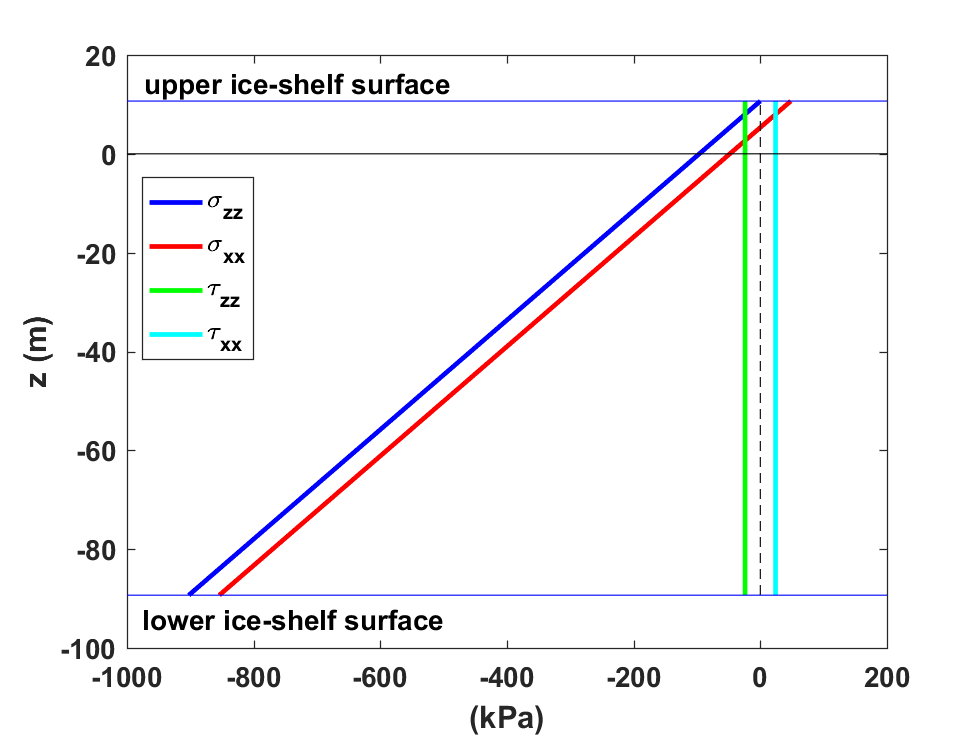
\includegraphics[width=\textwidth]{IceShelfStresses.png}
\end{subfigure}
\begin{subfigure}{0.5\textwidth}
\centering
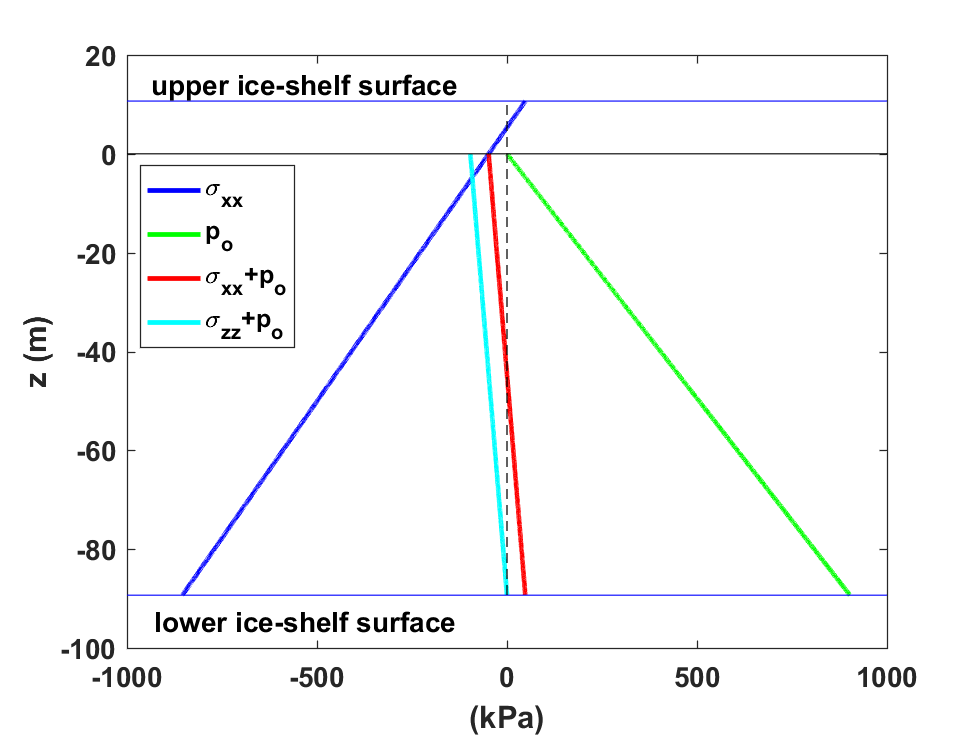
\includegraphics[width=\textwidth]{IceShelfStressesAndPressure.png}
\end{subfigure}
\caption{\label{fig:stresses}Left: Stresses within a one-dimensional
  ice shelf. Horizontal Cauchy stresses are positive at the surface
  and negative below $z=d/2$ where $d$ is the is ice shelf
  draft. Horizontal and vertical deviatoric stresses are independent
  of depth, and horizontal deviatoric stresses positive while veritcal
  deviatoric stresses are negative. Parameters:
  $\rho=910 \, \mathrm{kg\, m^{-3}}$,
  $\rho_o=1030 \, \mathrm{kg \, m^{-3}}$, $h= 100 \, \mathrm{m}$.}
\end{figure}


From (\ref{eq:sxz2}) we see that $\sxz/\tzz$ is $O(\de)$ as
expected. In contrast to the other stress terms listed above, the
shear stress $\txz$ is a first-order quantity.

Summarising, the stress tensor in an ice shelf where all transverse gradients are zero
($\partial/\partial y=0$) and $S=0$, is given by
\begin{equation}
 \bm{\sigma}= -\rho g \left ( \begin{array}{ccc} 
s/2-z & 0  & -\frac{1}{2} z \partial_x s \\
 0  & 3 s/4-z &  0 \\
 -\frac{1}{2} z \partial_x s & 0 & s-z \\ 
 \end{array} \right ),
\label{eq:shelfstresses}
 \end{equation}
and the pressure by
\[ p=\rho g (3 s/4 -z) ,
\]
and deviatoric stress tensor
\[
\bm{\tau}=\bm{\sigma}+ \bm{1} p,
\]
is 
\begin{equation}
 \bm{\tau}= \rho g \left ( \begin{array}{ccc} 
    s/4 & 0  & \frac{1}{2} z \partial_x s \\
 0  & 0 &  0 \\
 \frac{1}{2} z \partial_x s & 0 & -s/4 \\ 
 \end{array} \right ).
\label{eq:shelfdevstresses}
 \end{equation}



 Note that the sign of the horizontal stress components ($\sigma_{xx}$
 and $\sigma_{yy}$) changes with depth. At the surface ($z=s$)
 horizontal stresses are positive, at the base ($z=b$) they are
 negative. The longitudinal horizontal stresses ($\sigma_{xx}$) are
 only positive (compression) for $z>s/2$ (see
 Fig.~\ref{fig:stresses}).

The stresses in the shelf given by Eq.~(\ref{eq:shelfstresses}) are valid everywhere within the ice
shelf, in particular the stresses in the ice shelf at the grounding line are also given by
Eq.~(\ref{eq:shelfstresses}). As is evident from Eq.~(\ref{eq:shelfstresses}) the stresses,
and therefore also the strain rates, are at each location functions of local surface slope and local
ice thickness only.

Note that it has here been assumed that $S=0$, in which case $s=f$, so
one could replace $s$ with the freeboard ($f$) in the above
expressions for the stresses.


The ocean pressure, $p_o$ is
\[
 p_o=  \rho_o (S-z)
\]
for $z<S$, and therfore
\[
 \sigma_{xx}+p_o= \rho g (s/2-z) + \rho_o z
\]
for $S=0$. For $z=-\frac{1}{2} \frac{\rho}{\rho_o} h$ the sum of
horizontal stresses and ocean pressure is zero
(Fig.~\ref{fig:stresses}).

% Things to do: Side drag, solution for a floating ice shelf


% \section{Ice stream-ice shelf model}
% 
% summarizing all equations
% 
% \subsubsection{Groundin line migration}
% 
% \[
% \rho h= \rho_o b 
% \]
% where $b$ is the position of the lower ice surface. We denote the bedrock by $B(x)$. Where the ice
% is grounded, i.e.\ for $x<x_{gl}$ we have $b(x)=B(x)$, otherwise $b>B$.
% 
% 
% We write 
% \[h=h(x_{gl}(t),t) \quad \hbox{and} \quad b=b(x_gl(t),t) \]
% Differentiating with respect to $t$ gives
% \[\rho (\p_t h + \p_{x_{gl}} h \, \p_t x_{gl} ) = -\rho_o (\p_t b + \p_{x_{gl}} b \, \p_t x_{gl} ) 
% \]
% or
% \[
% \p_t x_{gl} = -\frac{rho_w \p_t b + \rho \p_t h}{\rho_o \p_x b + \rho \p_x h}
% \]
% where we have droped the subscript $gl$ from the $x$ derivative, and it is to be understood that all
% spatial derivatives are to be taken at the current position of the grounding line. Using the
% continuity equation $\p_t h+ \p_x q=a$ the above equation can also be written as
% \[
% \p_t x_{gl} = -\frac{rho_w \p_t b + \rho (a-\p_x q}{\rho_o \p_x b + \rho \p_x h}
% \]
% 
% 

\section{Steady-state geometry of a 1HD plane-strain ice sheet}

We will now derive an analytical expressions for steady-state geometry
and the velocity of a 1HD plane-strain ice sheet. The surface
mass-balance is assumed to be constant. This surface mass balance
($a$) can be thought of as the sum of the mass fluxes along the upper
($a_s$) and the lower surface ($a_b$), i.e.\ $a=a_s+a_b$.

\begin{figure}
\begin{subfigure}{0.5\textwidth}
\centering
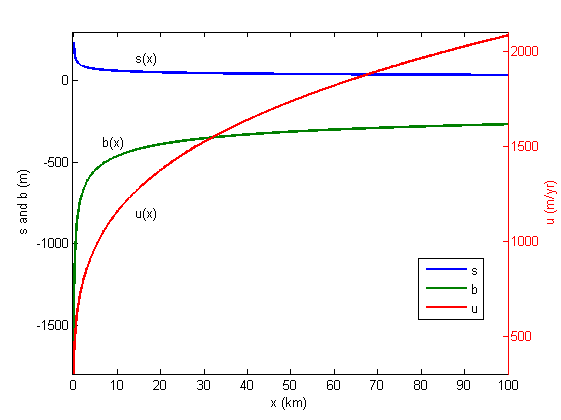
\includegraphics[width=\textwidth]{IceShelfProfile.png}
\end{subfigure}
\begin{subfigure}{0.5\textwidth}
\centering
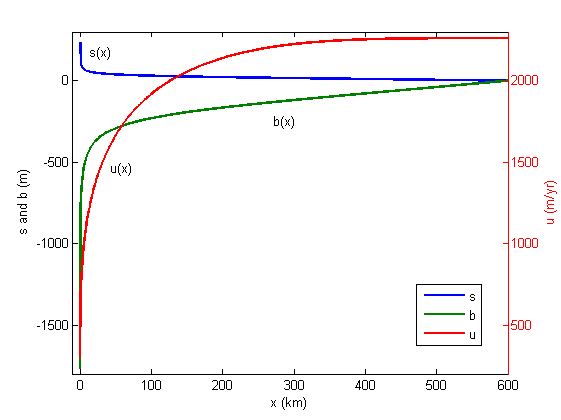
\includegraphics[width=\textwidth]{IceShelfProfileFiniteLength.png}
\end{subfigure}
\caption{\label{fig:alp}Analytical ice shelf profile.  The left hand figure is for an
  accumulation of $a=0.3\,\mathrm{m\,a^{-1}}$, while the figure on the
  right was made for $a=-1\,\mathrm{m\,a^{-1}}$. All other parameters
  are the same in both cases. Parameters: $A=1.14 \times
  10^{-9}\,\mathrm{kPa^{-3} a^{-1}}$, $n=3$, $h_{gl}=2000\,\mathrm{m}$,
  $u_{gl}=300\,\mathrm{m\,a^{-1}}$, $\rho=910 \, \mathrm{kg \,
    m^{-3}}$, $\rho_o=1030 \, \mathrm{kg \, m^{-3}}$. The value for
  $A$ corresponds to an ice temperature of about -10 degrees Celsius.}
\end{figure}

From Eq.~(\ref{eq:exx1HD}) we have
\begin{equation}
\p_x u= A \, (\varrho g h/4)^n .
\label{eq:exx1HDb}
\end{equation}
In a steady state, mass continuity requires
\begin{equation}
\p_x (uh)=a ,
\label{eq:pq}
\end{equation}
where we have used that the ice flux $q$ is $q=uh$.
Assuming constant accumulation rate we can integrate Eq.~(\ref{eq:pq}) giving
\begin{equation}
u(x) h(x) -q_{gl} = a (x-x_{gl})
\label{eq:uhq}
\end{equation}
where $x_{gl}$ is the grounding line position, and $q_{gl}=q(x_{gl})$
is the flux at the grounding line. We define the origin of the $x$
coordinates so that $x_{gl}=0$.


We also have from Eq.~(\ref{eq:pq}) \
\begin{equation}
h\, \p_x u + u \p_x h=a
\label{eq:uuh}
\end{equation}
Replacing $u$ in (\ref{eq:uuh}) using (\ref{eq:uhq}) and inserting (\ref{eq:exx1HDb})
for $\p_x u$, gives
\begin{equation}
 A h\, (\varrho g h/4)^n   +  ((a x+q_{gl})/h) \p_x h=a,
\end{equation}
which we write as
\begin{equation}
  \gamma h^{n+2}   +   (a x+q_{gl}) d_x h= a h,
\label{eq:gxh}
\end{equation}
with
\[
\gamma=A (\varrho g/4)^n \; .
\]
Separating variables
\begin{equation}
  \frac{dh}{a h-\gamma h^{n+2}} = \frac{dx}{a x+q_{gl}},
  \label{eq:gxh3}
\end{equation}
integrating both sides and simplifying gives
\begin{equation}
  h=\left ( \frac{1}{a}\left (\gamma+\frac{K}{(q+a x)^{n+1}} \right ) \right )^{-1/(n+1)},
\end{equation}
where $K$ is an integration constant.


\begin{figure}
\centering
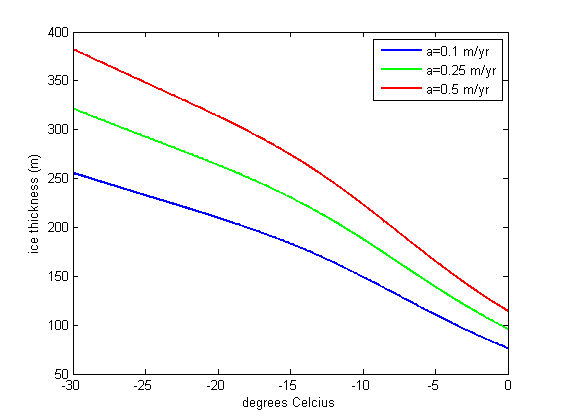
\includegraphics[width=0.75\textwidth]{1dSteadyStateIceShelf.png}
\caption{\label{fig:ssiceshelf}
Steady-state ice shelf thickness as a function of englacial
  temperature and surface accumulation.  
Parameters: $n=3$, $\rho=910 \, \mathrm{kg \,
    m^{-3}}$, $\rho_o=1030 \, \mathrm{kg \, m^{-3}}$.}
\end{figure}

We determine $K$ by specifying the
thickness at the grounding line, i.e.\
\[
h(x_{gl}=0)=h_{gl},
\]
and using $q_{gl}=h_{gl} u_{gl}$ which gives 
\[
K=q_{gl}^{n + 1}(a/h_{gl}^{n + 1}-\gamma).
\]
The solution is shown in Fig.~\ref{fig:alp}. Possibly the most
striking aspect of the solution is how quickly the thickness decreases
downstream from the grounding line.

Now that the ice geometry has been determined, the ice velocity can be
calculated directly from
\[
u=(a x+ q_{gl})/h.
\]


For $a>0$, the ice sheet is infinitely long and approaches
asymptotically the thickness $h(x\to +
\infty)=(a/\gamma)^{1/(n+1)}$. For $a<0$, the ice shelf has a finite
length $l$ given by $l=-q_{gl}/a$.

The special case $a=0$ is not covered by the above equations. One
finds that for $a=0$ the thickness distribution is given by
\begin{equation}
h=(h_{gl}^{-(n+1)}+\gamma (n+1) x/q_{gl})^{-1/(n+1)}.
\end{equation}
The above solution describes an ice shelf, with a given ice thickness
$h=h_{gl}$ at the grounding line, that spreads out in 1HD without any
addition or removal of mass. In the limit $x
\to +\infty$ the ice thickness is zero.



Note that in the above analysis we fixed the flux at the grounding
line to $q_{gl}$. We then determined the ice geometry and velocities
down-stream of the grounding line. We are here not in a position to
calculate the flux at the grounding line for a given ice thickness (or
as a function of any other aspects of the ice geometry that might
affect the flux). For a given ice thickness $h=h_{gl}$, and a given
ocean bathymetry ($B(x)$), we can however always determine possible
positions of the grounding line from the floating condition $\rho h =
\rho_o H$, where $H=S-B$ with $S$ the ocean surface and $B$ the ocean
bed.



Also note that there are two further possible solutions to the
differential equation (\ref{eq:gxh}). There is the (trivial) solution
$h=0$ and also the somewhat more interesting solution
$h=(a/\gamma)^{1/(n+1)}$.  For $a<0$ this solution can be discarded
(negative thickness). However, if $a>0$ this solution represents an
ice shelf with a constant ice thickness that is regenerated through
snow fall at the same rate that it spreads out. The ice thickness of
such a steady-state ice shelf is shown in Fig.~\ref{fig:ssiceshelf} as
a function of temperature and surface mass balance.

Another interesting fact is that the ice shelf thickness can {\em increase}
with distance downstream from the grounding line. This happens whenever
\[
h_{gl} < (a/\gamma)^{1/(n+1)} .
\]
This can be seen from an inspection of the solution shown above, or by writing
\[
u h= a x + q_{gl} ,
\]
differentiating and inserting Eq.~(\ref{eq:exx1HD}), giving
\[
u \p_x h + h A (\varrho g h/4)^n  = a ,
\]
and then using $u=(a x+ q_{gl})/h$ and solving for $\p_x h$ to arrive at
\[
\p_x h = \frac{a - \gamma h^{n+1}}{(a x + q_{gl})/h},
\]
showing that $\p_x h$ is positive for $h < (a/\gamma)^{1/(n+1)}$ .


\section{Side-drag dominated ice shelf}

We are here interested in the limiting case when all the driving
stress is balanced by side drag alone, i.e. the term $\p_x ( h \txx)$
now dropped. This is the opposite limit to the one we considered above
where $\p_x ( h \txx)$ was the dominating term and was
$\p_y (h \txy)$  was ignored.

The shallow-ice stream (SSTREAM/SSA/Shelfy) equations are
\begin{align} 
\p_x ( h ( 2 \txx + \tyy)) +\p_y ( h \txy) - \tbx
&=\rho g h \p_x s 
\label{eq:stressx}\\
\p_y (  h ( 2 \tyy + \txx)) +\p_x ( h \txy ) - \tby
&= \rho g h \p_y s 
\label{eq:stressy}
\end{align}
Over the floating section $\tbx=\tby=0$.  We assume
\begin{align*}
\eyy   &=\tyy=0 \\
\p_y \txx&=0 \\
\p_y s &= \p_y h =0 \\
\end{align*}
and ignore longitudinal streaching in the momemntum balance,
hence Eqs.~(\ref{eq:stressx}) and (\ref{eq:stressy}) become
\begin{align} 
\p_y  \txy  &= \rho g \p_x h \label{eq:stressx2}\\
\p_x ( h \txy )  &= 0  \label{eq:stressy2}
\end{align}

We integrate (\ref{eq:stressx2}) from the centerline $y=0$ to the
left-hand margin $y=w$, where the total width of the ice shelf is $2w$, i.e.

\[
\tau_m = -\varrho g w \p_x h
\]
where we $\tau_m$ is a (positive) shear stress at the margin,
i.e. $\tau_m=-\txy(y=w)$, and we have used that $\txy(y=0)=0$. We
consider the plastic case when $\tau_m$ is a yield stress and
independent of ice velocity. This simplification allows us to
calculate the ice thickness directly as
\[
h= h_c- \frac{\tau_m}{\varrho g w} (x-x_c)
\]
where $h_c$ is the ice thickenss at the calving fron
$x=x_c$. 

Eq.~(\ref{eq:stressy2}) remains correct if evaluated along the centre
line where $\txy=0$. However, it is unclear if and how this equation
can be consistent with the assumption of constant side shear stress
and variable ice thickness.


Similar to the case where a plastic formulation for basal sliding is
used, the geometry is determined directly from the yield
stress.\footnote{For a plastic symmetrical ice sheet on a flat bed
  \[ \rho g h \p_x h = \tau_b \] where $\tau_b$ is here the basal yield
  stress and therefore  $ \p_x h^2 = \frac{2\tau_b}{\rho g}$ and hence 
  \[ h^2= \frac{2\tau_b}{\rho g} |x -x_c| \] } The steady-state
velocity can then be calculated from the ice thickness distribution
using
\[
  h \p_x u + u \p_x h =0
\]
giving
\[
( \lambda -  (x-x_c) ) \; \p_x u -   u =0
\]
where
\[
\lambda=\frac{ \varrho g w h_c}{\tau_m} 
\]








\chapter{Simple 1d solution for an icestream}

\section{Problem definition:} 
Uniform ice thickness $h$ on a constant sloping bed with slope
$\alpha$. The calving front position is at $x=l$. The calving front
can be either grounded or floating, and $d$ $0\le d < \rho h /\rho_o$.


\[
4 \p_x ( h \eta \p_x u) - \beta^2 \, u= \rho g h \p_x s
\]
with
\begin{align*}
\eta&=\frac{1}{2} A^{-1/n} \, | \p_x u | ^{(1-n)/n}  \\
\beta^2&=C^{-1/m} |u|^{(1-m)/m}
\end{align*}

Boundary conditions: 
\begin{align}
u&=C \rho g h \alpha  \quad \text{at} \quad x=0 \label{eq:bc1} \\
 \tau_{xx}&=\frac{1}{4h} g ( \rho h^2 - \rho_o d^2) \quad \text{at} \quad x=l \label{eq:bc2}
\end{align}

Boundary condition \eqref{eq:bc2} can also be written as
\[
\p_x u |_{x=l} = A \left ( \frac{g (\rho h^2- \rho_o d^2)}{4 h} \right )^n
\]


\section{Solution:}
The non-linear case is
\[
\frac{2 h A^{-1/n}}{n} (\p_x u)^{1/n-1} \, \p^2_{xx} u- C^{-1/m} u^{1/m}  = - \rho g h \alpha
\]
which I'm not sure if can be solved.

However the linear case
\[
\p^2_{xx} u - \kappa^2 u  = - \frac{A \tau}{2 h} ,
\]
has the general solution
\[
u=c_1 e^{\kappa x} + c_2 e^{-\kappa x} + C \tau ,
\]
with
\[
\kappa^2=\frac{A}{2hC} ,
\]
and
\[ \tau=\rho g h \alpha \]
BCs \eqref{eq:bc1} and \eqref{eq:bc2} give
\begin{align*}
c_1 + c_2 + C \, \tau&= C \, \tau \\
c_1 \kappa e^{\kappa l} - c_2 \kappa e^{-\kappa l} &= K
\end{align*}
where
\[
K=A \frac{ g (\rho h^2- \rho_o d^2)}{4 h} .
\]
Hence
\[
u=C \tau +\frac{K \sinh \kappa x}{\kappa \cosh \kappa l}.
\]




\chapter{Grounding-line dynamics}


\begin{figure}
\centerline{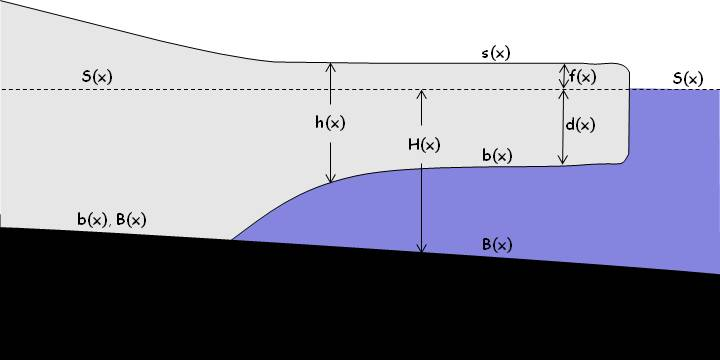
\includegraphics[width=12cm]{ProblemGeometry.jpg}}
\caption{Geometrical variables: Glacier surface ($s$)), glacier bed ($b$), ocean surface ($S$), ocean floor ($B$), 
glacier thickness ($h=s-b$)), ocean depth ($H=S-B$), glacier draft ($d=S-b$), glacier freeboard ($f=s-S$). 
\label{fig:PG2}}
\end{figure}


Here some basic aspects of grounding-line dynamics are
summarized. This is all well-known stuff from the literature.

\section{Ice-Shelf Buttressing}

Ice-shelf buttressing is defined by the impact of the ice shelf on the
stress at the grounding line. If the vertically integrated horizontal
stress state is unaffected by the ice shelf --- i.e.\ if removing the
ice shelf does not affect the state of stress at the grounding line
--- the ice-shelf provides no mechanical support to the grounding line
beside that of the ocean, and there is no ice-shelf buttressing. 



It is sometimes convenient to define a {\em buttressing parameter} $\theta$  as
\[
\theta=\frac{N}{\frac{1}{2} \varrho g h}
\]
where
\begin{equation}
N=\normalh^T \cdot ( \bm{R} \normalh)
\end{equation}
and
\[
\varrho=\rho (1-\rho/\rho_o) ,
\]
and where $\normalh$ is a normal vector pointing horizontally outwards
from the grounding line. Buttressing is the difference between the
normal stress at the grounding line with and without an
iceshelf.

In the particular case of a floating ice shelf, the field equations Eq.~(\ref{eq:FEao}) can be written as
\[
\nabla_{xy}^T \cdot (h \, \bm{R}) = \frac{1}{2} \nabla_{xy}^T ( \varrho g \rho h^2 ),
\]
Using the divergence theorem we find 
\begin{equation}
\oint \! ( \bm{R}  \cdot  \normalh - \frac{1}{2}  \varrho g \rho h  \, \normalh) \, d \Gamma  = 0 
\label{eq:Butt}
\end{equation}
The integrand is identical to the (point wise) expression of the force
balance (\ref{eq:BCCF}) at the calving front of a freely floating ice
shelf. We can split this path integral into a 1) section along the
grounding line, 2) section along the margins, and 3) section along the
calving front. If the margins do not contribute, the contribution
along the grounding line is equal to that of the calving front. Hence,
unbuttressed uniformly-wide ice shelves are passive and don't provide any buttressing. 

From Eq.~(\ref{eq:Butt}) if follows that $\theta=1$ implies no
ice-shelf buttressing. This can be taken a bit further by defining
normal and tangential buttressing numbers, but the principle is the
same: If the ice-shelf does not affect the state of stress along the
grounding line, the ice-shelf provides no buttressing.

%\[
%q \propto \theta^{n/(1/m+1)} \, h^{(n+1/m+3)/(1/m+1)}
%\]

\section{Kinematic expression for GL migration }

At the grounding line we have
\[
\rho h =\rho_o H.
\]
or simply
\[
 h=h_f
\]
At any given time $t$, this condition must always be fulfilled at the
grounding line.  Note that $H=S-B$ is independent of time, whereas
$h=s-b$ is a function of time and space, i.e.
\begin{align*}
 h&=h(x,t) \\
 H&=H(x)
\end{align*} 


We consider the rate-of-change as the grounding line
is followed, i.e.\
\begin{equation}
\left . \frac{d h_{gl}}{dt} \right |_{x=\xgl} = \frac{\rho_o}{\rho} \left . \frac{d H_{gl}}{dt}\right |_{x=\xgl}  \; ,
\label{eq:dgl}
\end{equation}
where
\[
h_{gl}=h_{gl}(t,\xgl(t))\;,
\] 
and
\[
H_{gl}=H_{gl}(\xgl(t))\;,
\] 
and therefore
\begin{equation}
\frac{d h_{gl}}{dt}=\frac{\p h_{gl}}{\p t} + \frac{\p h_{gl}}{\p \xgl} \frac{\p \xgl}{\p t}\;,
\label{eq:dhdt}
\end{equation}
and
\begin{equation}
\frac{d H_{gl}}{dt}=\frac{\p H}{\p \xgl} \frac{\p \xgl}{\p t}\;.
\label{eq:dHdt}
\end{equation}
Inserting (\ref{eq:dhdt}) and (\ref{eq:dHdt}) into (\ref{eq:dgl}) gives
\[
\p_t h + \dot{x}_{gl} \, \p_x h = \frac{\rho_o}{\rho} \dot{x}_{gl} \, \p_x H 
\]
or
\begin{align}
\dot{x}_{gl} & = \frac{\p_t h}{\frac{\rho_o}{\rho}\p_x H - \p_x h}  \label{eq:glkin1}\\
            & = \frac{\p_t h }{\p_x (h_f -  h)}                 \label{eq:glkin3}
\end{align}
where we now have skipped writing the index $gl$. All derivatives in
(\ref{eq:glkin1}) are local derivatives (but it is to be understood
that all quantities must be evaluated at the current position of the
grounding line). 


Eqs.~(\ref{eq:glkin1}) and (\ref{eq:glkin3}) are kinematic relationships,
and we refer to this equation (\ref{eq:glkin3}) as the {\em kinematic
  grounding-line equation}. It contains no additional physics beside
that of the floating condition.


At the grounding line $h_f-h=0$, and with increasing distance directly
downstream of the grounding line $h_f-h$ must increase, and hence
$\p_x (h_f -h) \ge 0$.  Therefore the grounding line must advance
whenever $\p_t h > 0$ .


One issue with using (\ref{eq:glkin1}) is that the gradient in
thickness $h$ is typically discontinuous across the grounding
line.


\section{Geometrical grounding-line migration}



Changing the sea level ($S$) causes a shift in the position of the
grounding line. This shift is only related to geometrical factors such
as ice thickness ($h=s-b$) and ocean depth bedrock ($H=S-B$). To
distinguish this shift in grounding-line position from ice-dynamical
effects, we refer to this shift as at `geometrical grounding-line
migration'. This horizontal shift in grounding line position due to
time dependent changes in the height of the ocean surface can be determined as
follows.


Ocean height ($S$) changes with time as
\[
S(t)=\bar{S}+\Delta S(t) ,
\]
but not spatially ( i.e.\ $\p_x S(t) = \p_x \bar{S} = \p_x \Delta S=0$) 

For $S=\bar{S}$ the grounding line is at  $x=\xgl$ and
\begin{equation}
\rho \, \left (s(\xgl)-b(\xgl) \right )=\rho_o (\bar{S}-B(\xgl)) .
\label{eq:mean}
\end{equation}

% Locally around the grounding line we assume a linear spatial variation
% in the geometrical variables ($s$, $b$, $B$), but we do not assume the
% up and downstream gradients to be equal. Downstream of the grounding
% line the floating condition \[ \rho (s-b)=\rho_o (S-b) \quad \hbox{for} \quad x \ge \xgl,\]
% dictates that surface and thickness slopes are related through
% \begin{align*}
% \p_x h & = -\rho_o \p_x b /\rho ,\\
% \p_x s & = - (\rho_o/\rho -1) \, \p_x b ,\\
% \p_x s & = (1-\rho/\rho_o) \, \p_x h .
% \end{align*}


For a given perturbation, $\Delta S$, in ocean height, the grounding
line moves by some distance $\Delta L$ in either up or down-stream direction. At this new grounding line
position the floating condition must again hold, and we have
\[
\rho \left (s(\xgl+\Delta L )-b(\xgl+ \Delta L ) \right )=\rho_o (\bar{S}+\Delta S-B(\xgl+\Delta L)) 
\]
or
\[
\rho (s(\xgl) + \p_x s \Delta L -b(\xgl) - \p_x b  \Delta L )=\rho_o (\bar{S}+\Delta S-B(\xgl) - \p_x B \Delta L)) 
\]
(For notational simplicity we have not indicated in the above equation
that the derivatives are to be evaluated on both sides of the
grounding line and that they are in fact directional derivatives in
the up and down-stream directions.)  Using (\ref{eq:mean}) gives
\[
\rho (\p_x s - \p_x b  ) \Delta L=\rho_o (\Delta S- \p_x B \Delta L)) 
\]
or
\begin{equation}
\Delta L^{+/-} = \frac{\rho_o \Delta S}{\rho (\p_x s^{+/-} - \p_x b^{+/-} ) + \rho_o \p_x B^{+/-}}
\label{eq:dLtide}
\end{equation}
Eq.~(\ref{eq:dLtide}) is valid even if the derivatives are not
constant across the location of grounding line ($\xgl$) at mean tide
($\Delta S=0$). We have indicated this by adding the superscript
$+/-$. Here $\Delta S$ is positive for a high tide, and negative for a
low tide. At low tide the gradients downstream of $\xgl$ are to be
used (minus sign), and at high tide the gradients upstream of $\xgl$
(positive sign).


\begin{figure}
\centerline{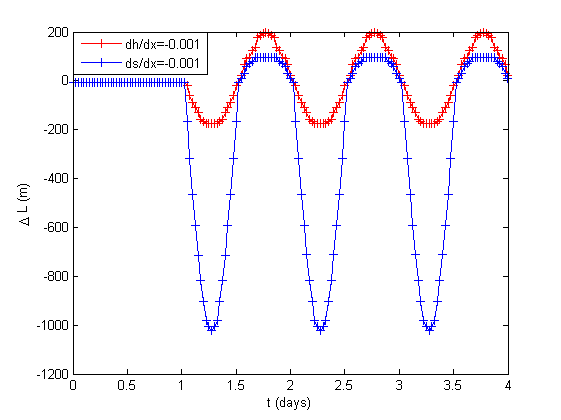
\includegraphics[width=8cm]{dLTide.png}}
\caption{Example of grounding line migration in response to tidal
  forcing using the hydrostatic assumption. The curves were calculated
  using the flow model \'Ua which is a vertically integrated flow
  model that calculates grounding line positions using the hydrostatic
  assumption. The red curve was calculated for a constant surface
  slope of $ds/dx=-0.001$ and blue curve for a constant thickness
  gradient of $dh/dx=-0.001$. In both cases the bedrock gradient as
  $dB/dx=-0.01$. The tidal amplitude was 2 m and the tidal period 1 d.
  To suppress the effects of ice flow the flow parameters were set to
  values that made the ice effectively rigid and basal sliding was
  enforced to be close to zero. 
\label{fig:dLTide}}
\end{figure}


If $\p_x B$ is the same on both sides of the $\xgl$, then it follows
from (\ref{eq:dLtide}) that the shifts in grounding line position at
high and low tides are only equal in magnitude provided $\p_x h$ is
the same on both sides of $x=\xgl$ as well. In other words, for a
constant bed slope, a tidally-induced grounding line migration is
symmetrical if, and only if, the thickness gradient does not change
across the grounding line. Conversely, if the thickness
gradients are not equal on both sides of the grounding line, the
grounding line movement will always be asymmetric with respect to the tidal
cycle.

Such an asymmetrical grounding line migration takes place if,
for example, the upper surface gradient ($\p_x s$) is constant across
the grounding line. In that case the thickenss gradient cannot be
equal on both sides of $x=\xgl$ as well.  There is then a break in
thickness gradient at $x=\xgl$ given by
\[
\p_x h= \begin{cases} \p_x h^{+}=\p_x s - \p_x B & \text{for } x \leq \xgl \\
                      \p_x h^{-}=\p_x s/(1-\rho/\rho_o) & \text{for } x \geq \xgl
        \end{cases} 
\]
(There is no need to use the superscripts $+/-$ with $\p_x s$ and
$\p_x B$ in the above equation because here we are assuming that those
derivatives are continous across the grounding line.)  When this
expresson for the break in thickness gradient is inserted in
(\ref{eq:dLtide}) we find that the migration distance $\Delta L^{-}$
at a low tide (when $S=\bar{S}-\Delta L$), is given by
\[
\Delta L^{-} = - \frac{\Delta S}{\frac{\rho/\rho_o}{1-\rho/\rho_o} \p_x s + \p_x B} ,
\]
and at a high tide by
\[
\Delta L^{+} = \frac{\Delta S/(1-\rho/\rho_o) }{\frac{\rho/\rho_o}{1-\rho/\rho_o} \p_x s + \p_x B} ,
\]
and that
\[
|\Delta L^{-}| = (1-\rho/\rho_o) | \Delta L^{+}| .
\] 
In the case of a constant surface gradient, the upstream
grounding-line shift at high tide is therefore about 9 times as large
as the downstream shift at low tide.



In general we expect neither the thickness nor the surface gradient to
be constant across the grounding line. Since the migration is only
symmetrical in the particular case of a constant thickness gradient
across the grounding line, we expect an asymmetrical grounding line
migration in response to tides to be the general rule rather than an exception.



An example of transient hydrostatic grounding-line migration in
response to tides is shown in Fig.~\ref{fig:dLTide}. The migration was
calculated using the flow model \'Ua. This model, as do most commonly
used flow model in glaciology, assumes that the grounding line is
always exactly where the hydrostatic floating condition $\rho h=\rho_o
(S-b)$ is met. The modelled grounding line displacements are in a good
agreement with those calculated using Eq.~(\ref{eq:dLtide}). For
example, in the case of constant surface slope the modelled values are
$\Delta L^{-}=105$ m and $\Delta L^{+}=-1013$ while those based on
Eq.~(\ref{eq:dLtide}) are $\Delta L^{-}=109$ m and $\Delta
L^{+}=-1020$. These differences of a few meters are considerably
smaller than the spatial dimension of 85 m of the smallest element of
the mesh used in this particular run by the FE-model \'Ua.





\section{Flux at the grounding line}
\label{sec:FGL}
%\setcounter{equation}{0}

Upstream from the grounding line
\begin{equation}
  2 \p_x \left (h A^{-1/n} \, | \p_x u|^{1/n-1} \; \p_x u \right ) - C^{-1/m} |u|^{1/m-1} \; u = \rho g h \, \p_x s
\label{eq:fu}
\end{equation}
In terms of stresses this equation can also be written as
\begin{equation}
  2 \p_x (h \txx) -t_{bx}= \rho g h \p_x s
\label{eq:fs}
\end{equation}


Boundary conditions at the grounding line where $x=\xgl$ are
\begin{align}
\p_x u &= A (\varrho g h/4)^n  \label{eq:We3} \\
     h&=\rho_o H /\rho . \label{eq:fc}
\end{align}
Note that boundary condition (\ref{eq:We3}) can be rearanged as
\[
2 A^{-1/n} (\p_x u)^n = \frac{1}{2} \varrho g h
\]
If we insert the above expression into (\ref{eq:fu}), assuming $\p_x u > 0$, then we arrive at
\[
\frac{1}{2}\varrho g \p_x h^2  - t_{bx} = \rho g h \p_x s
\]
If we now assume that $\p_x s \approx \p_x h$ upstream of the
grounding line, for example by setting $s=B+h$ with $\p_x B=0$ for $x>\xgl$, we
obtain
\begin{equation}
[\frac{1}{2} \varrho g \p_x h^2] - [t_{bx}] = [\frac{1}{2} \rho g \p_x h^2]
\label{eq:ghp}
\end{equation}
where the brackets are used to indicate that we are here simply
comparing sizes of terms, and where we have writtin $ h \p_x h = \frac{1}{2} \p_x h^2 $

Since $\varrho \approx \rho/10$ is it
clear that the first term on the left-hand side of (\ref{eq:ghp}) is
small compared to the right-hand side, and that the right-hand side
must therefore be approximately balanced by the second term on the
left-hand side of (\ref{eq:ghp}), i.e.
\begin{equation}
  [t_{bx}] = [-\frac{1}{2} \rho g \p_x h^2].
\label{eq:ghp2}
\end{equation}
Note that the key assumption here is that
$\p_x s \approx \p_x h$ for $x < \xgl$.

Downstream of the
grounding line, flotation implies that $\p_x s = \varrho \p_x h/\rho$
(see Eq.~\ref{eq:hs1}) and if, for example, $\p_x s \approx 
\varrho \p_x h / \rho$, upstream of the grounding line we instead of
(\ref{eq:ghp}) arrive at
\begin{equation}
[\frac{1}{2}\varrho g h^2] - [t_{bx}] = [\frac{1}{2} \varrho g  \p_x h^2]
\label{eq:ghp2}
\end{equation}
and clearly now it is the first term on the left-hand side that balances the right-hand
side.



We will now derive an approximation for the flux at the grounding line
as a function of (local) ice thickness, and start by making the
assumption that $\p_x s \approx \p_x h$ in which case as we have seen
\[
t_{bx} \approx - \rho g h \p_x s ,
\]
i.e.\ that the second term on the left-hand sides of (\ref{eq:fu}) and
(\ref{eq:fs}) is now approximately balanced by their respective right-hand
sides.  Hence, using Weertman sliding law we have
\begin{equation}
   u = C (-\rho g h \p_x h )^m ,
\label{eq:uch}
\end{equation}
where we have anticipated that $\p_x h$ will be strictly negative. 


In a steady state
\begin{equation}
  \p_x (uh) = a , \label{eq:ass}
\end{equation}
which allows us to write
\begin{equation}
 \p_x h =(a- h \p_x u)/u .
\label{eq:ahu}
\end{equation}
Inserting the boundary condition (\ref{eq:We3}) into (\ref{eq:ahu}) gives
\begin{equation}
\p_x h =(a- h A (\varrho g h/4)^n )/u ,
\label{eq:ahA}
\end{equation}
and then inserting (\ref{eq:ahA}) into (\ref{eq:uch}) and assuming that $a \ll
h A (\varrho g h/4)^n $ gives
\begin{equation}
   u = C \left (\rho g h h A \left (\rho g \delta g h/4 \right )^n /u \right )^m .
\label{eq:uch2}
\end{equation}

or
\[
u^{m+1}=  4^{-n m}\, C \,  A^m (g \rho)^{m+n m} \delta^{n m}  \;  h^{n m + 2 m} ,
\]
where $\delta$ is defined as
\[
\delta := 1- \rho/\rho_o
\]
The ice flux  $q=uh$ at the grounding line is therefore
\begin{equation}
q=  \left [ 4^{-n m} \, C \, A^m  (g \rho)^{m+n m} \; \left (1-\rho/\rho_o \right )^{n m}  \right ]^{1/(m+1)}  \; h^{(n m + 3 m + 1)/(m+1)} ,
\label{eq:Schoofhq}
\end{equation}
where\footnote{For $q=\rho u h$ and keeping the $\theta$ term we have
\[
q=\rho  \left ( 4^{-n} C^{1/m} A (\rho g)^{n+1} \delta^n  \right )^{m/(1+m)} \, \theta^{nm/(1+m)} \,  h^{(n m +3 m+1)/(1+m)} 
\]
} $h$ is the thickness at the grounding line, i.e.
\[
h=h_{\mathrm{gl}}=\rho_o H /\rho.
\]
The relationship between flux relationship (\ref{eq:Schoofhq}) is
identical to that of Schoof's `B' model.  We arrived at this flux
relation ship by assuming that velocity at the grounding line is given
by the SIA relationship, and that $\p_x u$ at the grounding line is
given by the boundary condition (\ref{eq:We3}) for horizontal strain
rates. In addition we assumed steady-state conditions and that $a
\ll h \p_x u$.


Note that, as Eq.~(\ref{eq:uch2}) shows, it is possible to express the
velocity at the grounding line as a function of the ice thickness $h$
alone, i.e.\ without any reference to the surface slope $\p_x h$. This
is possible because the surface slope at the grounding line is related
to thickness through Eq.~(\ref{eq:ahA}). We were able to use the
boundary condition (\ref{eq:We3}), the mass conservation equation
(\ref{eq:ass}), and the simplified momentum equation (\ref{eq:uch}) to
arrive at Eq.~(\ref{eq:uch2}), giving velocity at the grounding-line
as a function of thickness alone. 


\section{Balance between terms on both side of the grounding line}

%\setcounter{equation}{0}
(What follows is basically a slighly different framing of the argument in
section \ref{sec:FGL} used to show that the basal shear traction will
balance the driving stress upstream of the grounding line, provided
$\p_x s \approx \p_x h$.)

Field equation and boundary condition at the
grounding line written in terms of velocity are
\begin{align}
2 A^{-1/n} \p_x \left (h |\p_x u|^{(1-n)/n} \, \p_x u \right ) - \He(h-h_f) \, C^{-1/m} \, |u|^{(1-m)/m} u & = \rho g h \p_x s  \label{eq:velssa}\\
2 A^{-1/n} h |\p_x u|^{(1-n)/n}   \, \p_x u  = \frac{1}{2} \varrho g \, h^2   \quad & \text{at} \quad x=\xgl\label{eq:bc1b} \\
h=h_f     \quad & \text{at} \quad x=\xgl\label{eq:bc2b}
\end{align}

where $\He$ is the Heaviside step function, and
where
\[
h_f=\rho_o H/\rho
\]
and where $\varrho=\rho (1-\rho/\rho_o)$. 

Inserting (\ref{eq:bc1b}) into (\ref{eq:velssa}) and assuming that over the grounded area 
$ |\p_x s| \gg |\p_x b|$, and therefore that $\p_x h = \p_x s - \p_x b \approx \p_x s $, we arrive at
\[
\frac{1}{2} \varrho g \p_x \left ( h^2  \right ) - \He(h-h_f) \, C^{-1/m} \, |u|^{(1-m)/m} u = \rho g h \p_x h  \label{eq:velssa2}
\]
or
\[
\frac{1}{2} \varrho g \p_x  h^2  - \He(h-h_f) \, C^{-1/m} \, |u|^{(1-m)/m} u = \frac{1}{2} \rho g  \p_x h^2  \label{eq:velssa3}
\]
which immediately shows that the first term on the left hand side is
$\varrho /\rho=\rho (1-\rho/\rho_o))/\rho=(1-\rho/\rho_o) \approx 0.1 $
the size of the right-hand side.

Downstream of the grounding line $s=(1-\rho_o/\rho) h$ and therefore
$\p_x s = \delta \p_x b \approx 0.1 \p_x b$, or
$\p_x s \ll \p_x h $ and this reversal of the relative sizes of the upper
and lower slopes ensures that we now also have the right balance
downstream of the grounding line, where the first term on the left-hand side now equals the right-hand side.




\section{GL scalings  (Schoof)}

\setcounter{equation}{0}
Field equations written in terms of velocity and stresses, respectively, are
\begin{align}
2 A^{-1/n} \p_x \left (h |\p_x u|^{(1-n)/n} \, \p_x u \right ) - \He(h-h_f) \, C^{-1/m} \, |u|^{(1-m)/m} u & = \rho g h \p_x s  \label{eq:vel}\\
     2 \p_x \left ( h \txx \right )  - \tau_b & = \rho g h \p_x s  \label{eq:stress} 
\end{align}
where $\He$ is the Heaviside step function.
Boundary conditions at $x=\xgl$ are
\begin{align}
2 A^{-1/n} h |\p_x u|^{(1-n)/n}   \, \p_x u & = \frac{1}{2} \varrho g \, h^2  \label{eq:bc1c} \\
h&=h_f   \label{eq:bc2c}
\end{align}
where
\[
h_f=\rho_o H/\rho
\]
and where $\varrho=\rho (1-\rho/\rho_o)$. The above model is only valid for $[z]/[x] \ll 1 $
and $u_d/u_b\ll 1$, where $u_d$ is the deformational velocity and
$u_b$ the sliding velocity.


Scalings: With $[u]$ and $[x]$ as scales for the horizontal velocity
and the span of the ice sheet, the kinematic boundary condition suggests
\[
\frac{[u] [z]}{[x]}= [a] \quad \hbox{and} \quad [t]=\frac{[x]}{[u]}
\]
We set a scale for $C$ by writing
\[
[u]^{1/m}/[C]^{1/m}=\rho g [z] [z]/[x]
\]
i.e.\ we balance basal shear stress with the driving stress.
%Is this not
%equivalent to assuming that $\tau_b \approx \tau_d$ where $\tau_d
%=\rho g h \p_x s$ and that $[s]=[z]$. As a consequence the second term
%on the right-hand sides of (\ref{eq:vel}) and (\ref{eq:stress}) is
%(for grounded ice) always of same order as the right-hand side.
We introduce
\begin{equation}
  \epsilon=\frac{\txx}{\sxx} = \frac{A^{-1/n} ([u]/[x])^{1/n}}{2 \rho g [z]} 
\end{equation}
and will consider the case $\epsilon \ll 1$, and we also define
\begin{equation}
  \delta=1-\rho/\rho_o  
\end{equation}
where $\delta\approx 0.1$.


Inserting these scalings into field equation (\ref{eq:vel}) and the boundary condition (\ref{eq:bc1c})
gives
\begin{align}
4 \epsilon \, \p_x \left (h |\p_x u|^{(1-n)/n} \, \p_x u \right ) - |u|^{(1-m)/m} u & = h \, \p_x s \quad \text{for} \quad x<\xgl \label{eq:velscaled}\\
|\p_x u|^{(1-n)/n} \, \p_x u&= \frac{\delta h}{8 \epsilon} \quad \text{at} \quad x=\xgl \label{eq:bc1scaled}
\end{align}


%\subsection{Local analysis (argument by Victor Tsai)}


Summarizing the scaled momentum equations are
\begin{align}
4 \epsilon \, \p_x \left (h |\p_x u|^{(1-n)/n} \, \p_x u \right ) - |u|^{(1-m)/m} u & = h \, \p_x s \quad \text{for} \quad x<\xgl \label{eq:velscaled2}\\
|\p_x u|^{(1-n)/n} \, \p_x u&= \frac{\delta h}{8 \epsilon} \quad \text{at} \quad x=\xgl \label{eq:bc1scaledb}
\end{align}


Now we consider the scaled momentum equation (\ref{eq:velscaled}) in the
vicinity of the grounding line. As we approach $x \to \xgl$ from
the upstream side we expect the first term on the left-hand side of
(\ref{eq:velscaled}) to be given by (\ref{eq:bc1scaled}). Inserting
(\ref{eq:bc1scaled}) into (\ref{eq:velscaled}) gives
%\begin{equation}
%4 \epsilon \, \p_x \left (h \delta h /(8 \epsilon) \right ) - |u|^{(1-m)/m} u  = h \, \p_x s ,
%\label{eq:sc2}
%\end{equation}
%or
\begin{equation}
\delta  \, h \, \p_x h   - |u|^{(1-m)/m} u  = h \, \p_x s ,
\label{eq:sc3}
\end{equation}
all quantities evaluated at the grounding line.

Now consider the right-hand side of the above equation
We always have
\[ 
\p_x s= \p_x (h+b) ,
\]
Upstream of the grounding line we do not expect $\p_x b$ to be related
(at least not in some simple way) to $\p_x h$. Consider the case
$\p_x b=0$ while $\p_x h$ takes some finite value, then
equation (\ref{eq:stress}) is
\begin{equation}
\delta \, h \p_x h  - |u|^{(1-m)/m} u  = h \, \p_x h  ,
\label{eq:sc4}
\end{equation}
and since $\delta \ll 1$ (in fact $\delta \approx 0.1$) the second
term on the left-hand side approximately balances the right-hand
side. We therefore have an approximate balance between basal stress
and driving stress.

In physical terms the situation down-stream of the grounding line is clear. There the
first term on the left-hand side must balance the term on the right
hand side. Here our formulation gives the right balance because since  $\p_x
b$ and $\p_x h$ are related by the floating condition
\[
\p_x s= \p_x(h+b)=\p_x (h-(1-\rho/\rho_o) h)=\delta \; \p_x h ,
\]
and when inserted into 
\begin{equation}
 \frac{1}{2} \delta \; \p_x \left (h h \right )  = \delta \; h \, \p_x h  ,
\label{eq:sc40}
\end{equation}
we arrive, which is the right balance.

Summarizing, if $h$ and $b$ are related
through the floating condition, the balance is always between the
first lhs term and the rhs, but  the balance is between the second rhs
term and the lhs if
\[
|\p_x b| \ll |\p_x h|
\] 
In the particular case $\p_x b=0$ the balance is always
between the basal shear stress term and the driving stress.


\section{Grounding-line instability}

For a steady state with the grounding line located at $x=\xgl$, mass
conservation requires
\[
\gamma \; \xgl + q(\xgl)=0
\]
where we have assumed that the ice divide is ast $x=0$ and the surface
mass balance is $\gamma$. We assume the surface mass balance is spatially constant and
positive, i.e.\ $\gamma > 0$. Clearly if $\gamma<0$, no ice sheet is possible. 

Perturb $\xgl$ by $\Delta x$
\[
  \xgl'=\xgl + \Delta x
\]

If
\[
\gamma \; \Delta x - \p_x q \; \Delta x < 0
\]
then more ice flows across the grounding line than is added over the
new surface $\Delta x$ upstream of the grounding line. The volume of
the (grounded) ice sheet must decrease with time and the grounding
line must retreat towards the original steady state. (Note that the
derivative of $q$ with respect to $x$ is the derivative of $q$
following the grounding-line position.)


Hence, if
\[
  \p_x q > \gamma
\]
then the grounding line is stable, but
\begin{align*}
  \frac{\p q}{\p x} &= \frac{\p q}{\p h} \frac{\p h}{\p x} \\
  &= \frac{\p q}{\p h} \frac{\rho_o}{\rho} \frac{\p (S-B)}{\p x}\\
  &= -  \frac{\rho_o}{\rho}\frac{\p q}{\p h} \frac{\p B}{\p x}
\end{align*}
For a prograde bed, $\p_x B <0$, and therefore we must have $\p_h q >0$
for the grounding line to be stable. Conversely, for a retrograde bed where $\p_x
B > 0$ we must have $\p_x q <0$ for the grounding line to be stable.

\part{Appendices}
\appendix



\chapter{Calculating vertical surface velocity}

The sign convention for upper- and lower-surface mass balance is such
that the kinematic boundary conditions at the upper and
lower surfaces read, respectively,
\begin{align} 
\p_t s + u \p_x s +v \p_y s -w_s&=a_s  ,\label{eq:pts} \\
\p_t b + u \p_x b +v \p_y b -w_b&=-a_b ,\label{eq:ptb} 
\end{align}
i.e.\ adding ice is always defined as positive surface mass balance.

Subtracting \eqref{eq:ptb} from \eqref{eq:pts} gives
\[
\p_t h+ u \, \p_x h +v \, \p_y h -w_s + w_b=a_s+a_b ,
\]
where it has been used that $u$ does not change with depth. Now using \eqref{eq:sb} gives
\[
\p_t h+ u \, \p_x h + v \, \p_y h +h ( \exx + \eyy)=a_s+a_b,
\]
or
\begin{equation}
\p_t h+ \p_x (u h) + \p_y ( v h)=a_s+a_b,
\label{eq:conc}
\end{equation}
hence, in the flux-conservation equation both upper and lower mass balance terms have the same sign. 




\section{grounded part}

On the grounded part $\p_t s =\p_t h$ and the kinematic boundary condition gives
\begin{equation}
w_s=\p_t h  + u \, \p_x s + v \, \p_y s -a_s ,
\label{eq:wsg}
\end{equation}
but this requires $\p_t h$ to be known before we can calculate $w_s$. An alternative approach is to 
integrate the vertical strain rate $\ezz$ over the thickness, use the mass conservation equation and
the fact that horizontal strain rates do not change across the thickness, to arrive at
\begin{equation} 
w_s= w_b-h \, ( \exx + \eyy) .
\label{eq:sb} \end{equation}
We now calculate $w_b$ from the kinematic boundary condition at the lower surface as
\[
w_b=a_b + u \p_x b + v \p_y b ,
\]
and insert into \eqref{eq:sb} arriving at
\begin{equation} 
w_s= a_b + u \, \p_x b + v \, \p_y b -h \, ( \exx + \eyy) ,
\label{eq:wsgrounded} 
\end{equation}
which represents a convenient way of calculation $w_s$ once the horizontal velocity field has been determined.



\section{floating part}
Where the ice is afloat 
\[
s = S+(1-\rho/\rho_o) \, h 
\]
i.e.\
\[
\p_t s =  (1-\rho/\rho_o) \, \p_t h 
\]
The kinematic boundary condition at the surface gives
\[
w_s=\p_t s + u \, \p_x s + v \, \p_y s -a_s 
\]
and therefore
\begin{equation}
w_s=(1-\rho/\rho_o) \, \p_t h  + u \, \p_x s + v \, \p_y s -a_s 
\label{eq:wsfloating}
\end{equation}
If $\p_t h$ is known \eqref{eq:wsfloating} can be used to calculate $w_s$, otherwise
we use (\ref{eq:conc}) and find that
\begin{equation}
w_s=(1-\rho/\rho_o) \, (a_s+a_b - \p_x q_x - \p_y q_y)  + u \, \p_x s + v \, \p_y s -a_s 
\label{eq:wsfloating2}
\end{equation}


An alternative way of calculating $w_s$ is to insert the floating condition
\[ 
s=(1-\rho_o/\rho) b 
\]
into (\ref{eq:pts}) and to use (\ref{eq:ptb}) to get rid of $\p_t b$ 
\begin{equation} 
(1-\rho_o/\rho) (w_b-a_b-u \p_x b-v p_y b) + (1-\rho_o/\rho) (u \p_x b + v \p_y b) -w_s =a_s 
\label{eq:pts2} 
\end{equation}
to arrive at the simple and intuitive expression
\begin{equation} 
(1-\rho_o/\rho) (w_b-a_b)  =a_s+w_s 
\label{eq:pts3} 
\end{equation}
and then to use the (\ref{eq:sb}) to get rid of $w_b$ leading to
%\[ 
%(1-\rho_o/\rho) (w_s-a_b+h(\exx+\eyy))=a_s+w_s 
%\]
%or
%\[ w_s (-\rho_o/\rho)  +    (1-\rho_o/\rho) (-a_b+h(\exx+\eyy))=a_s  \]
%\[ (1-\rho_o/\rho) (-a_b+h(\exx+\eyy))-a_s = w_s \rho_o / \rho \]
\begin{equation} 
 w_s =  -(1-\rho/\rho_o)\,  \left (h(\exx+\eyy) - a_b\right ) - a_s \, \rho /\rho_o  
\label{eq:wsfloating3}
\end{equation} 
The above expression shows that adding ice to the surface ($a_s>0$)  causes neg.\ vertical
surface velocity, as does horizontal divergent flow ($\exx+\eyy>0$), and basal melting ($a_b<0$).



\chapter{Integral theorem}

If $f$ and $g$ are scalar functions then in $x$ and $y$ directions we have
\begin{align}
\int_{\Omega} f \, \p_x g \; d \Omega &= - \int_{\Omega} \p_x f \, g \; d \Omega + \oint_{\p \Omega} f \, g \, n_x \; d \Gamma \\
\int_{\Omega} f \, \p_y g \; d \Omega &= - \int_{\Omega} \p_y f \, g \; d \Omega + \oint_{\p \Omega} f \, g \, n_y \; d \Gamma
\end{align}
If we write $g=g_x$ in the upper one and $g=g_y$ in the lower one, add
them together and define $\bm{g}=(g_x,g_y)^T$ and
$\hat{\bm{n}}=(n_x,n_y)^T$ then we arrive at
\begin{equation}
\int_{\Omega} f \, \nabla_{xy} \cdot \bm{g} \; d \Omega = -
\int_{\Omega} \nabla_{xy} f \cdot \bm{g} \; d \Omega + \oint_{\p
  \Omega} f \, \bm{g} \cdot \hat{\bm{n}} \; d \Gamma \\
\label{eq:fgg}
\end{equation}



\chapter{Definition of gradients in terms of directional derivatives and inner products}
\chaptermark{Gradients and inner products}

Sensitivities are directional derivatives. The directional derivative
of the scalar function $J(p)$ in the direction $\phi$
is denoted by $D f(p)[\phi]$ and defined as
\begin{align*}
 D f(p)[\phi] &= \lim_{\epsilon \to 0} \frac{d}{d \epsilon} f(p+\epsilon \phi)  \\
               &= \lim_{\epsilon \to 0}  \frac{f(p+\epsilon \phi)-f(p)}{\epsilon}
\end{align*}

The directional derivative is sometimes written as $\delta f(p,\phi)$
or as $f'(p,\phi)$ i.e.
\[
D f(p)[\phi]=f'(p,\phi)=\delta f(p,\phi)
\]
are just different ways of writing the directional derivative.

We define the gradient through 
\[
 D f(p)[\phi]  = < \nabla J(p), \phi >_H
\]
where $H$ is a Hilbert space and $f: H \to \mathbb{R}$. 
Here $\nabla J(p)$ is the gradient of $J$, and the expression above
{\em defines} the gradient in terms of the (directional) derivative
for a given inner product.

In other words, for a function $f:H \to \mathbb{R}$ the gradient is
defined as the Riez-representation for the directional derivative
$D f(p)[\phi]$ through
\[
< \nabla f (p) , \phi>_H= D f(p)[\phi] 
\]
The directional derivative depends on the inner product $< , >_H$ and
the gradient is not defined without specifying the inner product.

Example: Consider the case $H=\mathbb{R}^n$ with the inner product 
\[
<\bm{x},\bm{y}> = \bm{x}^T \bm{M} \bm{y}
\]
where $M$ is symmetric and positive definite (for example the mass
matrix or any covariance matrix.)

The directional derivative is
\[
D f(p)[\phi]=\frac{\p f}{\p p_q} \phi_q = < M^{-1} \p f / \p p_q, \phi_q> 
\]
and therefore 
\[
 \nabla f = [ M^{-1}]_{pq} \; \p f /\p \phi_q  
\] 

Had we instead used the Euclidean inner product as $<\bm{x},\bm{y}> = \bm{x}^T
\bm{y}$
the corresponding Euclidean gradient would be 
\[
 [\nabla_E f ]_p = \p f /\p \phi_q  
\] 
or
\[
 \nabla f  = M^{-1} \, \nabla_{E} f
\]
where the subscript $E$ denotes the Euclidean gradient. This
distinction becomes important in the application of the adjoint method
where we obtain a gradient that is dependent on the natural FE inner
product 
\begin{align*}
< f , g> &= \int f \, g \, dA \\
         &=\int f_p \, \phi_p  \, g_q \, \phi_q  dA\\
         &= \bm{f} M \bm{g} 
\end{align*}
Hence in FE the dual pairing is 
\[
< f , g > = \bm{f}^T \bm{M} \bm{g}
\]
where $f$.

The adjoint $L^\ast$ of a given operator $L$ is defined as
\[
< L^\ast f, g > =< f, L g>  
\]
for any $f$ and $g$. 

If we are working in $H_1=\mathbb{R}^{d_1}$ and the dual space is
$H_2=\mathbb{R}^{d_2}$ and
\[
 < f ,g >_{H_1 , H_2} = \bm{f}^T \bm{g}
\]
and
\[
< L^\ast f, g >_{H_1 , H_2}  =< f, L g>_{H_1 , H_2}   
\]
and we denote by $\bm{L}$ and $\bm{L}^\ast$the matrix representations
of the continuous linear operators $L$ and $L^\ast$, respectively,
then 
\[
 \bm{L}^\ast = \bm{L}^T
\]

If,  on the other hand, we have the dual pairings
\[
 < f ,g >_{H_1 , H_2}  = \bm{f}^T \bm{M} \bm{g}
\]
where $\bm{M}$ is a positive definite matrix, then
\[
\bm{L}^\ast=\bm{M}^{-T} \bm{L}^T \bm{M}^T
\] 
as can be seen as follows
\begin{align*}
 <M^\ast f, g> &= < f, L g> \\
              &= \bm{f}^T \bm{M} ( \bm{L} \bm{g}) \\
              &= \bm{f}^T \bm{M} \bm{L} \bm{M}^{-1} \bm{M}  \bm{g} \\
              &= (\bm{M}^{-T} \bm{L}^T \bm{M}^T \bm{f})^T  \bm{M}  \bm{g} \\
              &= <\bm{M}^{-T} \bm{L}^T \bm{M}^T \bm{f} ,  \bm{g}) \\
\end{align*}

We can generalise this a bit further and consider the case where the
dual space has a different dimension with
\begin{align*}
  <f,f>_{H_1 H_1} &= \bm{f}^T \bm{M}_1 \,\bm{f} \\
  <g,g>_{H_2 H_2} &= \bm{g}^T \bm{M}_2 \, \bm{g}
\end{align*}
and find that 
\[
\bm{L}^\ast=\bm{M}_1^{-T} \bm{L}^T \bm{M}_2^T
\]


\end{document}
 
